\documentclass[11pt]{aghdpl}
% \documentclass[en,11pt]{aghdpl}  % praca w języku angielskim

% Lista wszystkich języków stanowiących języki pozycji bibliograficznych użytych w pracy.
% (Zgodnie z zasadami tworzenia bibliografii każda pozycja powinna zostać utworzona zgodnie z zasadami języka, w którym dana publikacja została napisana.)
\usepackage[english,polish]{babel}

% Użyj polskiego łamania wyrazów (zamiast domyślnego angielskiego).
\usepackage{polski}

\usepackage[utf8]{inputenc}

% dodatkowe pakiety

\usepackage{mathtools}
\usepackage{amsfonts}
\usepackage{amsmath}
\usepackage{amsthm}

% --- < bibliografia > ---

% \usepackage[
% style=numeric,
% sorting=none,
% %
% % Zastosuj styl wpisu bibliograficznego właściwy językowi publikacji.
% language=autobib,
% autolang=other,
% % Zapisuj datę dostępu do strony WWW w formacie RRRR-MM-DD.
% urldate=iso8601,
% % Nie dodawaj numerów stron, na których występuje cytowanie.
% backref=false,
% % Podawaj ISBN.
% isbn=true,
% % Nie podawaj URL-i, o ile nie jest to konieczne.
% url=false,
% %
% % Ustawienia związane z polskimi normami dla bibliografii.
% maxbibnames=3,
% % Jeżeli używamy BibTeXa:
% backend=bibtex
% ]{biblatex}
\usepackage[backend=biber,style=numeric,sortcites,natbib=true,sorting=none]{biblatex}

\usepackage{csquotes}
% Ponieważ `csquotes` nie posiada polskiego stylu, można skorzystać z mocno zbliżonego stylu chorwackiego.
\DeclareQuoteAlias{croatian}{polish}

\addbibresource{biblio.bib}

% Nie wyświetlaj wybranych pól.
%\AtEveryBibitem{\clearfield{note}}


% ------------------------
% --- < listingi > ---

% Użyj czcionki kroju Courier.
\usepackage{courier}

\usepackage{listings}
\lstloadlanguages{TeX}

\lstset{
	literate={ą}{{\k{a}}}1
           {ć}{{\'c}}1
           {ę}{{\k{e}}}1
           {ó}{{\'o}}1
           {ń}{{\'n}}1
           {ł}{{\l{}}}1
           {ś}{{\'s}}1
           {ź}{{\'z}}1
           {ż}{{\.z}}1
           {Ą}{{\k{A}}}1
           {Ć}{{\'C}}1
           {Ę}{{\k{E}}}1
           {Ó}{{\'O}}1
           {Ń}{{\'N}}1
           {Ł}{{\L{}}}1
           {Ś}{{\'S}}1
           {Ź}{{\'Z}}1
           {Ż}{{\.Z}}1,
	basicstyle=\footnotesize\ttfamily,
}

\usepackage[svgnames]{xcolor}
\lstset{language=C++,
                basicstyle=\ttfamily,
                keywordstyle=\color{blue}\ttfamily,
                stringstyle=\color{red}\ttfamily,
                commentstyle=\color{DarkGreen}\ttfamily,
                morecomment=[l][\color{magenta}]{\#}
}

% ------------------------

\AtBeginDocument{
	\renewcommand{\tablename}{Tabela}
	\renewcommand{\figurename}{Rys.}
}

% ------------------------
% --- < tabele > ---

\usepackage{array}
\usepackage{tabularx}
\usepackage{multirow}
\usepackage{booktabs}
\usepackage{makecell}
\usepackage[flushleft]{threeparttable}
\usepackage{listings}
\usepackage{longtable}
\usepackage{caption}
\usepackage{float}
\usepackage{multicol}

% defines the X column to use m (\parbox[c]) instead of p (`parbox[t]`)
\newcolumntype{C}[1]{>{\hsize=#1\hsize\centering\arraybackslash}X}


%---------------------------------------------------------------------------

\author{Michał Tomecki}
\shortauthor{M. Tomecki}

%\titlePL{Przygotowanie bardzo długiej i pasjonującej pracy dyplomowej w~systemie~\LaTeX}
%\titleEN{Preparation of a very long and fascinating bachelor or master thesis in \LaTeX}

\titlePL{Uniwersalny podsystem renderujący trójwymiarowe modele graficzne w środowisku Microsoft Direct3D}
\titleEN{Universal subsystem for three-dimensional graphic models rendering in the Microsoft Direct3D environment}


\shorttitlePL{Uniwersalny podsystem renderujący w środowisku Microsoft Direct3D} % skrócona wersja tytułu jeśli jest bardzo długi
\shorttitleEN{Universal subsystem for three-dimensional rendering in the Microsoft Direct3D environment}

\thesistype{Praca dyplomowa}
%\thesistype{Master of Science Thesis}

\supervisor{dr inż. Michał Turek}
%\supervisor{Marcin Szpyrka PhD, DSc}

\degreeprogramme{Informatyka i Systemy Inteligentne}
%\degreeprogramme{Computer Science}

\date{2025}

% \department{Katedra Informatyki Stosowanej}
%\department{Department of Applied Computer Science}

\faculty{Wydział Elektrotechniki, Automatyki,\protect\\[-1mm] Informatyki i Inżynierii Biomedycznej}
%\faculty{Faculty of Electrical Engineering, Automatics, Computer Science and Biomedical Engineering}

\acknowledgements{Podziękowania...}


\setlength{\cftsecnumwidth}{10mm}

%---------------------------------------------------------------------------
\setcounter{secnumdepth}{4}
\brokenpenalty=10000\relax

% rubber: bibtex.path ./

\begin{document}

\titlepages

% Ponowne zdefiniowanie stylu `plain`, aby usunąć numer strony z pierwszej strony spisu treści i poszczególnych rozdziałów.
\fancypagestyle{plain}
{
	% Usuń nagłówek i stopkę
	\fancyhf{}
	% Usuń linie.
	\renewcommand{\headrulewidth}{0pt}
	\renewcommand{\footrulewidth}{0pt}
}

\captionsetup{justification=centering}

\setcounter{tocdepth}{2}
\tableofcontents
\clearpage

    \chapter{Uniwersalny podsystem renderujący}

Systemy rysowania grafiki trójwymiarowej znajdują swoje zastosowanie w wielu dziedzinach współczesnego świata. Łatwo wymienić kilka przykładów - począwszy od programów typu CAD, projektantów architektonicznych, edytorów grafiki, przez aplikacje do tworzenia filmów animowanych, a kończąc na coraz popularniejszych grach komputerowych.

Moduł odpowiedzialny za rysowanie powinien zostać zaprojektowany w sposób jak najbardziej elastyczny, tak aby pozwolić na jego działanie w jak największej ilości środowisk i możliwie bezproblemowo dołączyć go do dowolnego programu generującego. W tym celu system idealny spełniać powinien kilka specyficznych założeń:

\begin{itemize}
	\item \textbf{Modularność}
	
	Możliwość działania niezależnie od innych komponentów programu jest kluczowym aspektem dobrego silnika renderującego. Osiągnięcie tego celu nie jest łatwe, ale pozwoli na znacznie łatwiejsze debugowanie, łatanie i ulepszanie aplikacji, jak i samego systemu.
	
	Implementacja takiego założenia jest możliwa na przykład przez separację modułu od głównej części programu, zostawiając jedynie pojedynczą ścieżkę sterującą, komunikującą się ustalonym formatem danych takim jak JSON.
	
	\item \textbf{Wydajność}
	
	Dobry moduł renderujący powinien skupić się na osiągnięciu jak najlepszej wydajności rysowania. Pozwoli to na wykorzystanie go w zastosowaniach wymagających działania w czasie rzeczywistym, takich jak gry komputerowe czy programy architektoniczne.
	
	Sposobem uzyskania wydajności może być możliwość wyłączania funkcji systemu dla mniej wydajnych komputerów. Zaawansowane cieniowanie, oświetlenie, czy rozdzielczość i jakość przetwarzania tekstur nie muszą być priorytetem w sytuacji, w której maszyna nie jest w stanie utrzymać wymaganej wydajności generowania grafiki.

	\item \textbf{Elastyczność stylu graficznego}

	Nie wszystkie zastosowania wymagają fotorealizmu. Filmy animowane mogą celować w przystępność, programy architektoniczne w czytelność, a gry w różnego rodzaju efekty artystyczne. Dobry moduł renderujący powinien pozwalać na dostosowanie stylu wyjścia do potrzeb danego projektu.
	
	Wśród najbardziej oczywistych sposobów podejścia do problemu jest zostawienie możliwości użycia własnych shader'ów dla rysowanych obiektów. Artyści tworzący dla takiego systemu nie muszą i często nie są jednak zaznajomieni z językami shader'ów. W związku z tym możliwe jest dodanie także obsługi graficznego edytora filtrów, opartych na przykład na systemie node'ów i konfigurowalnych parametrów.

	\item \textbf{Obsługa różnych technologii rysowania}

	Wymagania stawiane przez projekt wobec systemu renderującego mogą zmusić go do obsługi różnych technik rysowania. Najczęstszym problemem jest konieczność wyboru między \emph{Forward rendering} dla systemów mobilnych, a \emph{Deferred shading} w przypadku systemów stacjonarnych. Współcześnie coraz popularniejszym stają się też nowe rozwiązania, oferujące lepszą wydajność \emph{Tiled Forward Rendering} dla urządzeń mobilnych, czy ulepszoną oprawę wizualną w przypadku \emph{Path Tracing} dla najwydajniejszych urządzeń stacjonarnych.

	\item \textbf{Wsparcie dla różnych API graficznych}
	
	Różne systemy operacyjne, karty graficzne, czy zastosowania mogą mieć różne wymagania co do wykorzystywanego API graficznego. Dla systemu Microsoft Windows dobrym wyborem będzie DirectX, dla systemów Linux Vulkan, a dla wsparcia starszych modułów graficznych OpenGL. Implementacja rysowania przy pomocy abstrakcyjnych interfejsów umożliwi łatwe dodanie wymaganych dla sytuacji API graficznych.
\end{itemize}

\section{Techniki rysowania i cieniowania}

Rysowanie zaawansowanych scen 3D z uwzględnieniem nowoczesnych efektów graficznych wymaga metodycznego podejścia celem osiągnięcia pożądanego wyglądu i wydajności. W związku z tym powstało wiele różnych technik, służących jako organizacja i ogólne założenie sposobu renderowania.

\begin{itemize}
	\item \textbf{Forward shading}
	Najprostszy i najbardziej oczywisty sposób podejścia do problemu rasteryzacji. Klatka obrazu rysowana jest w jednym stopniu tzw. Rendering pipeline. Każdy obiekt, który ma się pojawić na ekranie poddawany jest transformacji przy pomocy Vertex Shader, a następnie rozdzielany na fragmenty przypadające pixelom na ekranie. Dla każdego takiego fragmentu wyliczana jest wartość oświetlenia i cieniowania w danym punkcie przy pomocy Fragment Shader, a następnie zapisywana do tekstury rysowania. Operacja powtarzana jest dla każdego obiektu w scenie.
	
	Wadą takiego podejścia jest duże prawdopodobieństwo zjawiska overdrawing'u, czyli wielokrotnego obliczania oświetlenia dla fragmentu, gdyż już narysowane obiekty są następnie „przykrywane'' przez kolejne modele, a wynik jest odrzucany przez depth testing.
	
	\item \textbf{Deferred shading}
	
	Aby zapobiec wadom opisanej wyżej metody, zaczęto wprowadzać do użytku nową metodę rysowania zwaną „Deferred shading''.
	
	Zamiast wyliczania oświetlenia i cieniowania w pierwszym przejściu rysowania, początkowo generowany jest tzw. G-Buffer, pokazany na rys. \ref{intro-deferred-shading}, zawierający wytworzone bufory z różnymi informacjami o scenie. Najczęściej spotykanymi buforami są bufory koloru (albedo), głębi (odległości od kamery) oraz wartości normalnych (wektor skierowany „w górę'' od powierzchni). Często pojawiają się także parametry powierzchni, takie jak stopień odbijania światła, chropowatość, czy metaliczność. G-Buffer jest następnie łączony do wynikowego obrazu, który wyświetlany jest użytkownikowi.
	
	Taki sposób rysowania unika wielokrotnego wyliczania oświetlenia dla pixeli, ale posiada swoje wady w postaci zwiększonego narzutu pamięci, złożonego rysowania obiektów przezroczystych, braku możliwości użycia MSAA, czy pogorszonej wydajności na urządzeniach mobilnych ze względu na architekturę wbudowanych w nie układów graficznych. Dokładniej problemem jest niska przepustowość pamięci, która staje się wąskim gardłem przy tak dużej ilości buforów, z których komponowany jest finałowy obraz.
	
	\begin{figure}[htbp]
		\centering
		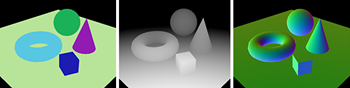
\includegraphics[width=4.85833in,height=1.21782in]{images/1_g_buffer.png}
		\caption{G-Buffer przedstawiający bufory koloru, głębi oraz wartości normalnych. \cite{tutsplus-deferred-2024}}
		\label{intro-deferred-shading}
	\end{figure}
	
	\item \textbf{Clustered shading}

	Znany także jako Forward+ lub Tiled Forward Rendering. Jest to nowa technika rysowania łącząca zalety Forward z optymalizacją pozwalającą na obsługę znacznie większej ilości świateł. Wykorzystuje do tego celu zależność, według której światła znajdujące się daleko od obiektów nie dostarczają wystarczającej ilości energii - a co za tym idzie światła -- aby poświęcać moc obliczeniową na ich wyliczanie. Pole widzenia dzielone jest na trójwymiarową siatkę klastrów o ustalonym rozmiarze. Następnie przechodząc w pętli po wszystkich światłach w scenie, określa które z nich mają wpływ na dany klaster, dodając je do listy świateł dla pola. Końcowym etapem jest rysowanie bardzo zbliżone do tradycyjnego Forward Rendering, lecz zamiast określania oświetlenia na podstawie wszystkich świateł w scenie określane jest ono jedynie na podstawie listy punktów światła, które mają wpływ na testowany punkt \cite{aortiz:clustered:2024}. Wizualizacja metody znajduje się na rys. \ref{intro-clustered-rendering}.

	Zaletą tej metody jest znaczne zmniejszenie ilości odczytów i zapisów do pamięci względem Deferred Shading z jednoczesnym zwiększeniem możliwości renderowania oświetlenia w porównaniu do klasycznego Forward Rendering. Nie rozwiązuje ona jednak problemu overdrawing'u, jedynie nieco go maskując. Do wydajnej pracy zalecana jest także obsługa Compute Shaders do wyliczania pokrycia klastrów przez oświetlenie, co wyklucza szybkie działanie na starszych platformach.

	\begin{figure}[htbp]
		\centering
		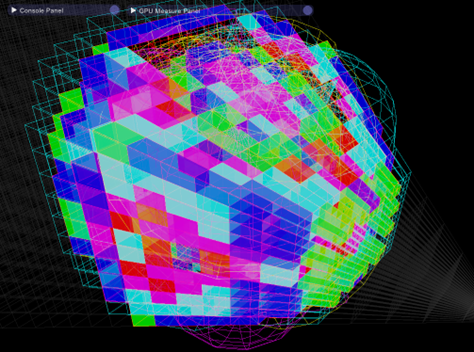
\includegraphics[width=4.94167in,height=3.67203in]{images/2_clustered_field.png}
		\caption{Podział pola widzenia na klastry. \cite{cnblogs:clustered:2024}}
		\label{intro-clustered-rendering}
	\end{figure}

	\item \textbf{Path Tracing}
	
	Technika śledzenia promieni (ang. Ray Tracing) jest najbardziej zbliżona do fizycznego modelu działania światła, co pozwala na uzyskanie bardzo realistycznych efektów. Z każdego punktu światła wysyłane są promienie światła, odbijając się od powierzchni obiektów, akumulując przy tym informacje o kolorze. Taki promień trafiając w sensor kamery przekazuje te informacje, które ostatecznie zostają zapisane na obraz docelowy. Taki model określa się mianem \emph{\textbf{Forward Path Tracing}}.
	
	Z perspektywy rysowania grafiki taka technika jest bardzo kosztowna obliczeniowo, gdyż zdecydowana większość promieni nie trafi do kamery, a zostanie rozproszona. W tym celu wykształciła się zoptymalizowana wersja techniki zwana \emph{\textbf{Backward Path Tracing}}. Różnica względem wariantu Forward polega na tym, że promienie śledzone są od kamery do światła, a nie odwrotnie. Jest to możliwe dzięki zasadzie wzajemności zaproponowanej przez Hermana Helmholtz'a, która głosi, że promień światła i jego odwrotność doświadcza takiej samej drogi oraz zjawisk fizycznych. \cite{wiki:helmholtz:2024}
	
	Technika ta pozwala na uzyskanie fotorealistycznych obrazów przy względnie prostym modelowaniu efektów, takich jak cienie, odbicia, refrakcję, głębię ostrości, okluzję otoczenia, czy symulowanie światła odbitego. Użycie Path Tracing'u w czasie rzeczywistym było bardzo rzadkie ze względu na jego koszt obliczeniowy. W 2018 roku firma NVIDIA wypuściła na rynek karty graficzne z serii RTX, które dodały funkcjonalność akceleracji sprzętowej obliczeń związanych z wykrywaniem kolizji promieni. Od tego czasu coraz więcej gier zaczęło korzystać z tej techniki celem poprawy jakości wyświetlanej grafiki.
\end{itemize}

\section{Modele cieniowania}

W celu realistycznego oddania świata rzeczywistego konieczne jest jak najdokładniejsze oddanie zachowania promienii świetlnych. Jednocześnie należy pamiętać o możliwej minimalizacji narzutu obliczeniowego celem poprawy wydajności.

\begin{itemize}
	\item \textbf{Cieniowanie płaskie}

	Najprostszy i najszybszy sposób cieniowania powierzchni. Oświetlenie wyliczane jest dla każdego wielokąta modelu, a następnie nakładane jako kolor danego poligonu.
	
	Wymaga bardzo małego nakładu obliczeniowego. Efekt jest wyraźnie nierealistyczny, sprawiając wrażenie ostrych krawędzi, co widoczne jest na rys. \ref{intro-flat-shading}. Mimo to bardzo dobrze oddaje on zależności między wielokątami, co jest przydatne na przykład w programach do modelowania grafiki 3D.

	\begin{figure}[htbp]
		\centering
		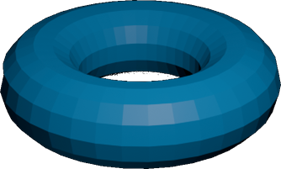
\includegraphics[width=3.90833in,height=2.34916in]{images/3_flat_shading_torus.png}
		\caption{Model torus'a narysowany przy pomocy cieniowania płaskiego.}
		\label{intro-flat-shading}
	\end{figure}

	\item \textbf{Cieniowanie Gouraud}
	
	Nazwana po autorze - Henri Gouraud -- technika cieniowania, w której natężenie światła wyliczane jest dla każdego wierzchołka, a następnie interpolowane dla fragmentów między tymi wierzchołkami. Charakteryzuje się niskim narzutem obliczeniowym i akceptowalnymi rezultatami. W przypadku modeli o niskiej rozdzielczości powoduje jednak powstawanie artefaktów, ze względu na kalkulacje oświetlenia jedynie dla wielokątów, których w takim przypadku jest niewiele, co widoczne jest na przykładowym obrazie widocznym na rys. \ref{intro-gouraud-shading}.

	\begin{figure}[htbp]
		\centering
		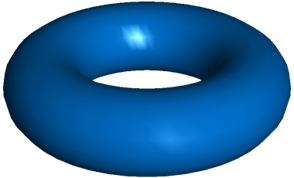
\includegraphics[width=4.08511in,height=2.475in]{images/4_gouraud_shading_torus.png}
		\caption{Model torus'a wygenerowany z użyciem cieniowania Gouraud i modelem światła Phong. \cite{wiki:gouraud:2024}}
		\label{intro-gouraud-shading}
	\end{figure}
	
	\item \textbf{Cieniowanie Phong}

	Model utworzony przez Bui Thong Phong na uniwersytecie Utah w 1973r. Poprawia niedokładność modelu Gouraud wykonując kalkulacje oświetlenia dla każdego fragmentu, a nie tylko wierzchołków. Efektem jest dobrze wyglądający model cieniowania pokazany na rys. \ref{intro-phong-shading}, z umiarkowanym kosztem obliczeniowym.
	
	Odbicia światła w tym modelu obliczane są na podstawie trzech parametrów widocznych na rys. \ref{intro-phong-components} - kolor otoczenia (ang. ambient), kolor rozproszony (ang. diffuse) używając modelu Lambertowskiego oraz tzw. specular reflection, obejmujący najjaśniejsze punkty odbite blisko lustrzanie.

	\begin{figure}[htbp]
		\centering
		
\includegraphics[width=3.45833in,height=2.08328in]{images/5_phong_shading_torus.png}
		\caption{Model torus'a wygenerowany z użyciem modelu cieniowania Phong.}
		\label{intro-phong-shading}
	\end{figure}
	
	\vfill
	\clearpage
	
	\begin{figure}[htbp]
		\centering
		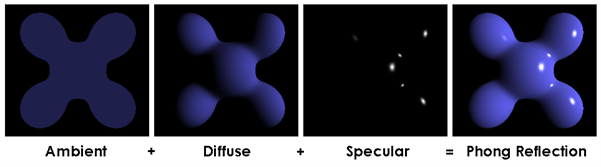
\includegraphics[width=6.25833in,height=1.74167in]{images/6_phong_shading_components.png}
		\caption{Komponenty składowe modelu Phong. \cite{wiki:phong:2024}}
		\label{intro-phong-components}
	\end{figure}
	
	\item \textbf{Model Blinn-Phong}
	
	Bazowy model Phong oblicza odbicia lustrzane (specular) poprzez wyznaczanie kąta między promieniem odbitym, a kamerą go obserwującą. Kąt ten jest następnie podstawiany do funkcji \emph{cos}, a wynik ograniczany do wartości z przedziału \textless0, 1\textgreater. Taki sposób kalkulacji ma jednak swoją wadę. W przypadku kątów większych od 90 stopni, wartość funkcji przyjmuje zawsze 0, co w przypadku bardzo chropowatych powierzchni może powodować artefakty, objawiające się jako twarde „odcięcie'' światła.
	
	Aby naprawić ten problem powstał model \emph{\textbf{Blinn-Phong}} zaproponowany przez James'a Blinn'a. Zamiast przeliczać bezpośrednio kąt odbicia do kąta kamery wyliczany jest wpierw kąt połowiczny między kątem padania światła i kątem obserwatora. Dzięki takiej modyfikacji oświetlenie zachowuje się bardziej naturalnie, bez znaczącego zwiększenia narzutu obliczeniowego.

	Model Blinn-Phong jest używany do obliczania odbić światła w starszych wersjach OpenGL i Direct3D używających \emph{Fixed Function Pipeline}.
	
	Różnice w obrazie wynikowym dla obu podejść można zobaczyć na rys. \ref{intro-phong-vs-blinn-phong}.
	
	\begin{figure}[htbp]
		\centering
		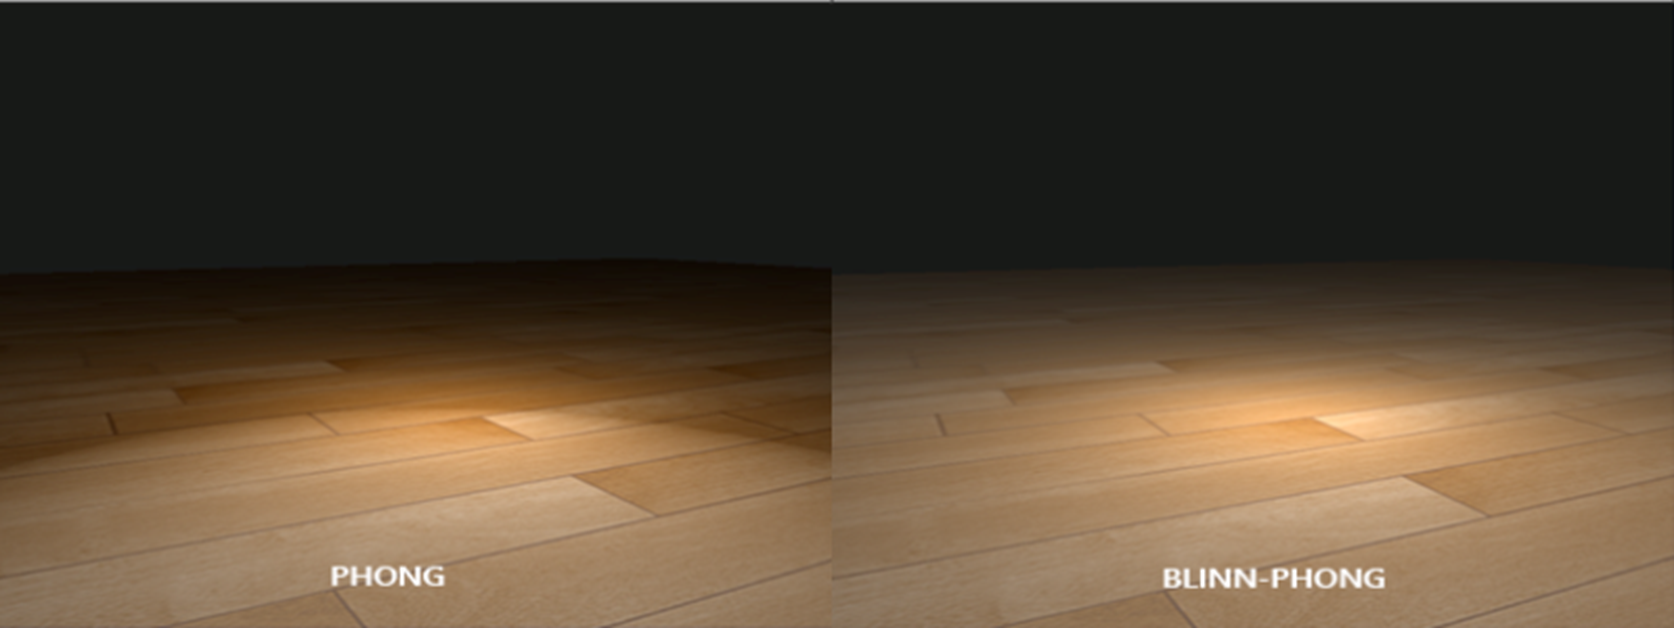
\includegraphics[width=5.58056in,height=2.09271in]{images/7_phong_vs_blinn_phong.png}
		\caption{Porównanie modelu Phong oraz Blinn-Phong dla bardzo chropowatej powierzchni i dużego kąta padania światła. \cite{learnopengl:advlighting:2024}}
		\label{intro-phong-vs-blinn-phong}
	\end{figure}
	
	\item \textbf{Physically Based Rendering}
	
	W skrócie \textbf{PBR}. Jest to grupa technik modelujących kalkulacje świetlne na podstawie prawdziwych zjawisk fizycznych. Ich niewątpliwą zaletą jest możliwość modelowania materiałów przy pomocy fizycznych właściwości obiektów bez uciekania się do sztuczek i aproksymacji.
	
	Systemy PBR najczęściej opierają się na modelu mikropowierzchni. Model taki aproksymuje zachowanie światła na mikroskopijnych nierównościach powierzchni obiektów. W przypadku równych materiałów światło będzie odbijało się w sposób bliski lustrzanemu, a chropowate powierzchnie będą je rozpraszać \cite{learnopengl:pbr:2024}, co widoczne jest na załączonym rys. \ref{intro-PBR}. Jest to zachowanie zbliżone do parametru chropowatości w opisanych wcześniej modelach.

	Drugim ważnym elementem systemu spełniającego założenie bazującego na rzeczywistości jest zasada zachowania energii. Ilość światła odbitego (a dokładniej jego energii) nie może przekraczać ilości włożonej energii. \cite{learnopengl:pbr:2024}

	Trzecim i ostatnim ważnym elementem opisywanego modelu jest funkcja typu BRDF (ang. Bidirectional Reflective Distribution Function). Przyjmuje ona jako parametry kierunek promienia światła \emph{\textbf{w\textsubscript{i}},} kierunek odbitego światła \emph{\textbf{w\textsubscript{o}}}, wektor normalny powierzchni \emph{\textbf{n}} oraz parametr \emph{\textbf{a}}, opisujący chropowatość powierzchni. Funkcja BRDF(w\textsubscript{i}, w\textsubscript{o}, n, a) aproksymuje ilość światła odbitego od powierzchni na podstawie jej parametrów \cite{learnopengl:pbr:2024}. Na przykład dla powierzchni lustra funkcja taka będzie zwracać 1 w przypadku kąta \emph{w\textsubscript{o}} będącego odbiciem \emph{w\textsubscript{o}}, a 0 w przeciwnym przypadku.
	
	\begin{figure}[htbp]
		\centering
		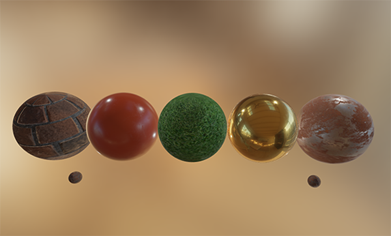
\includegraphics[width=5.425in,height=3.2752in]{images/8_pbr_surfaces.png}
		\caption{Powierzchnie cegły, plastiku, trawy, złota oraz zardzewiałego metalu wymodelowane przy pomocy PBR. \cite{learnopengl:pbr:2024}}
		\label{intro-PBR}
	\end{figure}
\end{itemize}

\section{Efekty graficzne poprawiające jakość obrazu}

Silniki renderujące oparte o klasyczne metody rysowania zmuszone są aproksymować zaawansowane efekty ze względu na ograniczenia tych metod. Poniżej opisane zostało kilka najpopularniejszych sposobów na poprawę jakości obrazu wynikowego.

\begin{itemize}
	\item \textbf{Wygładzanie krawędzi}

	Zjawisko \emph{\textbf{Aliasingu}} spowodowane jest ograniczeniami w metodach rasteryzacji obrazu przez karty graficzne. Wynika on z faktu, iż kolor pixeli na ekranie określany jest z odrębnych i nieciągłych punktów, czego efektem są ostre przejścia kolorów rysowanych obiektów i wrażenie „ząbkowania'' takich krawędzi.
	
	\item \textbf{MSAA}
	
	Najpopularniejszą metodą antialiasing jest \emph{\textbf{MSAA}} (ang. Multi-Sampling Anti Aliasing), czyli wielokrotne próbkowanie, której mechanizm działania został przedstawiony na rys. \ref{intro-msaa}. Jest to metoda akcelerowana sprzętowo przez współczesne karty graficzne, która jak nazwa wskazuje polega na wielokrotnym próbkowaniu z przesunięciem każdego pixela obrazu, a następnie wyciągania średniej jako ostatecznego koloru danego punktu. Technika ta wykazuje się dobrą jakością, ale jest względnie kosztowna obliczeniowo i nie jest możliwa w przypadku używania Deferred Shading.
	
	\begin{figure}[htbp]
		\centering
		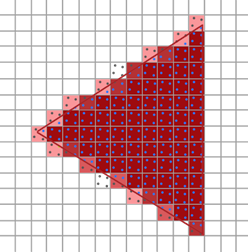
\includegraphics[width=3.4483in,height=3.5in]{images/9_MSAA_grid.png}
		\caption{Siatka reprezentująca działanie MSAA. Na niebiesko zaznaczone są punkty próbkowania, a czerwonymi liniami pokazane są krawędzie rysowanego obiektu. \cite{learnopengl:antialiasing:2024}}
		\label{intro-msaa}
	\end{figure}

	\item \textbf{TAA}
	
	\emph{\textbf{TAA}} (ang. Temporal Anti-Aliasing) jest uwspółcześnioną wersją MSAA. Zamiast wielokrotnego próbkowania pojedynczej klatki obrazu odbywa się ono na przestrzeni wielu, postępujących po sobie obrazach. Każdy proces rysowania rysuje obraz z lekkim przesunięciem punktów próbkowania pixeli, które następnie są uśredniane na potrzeby finałowego obrazu. Niewątpliwą zaletą tej techniki jest ograniczenie kosztu obliczeniowego, gdyż nie jest już wymagane wielokrotne próbkowanie pixeli. Pozwala ona także na użycie efektów \emph{dithering'u} do przezroczystości ze zmniejszoną ilością artefaktów. Z wad można wymienić narzut pamięci spowodowany koniecznością zapamiętywania poprzednich klatek, artefakty graficzne w postaci tzw. \emph{ghosting'u}, czyli pozostałości poprzednich klatek, a także widoczna nieostrość wynikowego obrazu.
	
	\item \textbf{FXAA}
	
	\emph{\textbf{FXAA}} (ang. Fast Aproximate Anti-Aliasing) operuje jako efekt post-procesowy w ścieżce generowania obrazu. Opracowany przez NVIDIA algorytm przetwarza obraz przez filtr górnoprzepustowy, wykrywając w ten sposób fragmenty obrazu o wysokim kontraście. Następnie metodami heurystycznymi znajduje w tych fragmentach krawędzie, które rozmywa przy pomocy kernel'a 3x3. Zaletą tej metody jest bardzo wysoka wydajność i brak narzutów pamięciowych. Jest to niestety też metoda dająca najsłabsze metody z wymienionych, powodując bardzo wyraźne rozmycie obrazu.
	
	\item \textbf{Odbicia środowiska}
	
	Aby dodać metalicznym i odbijającym światło obiektom głębi, należy dodać do silnika funkcjonalność obliczania odbić środowiskowych. Do najpopularniejszych metod należą:

	\item \textbf{Mapowanie sześcianów}

	Z angielskiego \emph{\textbf{Cube mapping}} jest techniką mapowania środowiskowego wykorzystującą do tego celu teksturę, zawierającą widok przestrzenny w 6 kierunkach, której przykładem jest rys. \ref{intro-cubemap}. Tekstura taka może być przygotowana z góry, z uwzględnieniem statycznych obiektów lub generowana w czasie rzeczywistym poprzez rysowanie geometrii z odpowiednich perspektyw. Tak przygotowany obraz nakładany jest następnie na rysowane obiekty w formie odbicia, co daje złudzenie realistycznego zjawiska.
	Taka metoda posiada jednak wiele wad. Generowanie sześciu obrazów co każdą klatkę prezentacji generuje bardzo wysokie koszty obliczeniowe. Można je zminimalizować zmniejszając jakość generowanego obrazu lub przeliczając jedynie kilka ścian na klatkę, ale zmniejsza to w efekcie jakość finalnego renderu. Przygotowane wcześniej cubemap'y omijają problemy z wydajnością, ale są z założenia statyczne, więc nie reprezentują zmian w otoczeniu. Dodatkowym ograniczeniem tej metody jest ograniczona dokładność odbić ze względu na różnice w generowanych mapach dla obiektów w różnych miejscach w przestrzeni. Sposobem obejścia tego problemu jest generowanie osobnych map dla różnych pomieszczeń bądź obiektów, ale wiąże się to z oczywistym narzutem obliczeniowym.
	
	\vfill
	\clearpage
	
	\begin{figure}[htbp]
		\centering
		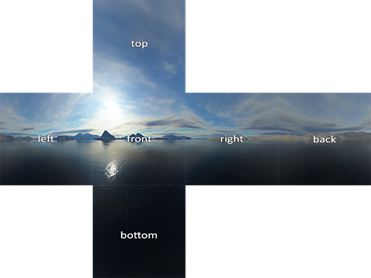
\includegraphics[width=5.14673in,height=3.85833in]{images/10_cubemap_environment.png}
		\caption{Przykład cubemap'y przedstawiającej tło środowiskowe.}
		\label{intro-cubemap}
	\end{figure}

	\item \textbf{Odbicia w przestrzeni ekranu}

	Z angielskiego \emph{\textbf{Screen-Space Reflection}} lub \emph{\textbf{SSR}}. Technika ta wychodzi z założenia, że większość odbić dotyczyć będzie obiektów, które zostały już wyrysowane, więc nie ma potrzeby renderowania ich po raz kolejny. W ten sposób ominąć można ograniczenia cubemap z jednoczesnym zachowaniem dostatecznej wydajności.

	Implementacja polega na wykonaniu pojedynczego śledzenia promienia w przestrzeni ekranu. Przyjmuje ona jako wejście bufory z teksturami kolorów, głębi oraz mapy odbijalności materiałów. Dla każdego fragmentu wykonuje pojedyncze śledzenie promienia na podstawie mapy głębi. Jeśli promień trafi na obiekt widoczny na ekranie, wykonywane jest jego odbicie, które następnie samplując po kolei z mapy głębi jest śledzone aż do trafienia obiektu. Jeśli tak się stanie, kolor trafionego materiału zostaje dodany jako odbicie do wyznaczanego koloru fragmentu. W przeciwnym wypadku za kolor odbity uznaje się światło nieba.
	Dużą zaletą tej techniki jest bardzo wysoka jakość odbić porównywalna do Ray-Tracing'u, szczególnie na płaskich powierzchniach pod dużym kątem, takich jak płaskie podłogi, czy powierzchnia wody. Z wad wymienić należy spory nakład obliczeniowy, a także artefakty, które powstają jeśli odbity promień trafi na obiekt nieznajdujący się w narysowanym obrazie.

	Przykład działania techniki został pokazany w ramach rys. \ref{intro-ssr}.

	\vfill
	\clearpage

	\begin{figure}[htbp]
		\centering
		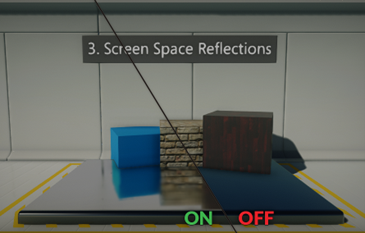
\includegraphics[width=5.06667in,height=3.2316in]{images/11_screen_space_reflections.png}
		\caption{Przykład działania Screen Space Reflections w porównaniu z brakiem tego efektu. \cite{flaxengine:ssr:2024}}
		\label{intro-ssr}
	\end{figure}

	\item \textbf{Ray Tracing}

	Najbardziej kosztowna wydajnościowo z opisywanych technik, ale dająca także najlepsze rezultaty, możliwe do zobaczenia na rys. \ref{intro-rt}. Opisana we wcześniejszym punkcie o Path Tracing'u metoda pozwala niskim kosztem dodatkowym uzyskać realistyczne odbicia bez ograniczeń \emph{SSR}. Podczas śledzenia promieni zliczany jest kumulowany kolor, co pozwala na uzyskanie odbić wielokrotnych, a także na rysowanie w odbiciach obiektów, które nie znajdują się na ekranie.

	\begin{figure}[htbp]
		\centering
		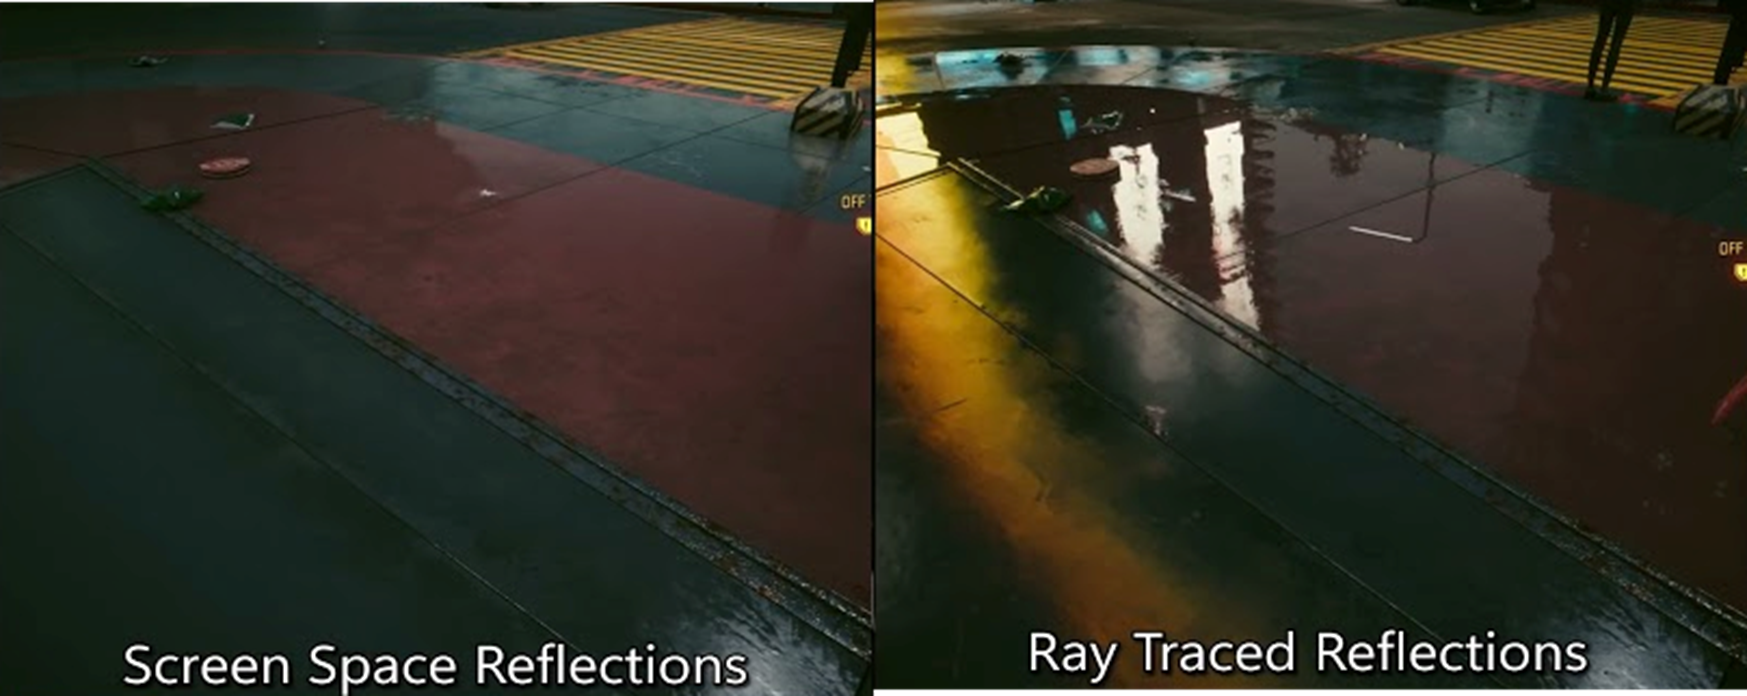
\includegraphics[width=5.82534in,height=2.32148in]{images/12_ssr_vs_rt.png}
		\caption{Porównanie Screen Space Reflections z odbiciami uzyskanymi techniką śledzenia promieni. \cite{niktek:reflections:2024}}
		\label{intro-rt}
	\end{figure}
	
	\vfill
	\clearpage
	
	\item \textbf{Ambient Occlusion}
	
	Okluzja otoczenia (ang. \emph{\textbf{Ambient Occlusion}}) jest techniką symulowania ograniczonej dostępności rozproszonego światła do kątów i zakamarków obiektów. Pozwala to na uzyskanie realistycznie wyglądającej aproksymacji prawdziwego zachowania światła.

	Do najpopularniejszych implementacji należą \emph{\textbf{SSAO}} (ang. Screen Space Ambient Occlusion), działający podobnie do \emph{SSR} oraz Path Tracing, który symuluje ten efekt symulując fizyczne zachowanie światła.
\end{itemize}

\section{Optymalizacja rysowania}

Poza dobrą jakością, bardzo istotnym elementem dobrego silnika renderującego jest także odpowiednia wydajność. Większość opisanych w poprzednim punkcie technik wyraźnie obciąża komputer rysujący, co zmusza do zastosowania technik optymalizacyjnych celem uzyskania dostatecznej szybkości działania. Poniżej opisane zostało kilka przykładowych, najczęściej stosowanych technik.

\begin{itemize}
	\item \textbf{Batching}

	Jednym z ograniczeń wydajności rysowania jest tzw. context switching, czyli zmiana używanego do rysowania shader'a i/lub materiału, a także ilość zapytań rysowania wysyłanych do karty graficznej. Aby zmniejszyć narzut wydajnościowy spowodowany takimi zmianami stosuje się technikę grupowania, czyli \emph{\textbf{Batching}}.
	Metoda ta dzieli się przede wszystkim na grupowanie statyczne i dynamiczne. Pierwsze wyliczane jest jeszcze przed uruchomieniem programu i dotyczy obiektów statycznych. Łączone są one w jeden, duży model i tak wysyłane w jednym zapytaniu do karty graficznej. Odmiana dynamiczna odbywa się przy rysowaniu w czasie rzeczywistym i sprowadza się do grupowania obiektów używających tego samego materiału do rysowania bezpośrednio po sobie, co pozwala uniknąć kosztownych zmian kontekstu. Metoda ta słabo nadaje się do obiektów używających różnych materiałów, gdyż wymagałoby to dostosowywania programów cieniujących do obsługi takiej techniki. Zupełnie brak jest możliwości łączenia ze sobą obiektów używających różnych shader'ów.

	\item \textbf{Frustum culling}

	Nie wszystkie obiekty sceny są widoczne w renderowanym jej fragmencie. Część znajduje się poza obszarem kamery, część jest zasłonięta przez wzgórza czy inne obiekty. W takim przypadku zbędną jest próba rysowania takich powierzchni, marnująć jedynie moc obliczeniową. Na pomoc wychodzi technika zwana \emph{\textbf{Frustum culling}}, pomijająca rysowanie niewidocznych obiektów na podstawie systemu wykrywania kontaktu ze stożkiem pola widzenia.
	Technika ta dzieli się na dwa zasadnicze podtypy. Pierwszym z nich, wykorzystywany klasycznie w silnikach idTech oraz Valve Source jest typ statyczny. W trakcie kompilacji mapy wyliczane są punkty widoczności na całej mapie, tak aby można było określić jakie fragmenty mogą być widoczne, a jakich nie trzeba rysować. Zaletą takiego rozwiązania jest bardzo wysoka wydajność, ale ograniczona jest ona do korytarzowej struktury pomieszczeń, gdyż na otwartych przestrzeniach ciężko mieć pewność co do widoczności w statycznej kalkulacji.
	Drugim sposobem jest typ dynamiczny. Przed rysowaniem klatki obrazu kalkulowane jest pokrywanie się obiektów sceny z fragmentem widocznym przez kamerę. Ze względu na wysoki koszt porównywania pełnych obiektów wykorzystuje się tzw. \emph{\textbf{Bounding Volumes}}, czyli figury geometryczne aproksymujące przestrzeń zajmowaną przez obiekt. Do najczęściej używanych należą sfery, prostopadłościany wyrównane do osi (AABB), czy prostopadłościany z rotacjami (OBB).
	W przypadku bardzo dużej ilości obiektów koszt obliczania elementów do narysowania wciąż może być zbyt duży. W tym celu wdrożyć można strukturę drzewową zwaną \emph{\textbf{Space partitioning}}, która dzieli rekursywnie przestrzeń na podfigury z informacją o ilości zawartych w nich obiektów. Następnie sprawdzając kolizje struktura taka umożliwia przejście „w dół'' drzewa, wykonując mniejszą ilość kalkulacji intersekcji. Najczęściej używa się drzewa z czterema podelementami dla gier 2D, ośmioma dla gier 3D, lub struktury \emph{\textbf{BSP}} (Binary Space Partitioning) jako optymalizacji dla większej ilości obiektów. System BSP używany jest we wspomnianych silnikach idTech oraz Valve Source.
	
	\item \textbf{Poziom detali}
	
	Z angielskiego \emph{\textbf{Level of Detail}} generuje dla każdego modelu jego alternatywne warianty ze zmniejszoną dokładnością i/lub ilością detali. W czasie rzeczywistym modele są podmieniane na niższej jakości wraz ze zwiększaniem się dystansu od kamery, co pozwala na uniknięcie rysowania nadmiernej ilości wielokątów w sytuacjach, w których użytkownik ma małą szansę ich zauważenia.
	
	\begin{figure}[htbp]
		\centering
		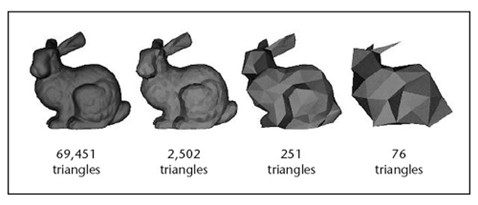
\includegraphics[width=4.975in,height=2.13971in]{images/13_LOD_rabbit.jpg}
		\caption{Poziom detali przedstawiony na modelu królika. \cite{3dstudio:lod:2024}}
	\end{figure}
\end{itemize}

\section{API graficzne}

Wydajny system renderujący powinien używać do rysowania akceleracji sprzętowej w postaci kart graficznych. W tym celu zalecanym jest użycie jednego ze wspieranych przez platformę API graficznych, które pozwalają na uzyskanie zamierzonego efektu bez konieczności dostosowywania kodu do konkretnych implementacji czy sprzętu. Wybór interfejsu powinien zależeć od zastosowania. Aplikacje celujące w starsze systemy będą miały odmienne wymagania do programów wyspecjalizowanych pod najszybsze komputery i najlepszą jakość grafiki. Nowsze API z reguły pozwalają na większą kontrolę nad procesem rysowania, ale kosztem złożoności ich użycia, a co za tym idzie czasem produkcji i skomplikowaniem korzystających z nich programów. Poniżej przedstawione zostało kilka przykładowych interfejsów.

\begin{itemize}
	\item \textbf{DirectX}

	Interfejs stworzony przez Microsoft dla platformy Windows i dokładniej opisany w następnym rozdziale. Jego najnowsza wersja -- DirectX 12 -- wspiera najnowsze rozszerzenia graficzne, takie jak DXR (DirectX RayTracing), VRS (Variable Rate Shading), Mesh Shaders czy DirectStorage.
	
	\item \textbf{OpenGL}

	Zaprojektowany w latach 90 przez Silicon Graphics stał się de facto standardem w dziedzinie interfejsów graficznych. Działa na zasadzie maszyny stanów, w której stan zapisywany jest po stronie sterownika graficznego. W pierwotnym wydaniu działający na zasadzie \emph{\textbf{Fixed Function Pipeline}}, a od wersji 3.1 opierający całe swoje działanie na modyfikowalnych ścieżkach rysowania. Najnowsza wersja to OpenGL 4.6. Wszystkie popularne systemy operacyjne wspierają ten standard z wyłączeniem Apple MacOS, który obsługuje jedynie do wersji OpenGL 4.1.

	\item \textbf{Vulkan}
	
	Sukcesor OpenGL zaprojektowany przez grupę Khronos. Względem swojego poprzednika rozszerza wsparcie o nowsze technologie, obsługę wielowątkowości oraz bardziej strukturalną konstrukcję. W dobrych rękach pozwala także na zmniejszenie narzutu obliczeniowego na procesor, a także zwiększenie wydajności renderowania poprzez możliwość określania przekazania sterownikowi bardziej dokładnych założeń co do modeli czy tekstur.
\end{itemize}

\section{Istniejące silniki graficzne}

Ze względu na duże zapotrzebowanie na rynku na różnego rodzaju programy do wyświetlania grafiki 2D i 3D, powstało wiele implementacji tego typu modułów. Część z nich można wykorzystać jako niezależne moduły renderujące, a część jest zintegrowana z konkretnym silnikiem graficznym bądź programem go wykorzystującym.

\begin{itemize}
	\item \textbf{Blender EEVEE}

	Stworzony na potrzeby programu do modelowania graficznego Blender silnik renderujący z założeniem działania w czasie rzeczywistym. Do rysowania grafiki korzysta z API OpenGL.

	Wspiera między innymi kalkulacje cieni metodami klasycznymi oraz przy pomocy Ray Tracing'u, oświetlenie wolumetryczne, oświetlenie globalne przy pomocy RT, a także efekty Post Process w postaci głębi ostrości, rozmycia w ruchu, czy Tonemapping'u z HDR do SDR.

	Przykład obiektu narysowanego przy pomocy EEVEE został pokazany na rys. \ref{intro-eevee}.

	\begin{figure}[htbp]
		\centering
		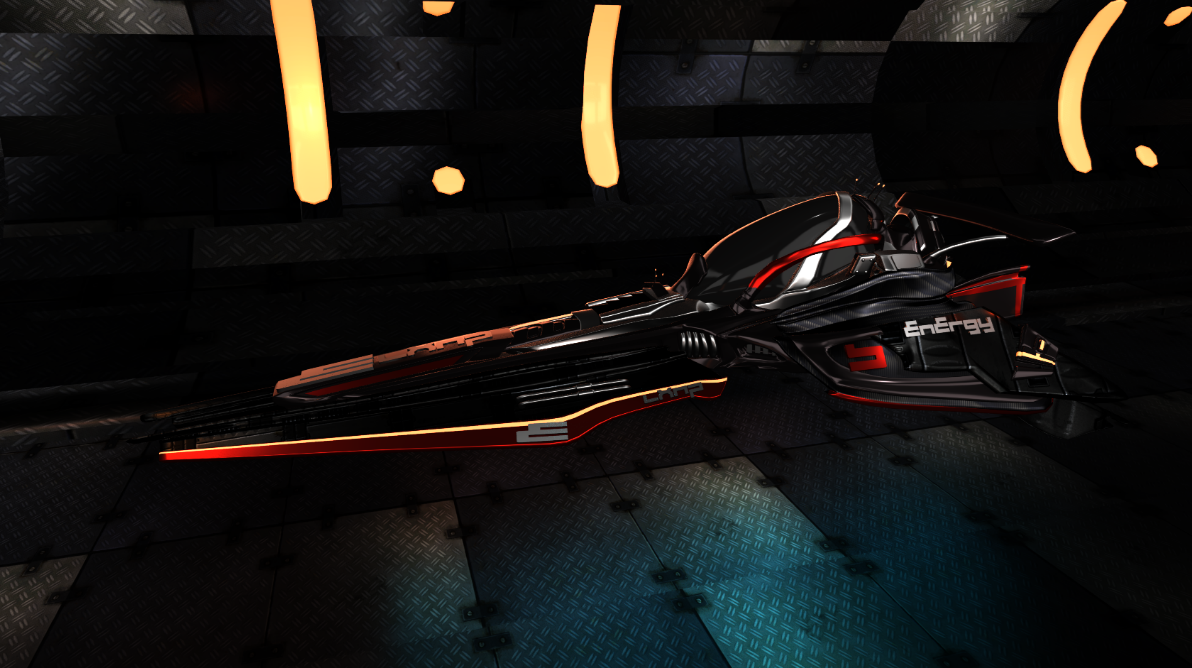
\includegraphics[width=5.41667in,height=3.03651in]{images/14_eevee.png}
		\caption{Obraz wygenerowany przy pomocy silnika EEVEE w programie Blender 4.2.1.}
		\label{intro-eevee}
	\end{figure}

	\item \textbf{Blender Cycles}

	Bardziej zaawansowany od EEVEE moduł stworzony z myślą o generowaniu fotorealistycznych renderów złożonej grafiki trójwymiarowej. Opiera swoje działanie na Path Tracing'u z wykorzystaniem akceleracji sprzętowej technologiami NVIDIA CUDA, NVIDIA OptiX, AMD HIP (RT), czy Intel oneAPI. Ze względu na charakterystykę algorytmu Path Tracing'u renderowanie z użyciem tego silnika wymaga bardzo dużej mocy obliczeniowej. W przeciwnym wypadku konieczne jest zmniejszenie ilości próbek dla każdego pixela, co powoduje ziarnistość obrazu wynikowego, widocznego na rys. \ref{intro-cycles-low}. Pomóc może dostępny w module system odszumiania obrazu.

	\vfill
	\clearpage

	\begin{figure}[htbp]
		\centering
		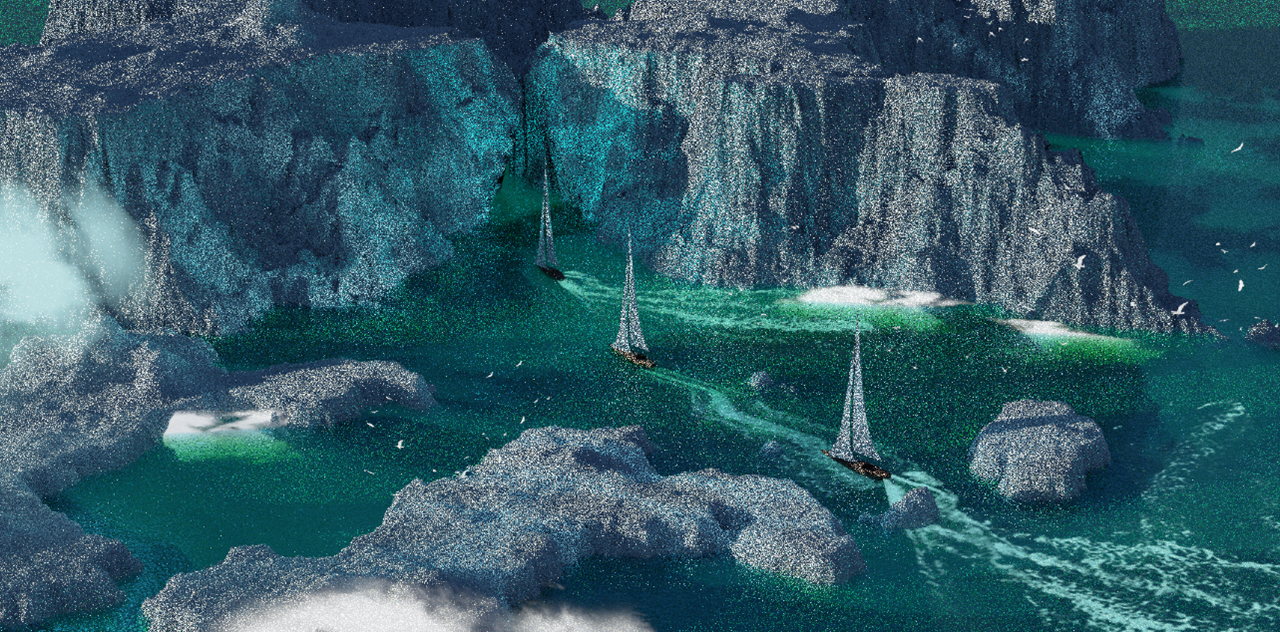
\includegraphics[width=5.81975in,height=2.875in]{images/15_cycles_low_samples.png}
		\caption{Obraz wygenerowany przez Cycles z niską ilością próbek, a przez to widocznym zaszumieniem.}
		\label{intro-cycles-low}
	\end{figure}

	Dzięki zastosowaniu metody śledzenia promieni do generowania obrazu, Cycles jest zdolny do generowania grafiki o bardzo wysokiej jakości i złożoności. Moduł ten poza funkcjami przejętymi od EEVEE posiada między innymi także pełną obsługę rozszerzonego standardu PBR, refrakcji i odbić światła, miękkich cieni, rozszerzonego globalnego oświetlenia w oparciu o system RT, przezroczystości, czy efektów wolumetrycznych także opartych o śledzenie promieni. Poprawnie wyrenderowany przy pomocy Cycles obraz został pokazany na rys. \ref{intro-cycles-high}.

	\begin{figure}[htbp]
		\centering
		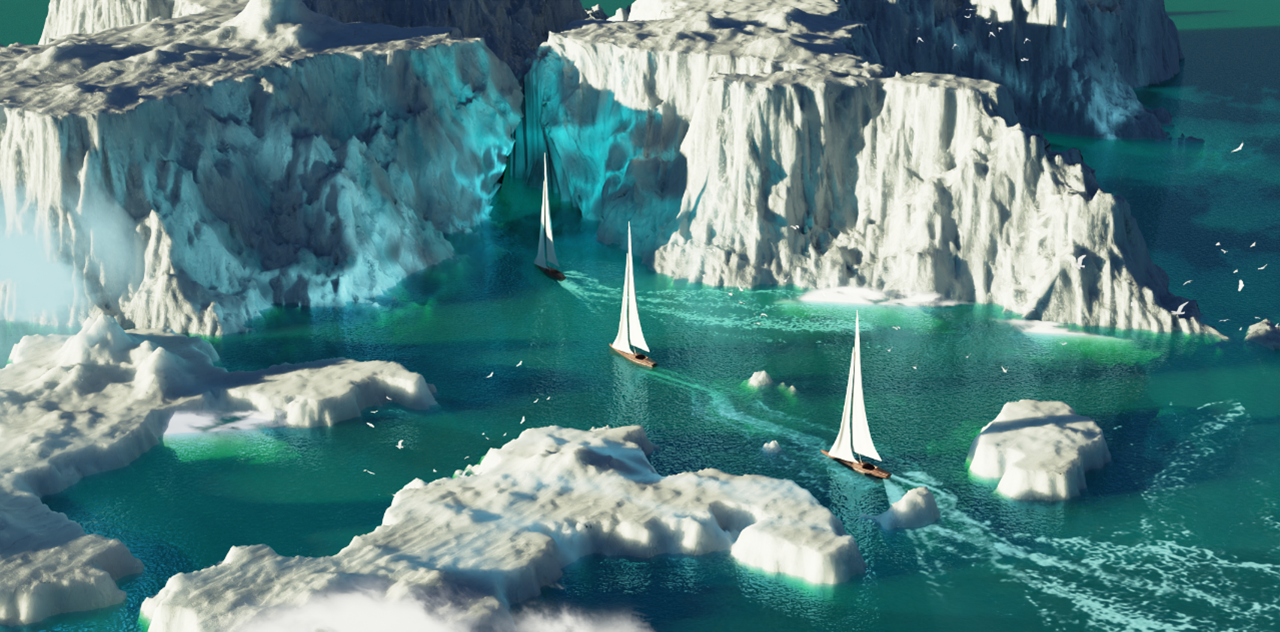
\includegraphics[width=5.81974in,height=2.875in]{images/16_high_samples.png}
		\caption{Obraz wygenerowany przez Cycles w programie Blender 4.2.1.}
		\label{intro-cycles-high}
	\end{figure}

	\vfill
	\clearpage

	\item \textbf{Unreal Engine}
	
	Silnik renderujący zastosowany w Unreal Engine jest jednym z najlepszych jakościowo dostępnych na rynku. Pozwala on na generowanie bliskich fotorealizmowi grafik w czasie rzeczywistym do zastosowania w grach. Oparty na systemie Deferred Shading posiada wiele zaawansowanych technik optymalizujących rysowanie obrazu. Najbardziej znanymi z nich są Lumen oraz Nanite. Pierwszy jest częściowo akcelerowanym sprzętowo algorytmem oświetlenia globalnego, pozwalającego na uzyskanie bardzo dobrych jak na standardy czasu rzeczywistego efektów względnie niskim kosztem obliczeniowym. Nanite natomiast zastępuje system Level of Detail, generując w czasie rzeczywistym fragmenty modeli o odpowiedniej jakości. Pozwala to na uzyskanie bardzo wysokiej szczegółowości modeli bez utraty wydajności związanej z systemem LOD. Oprócz opisanych technologii specyficznych, Unreal Engine obsługuje także między innymi akcelerowany sprzętowo Ray Tracing do obsługi odbić, cieni oraz Lumen, pełną obsługę PBR, czy subsurface scattering. Dzięki zastosowaniu RHI (Render Hardware Interface) czyli interfejsu abstrakcji, UE5 pozwala na skorzystanie z DirectX 11 oraz 12, OpenGL, jak i Vulkan do akceleracji graficznej. Nie wszystkie funkcjonalności są jednak dostępne w starszych API. 
	
	Przykład obrazu wygenerowanego przy pomocy Unreal Engine można zobaczyć na rys. \ref{intro-unreal-engine}.

	\begin{figure}[htbp]
		\centering
		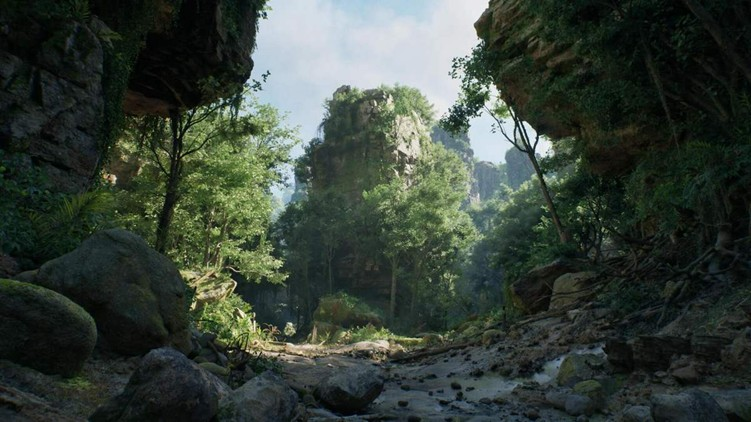
\includegraphics[width=5.21482in,height=2.93333in]{images/17_Unreal_engine_5_2.jpg}
		\caption{Klatka obrazu wygenerowana przez Unreal Engine 5.2.}
		\label{intro-unreal-engine}
	\end{figure}

	\item \textbf{Godot}

	W przeciwieństwie do większości popularnych silników graficznych, Godot nie korzysta z rysowania typu Deferred. Zamiast tego wykorzystywana jest technika Clustered Forward Rendering \cite{godot:rendererdesign:2024}. Technika ta została zastosowana ze względu na platformy docelowe opisywanego silnika, którymi są głównie mniej wydajne urządzenia mobilne, jak i uruchamianie aplikacji w przeglądarce przy użyciu WebGL.
	Architektura modułu także jest nieco odmienna od pozostałych. Jest on odrębnym podsystemem komunikującym się z głównym silnikiem jedynie poprzez pojedyncze gniazdo komunikacji. Przyjmuje jako argumenty parametry konfiguracyjne i strukturę opisującą scenę wraz z unikatowymi ID obiektów. Taka konstrukcja zmniejsza co prawda kontrolę programistów nad procesem rysowania, ale znacznie ułatwia rozwijanie kodu odpowiedzialnego za rysowanie. Ułatwia to także wsparcie dla różnych API graficznych.

	Silnik renderujący Godot posiada obsługę większości współczesnych efektów graficznych, takich jak Ambient Occlusion, Subsurface Scattering, Screen Space Reflections, czy efekty Post Process typu głębi ostrości, bądź rozmycia w ruchu. Moduł posiada także obsługę materiałów opartych o PBR. Nie celuje on jednak w wysoki fotorealizm, a bardziej w przystępną wydajność na słabszych urządzeniach. Przykładowym renderem za pomocą silnika Godot jest rys. \ref{intro-godot}.

	\begin{figure}[htbp]
		\centering
		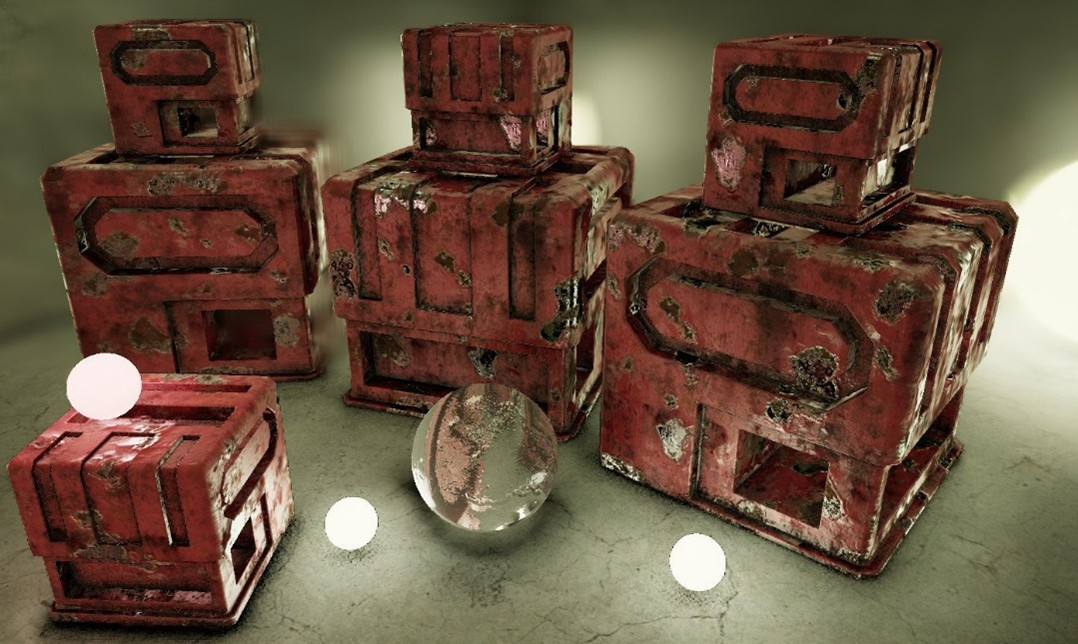
\includegraphics[width=4.90152in,height=2.92893in]{images/18_Godot_3_example.jpg}
		\caption{Klatka obrazu wygenerowana przez silnik Godot 3. \cite{godot:rendererdesign:2024}}
		\label{intro-godot}
	\end{figure}
\end{itemize}
    \chapter{Direct3D}

W latach 90 Microsoft prowadził transformację z systemu MS-DOS na nowo
powstały system Windows. Ze względu na duże zmiany w architekturze
między tymi systemami portowanie aplikacji okazało się być bardzo
utrudnione, a niejasna budowa i wsparcie API graficznych Windows
odstraszała potencjalnych deweloperów gier i programów multimedialnych.

Microsoft zareagował na ten problem dodając wsparcie dla API OpenGL do
system Windows. Nie było to jednak rozwiązanie idealne. Firma chciała
przejąć pełną kontrolę nad swoim systemem, oferując jednocześnie
rozwiązania niebędące częścią specyfikacji konkurencji. W ten sposób
narodził się standard DirectX, którego najważniejszy komponent --
Direct3D -- miał konkurować ze standardem od Silicon Graphics.

W przeciwieństwie do swojego głownego rywala, DirectX został oparty o
architekturę COM (\emph{\textbf{Component Object Model}}), która pozwala
na deklarowanie obiektów w sposób neutralny językowo, oddzielnie od
implementacji.

DirectX, a co za tym idzie także Direct3D przechodziły wiele zmian na
przestrzeni lat. Pierwotna wersja zakładała użycie trybu
natychmiastowego (ang. \emph{Imeediate Mode}). Nowsze odsłony od wersji
10.0 opierają swoje działanie o listy komend i zunifikowany model
shader'ów, podobnie jak w przypadku OpenGL czy Vulkan. Wersja 8.0
wprowadziła rewolucję w postaci wsparcia shader'ów, które rozwinięte
zostało znacząco przy okazji 9.0 o obsługę języka HLSL. \cite{wiki:direct3d:2024}

Najnowszym wydaniem jest DirectX 12 wydany w 2015r. Swoją architekturą
odbiega wyraźnie od poprzednika -- DirectX 11 -- podchodząc do problemu
w sposób znacznie bardziej niskopoziomowy, oddając większą kontrolę
programistom kosztem złożoności obsługi.

% Usunięto puste lub zbędne sekcje enumerate

\section{Shader'y w Direct3D} % Zmieniono z enumerate

Direct3D 9.0 dodał wsparcie dla HLSL (ang. \emph{\textbf{High Level
		Shader Language}}), stworzonego przez Microsoft języka programowania
shader'ów, pozwalającego na pełną kontrolę nad prawie każdym etapem
ścieżki rysowania grafiki z wykorzystaniem tego API. Składnia HLSL jest
zbliżona do stworzonego przez NVIDIA języka Cg.

% Zmieniono itemize + quote na subsection dla lepszej struktury
\subsection{Vertex Shader}
Shader odpowiedzialny za transformację pozycji Vertex'ów, czyli punktów
w trójwymiarowej przestrzeni będących wierzchołkami rysowanych
wielokątów. Na tym etapie nakładane są przekształcenia różnych
przestrzeni, na przykład z przestrzeni modelu (ang. \emph{\textbf{model
		space}}) do przestrzeni świata (ang. \emph{\textbf{world space}}), a
kończąc na przestrzeni widoku (ang. \emph{\textbf{view space}}). Etap ten pozwala także na implementacje bardziej zaawansowanych technik,
takich jak deformowanie modeli na podstawie map wysokościowych,
modyfikacje kolorów, czy transformacje nałożonych na model tekstur.

\subsection{Tesselation Shader}
Wprowadzony w Direct3D 11. Pozwala na kontrolowanie procesu Teselacji,
czyli programowego zwiększanie ilości wielokątów, na przykład celem
wykorzystania przy technice map wysokościowych, czy dodatkowych
optymalizacjach systemu LOD.

\subsection{Geometry shader}
Programowalny od Direct3D 10. Kontroluje generowanie prymitywów
przekazywanych do procesu rasteryzacji, takich jak trójkąty, linie,
punkty, czy złożone wielokąty. Pozwala to na optymalizację rysowania
niektórych typów obiektów, przede wszystkim dwuwymiarowych sprite'ów czy
cubemap.

\subsection{Pixel shader}
Zwany także jako Fragment Shader w OpenGL. Odpowiada za wyliczanie
koloru pixela po rasteryzacji. Uwzględnia wartości przekazane z
poprzednich etapów, wyliczanie oświetlenia, cieniowania, nakładania
tekstur, przezroczystości i innych efektów związanych bezpośrednio z
kolorem powierzchni.

% Obraz wycentrowany wraz z podpisem
\begin{figure}[htbp] % Można dostosować specyfikatory położenia [htbp]
	\centering
	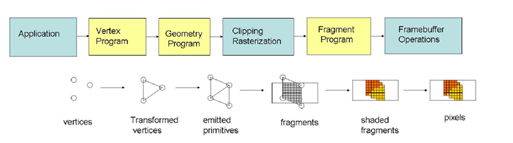
\includegraphics[width=5.34091in,height=1.48711in]{images/19_shader_pipeline.png}
	\caption{Wizualna reprezentacja kolejnych etapów rysowania przy pomocy shader'ów. \cite{researchgate:openglpipeline:2024}}
	\label{fig:shader_pipeline} % Dodano etykietę dla odniesień
\end{figure}

\subsection{Compute shader}
Konstrukcja współczesnych układów graficznych pozwala na ich
wykorzystanie poza dziedziną rysowania grafiki. Algorytmy korzystające z
szerokiej wielowątkowości i równoległości skorzystają także z
uruchamiania na GPU. Do tego celu stworzone zostały shader'y
przetwarzające (ang. \emph{\textbf{Compute Shader}}), wprowadzone przy
okazji Direct3D 11.

Programy takiego typu mogą, ale nie muszą być wykorzystywane jako pomoc
do generowania grafiki. Algorytmy kryptograficzne, rekonstrukcja skanów
tomogarfii komputerowej, przetwarzanie wideo, czy szczególnie dziś
powszechne uczenie maszynowe to tylko kilka przykładów wykorzystania
GPGPU (ang. \emph{\textbf{General Purpose Graphics Processing Unit}}) we
współczesnym świecie.

\subsection{Mesh shaders}
Ze względu na ewolucję sprzętową układów graficznych dotychczasowa
konstrukcja ścieżki rysowania przestała w optymalny sposób oddawać
niskopoziomowy sposób ich działania. Architektura SIMD (ang.
\emph{\textbf{Single Instruction Multiple Data}}) lepiej odpowiada
shader'om typu Compute, niż Vertex. Compute shaders mają niestety wadę w
postaci braku integracji z resztą pipeline'u renderowania, a co za tym
idzie konieczność zapisu i odczytu do pamięci głównej karty graficznej,
co wyraźnie spowalnia ich działanie. Z tego powodu Microsoft w DirectX 12 Ultimate wprowadził obsługę tzw.
\emph{\textbf{Mesh Shaders}}. Zastępują one pierwszą część ścieżki
rysowania, czyli Vertex, Geometry oraz Tesselation shaders i przekazują
swoje wyjście bezpośrednio do procesu rasteryzacji. Swoją konstrukcją
przypominają Compute shaders, lecz są zintegrowane bezpośrednio w
strumieniu danych rysowania klatki obrazu.

\section{Zaawansowane rozszerzenia Direct3D} % Zmieniono z enumerate

W czasie istnienia D3D układy graficzne i techniki rysowania obrazu
ewoluowały z prostego schematu \emph{Fixed Function Pipeline}, do
bardziej zaawansowanych, programowalnych shader'ów. Dodatkowe efekty
graficzne często wiązały się jednak z koniecznością dodatkowych
optymalizacji z uwzględnieniem sprzętowej akceleracji. Przedstawione
poniżej technologie są przykładami takich funkcji.

\subsection{WARP}
Skrót od \emph{\textbf{Windows Advanded Rasterization Platform}}. Jest
to programowy rasterizer pozwalający na uruchamianie aplikacji opartych
o Direct3D z użyciem rysowania programowego, bez akceleracji sprzętowej
układu graficznego. Wprowadzony w Windows 7 pierwotnie obsługiwał jedynie DirectX w wersji
10, współcześnie na systemie Windows 11 obsługuje pełny standard DirectX
12 Ultimate.

\subsection{Direct2D}
Interfejs programistyczny analogiczny do Direct3D, ale służący do
rysowania wektorowej grafiki dwuwymiarowej. Posiada wsparcie dla
rysowania przy pomocy CPU i GPU, krzywych Bezier'a, metod blending'u,
wypełniania i obrysowywania kolorem, a także rysowania sprite'ów. Najnowszym wydaniem jest Direct2D 1.3 wypuszczony wraz z Windows 10.

\subsection{DirectWrite}
Bardzo często wykorzystywaną funkcją, szczególnie w aplikacjach
użytkowych jest rysowanie tekstu. Funkcja taka przydaje się też często w
akcelerowanych sprzętowo silnikach rysujących interfejs aplikacji, bądź
jako nakładka interfejsu do gier. Proces renderowania wysokiej jakości i czytelności tekstu jest
skomplikowany. Z tego powodu powstało rozszerzenie DirectWrite, które
ułatwia ten proces. Z jego pomocą możliwe jest akcelerowane sprzętowo
rysowanie tekstu ze wsparciem Microsoft ClearType, czy OpenType. Do
działania wymagany jest system operacyjny Windows 7 lub wyżej.

\subsection{DirectX Ray-Tracing}
W skrócie \emph{\textbf{DXR}}. Wprowadzony w Direct3D 12 interfejs
akceleracji sprzętowej rozwiązań śledzenia promieni. Aplikacja uzupełnia
modelami nowo wprowadzoną strukturę drzewa, będącą akceleratorem
wykrywania kolizji promieni i wielokątów. Następnie przeprowadzane jest
śledzenie promieni, które przy odbiciach wywołuje nowe, specjalne
shader'y typu RT decydujące o sposobie odbicia i kolorze.

\subsection{DirectStorage}
Współczesne programy, a w szczególności gry potrzebują ogromnej ilości
zasobów wczytanych do pamięci układu graficznego. Proces ten jest
czasochłonny, ze względu na konieczność wczytania danych z nośnika,
dekodowania przez procesor centralny i wgrania na układ graficzny
najczęściej magistralą PCI-E. Firma Microsoft podjęła więc decyzję o stworzeniu API DirectStorage jako
część Direct3D 12. Pozwala ono na ominięcie CPU w procesie wczytywania i
odczyt danych bezpośrednio z nośnika typu SSD NVME do pamięci karty
graficznej. Obecnie nie jest to zbyt rozpowszechnione rozwiązanie, ale w
przyszłości może pozwolić na znaczące przyspieszenie wczytywania gier, a
nawet na zupełne wyeliminowanie ekranów ładowania.

\section{Alternatywne implementacje Direct3D na inne platformy.} % Zmieniono z enumerate

DirectX, a co za tym idzie Direct3D są interfejsami oficjalnie
wspieranymi jedynie na systemie Microsoft Windows. Jednak użytkownicy
innych systemów operacyjnych także chcieli mieć możliwość korzystania z
aplikacji napisanych w tym standardzie. Z tego powodu powstało kilka
implementacji standardu na systemy klasy Unix.

\subsection{DXVK}
Implementacja DirectX 8 do 11, będąca warstwą translacji między DirectX,
a Vulkan \cite{github:dxvk:2024}. Wspiera systemy Linux, a także możliwość uruchomienia
na systemie Windows. Posiada częściowe i nieoficjalne wsparcie dla
systemu Apple macOS. Jest częścią podsystemu Proton, będącego warstwą
kompatybilności opartą o moduł Wine pozwalającą uruchamiać gry i
aplikacje zgodne z API Windows na systemach Unix.

\subsection{VKD3D}
Moduł analogiczny do DXVK, ale pozwalający na uruchamianie aplikacji
zgodnych z DirectX 12. Posiada wsparcie dla systemów Linux i Windows. Najnowsze odsłony od wersji 2.11 posiadają wsparcie dla modułu DXR.

    \chapter{Architektura oraz założenia systemu}
Przed faktycznym rozpoczęciem prac nad złożonym systemem programowym należy najpierw zastanowić się nad jego architekturą.
Ułatwia to określenie wymagań, celów, a także potencjalnych trudności które można napotkać w trakcie prac. 

\section{Rodzaje systemów rysujących}
Głównym założeniem projektu jest stworzenie uniwersalnego, modularnego systemu rysującego.
Systemy tego typu przyjmują najczęściej formę, którą można określić jako punkt między dwoma ekstremami. 

\subsection{Moduł niezależny}
\label{Subsection_module_types_engine}
Po jednej stronie spektrum znajduje się system prawie całkowicie niezależny. Swoim działaniem jest zbliżony do silników do gier, gdzie skrypt klienta zostaje periodycznie wywołany w celu zmiany wewnętrznego stanu modułu. System jest w takim przypadku odpowiedzialny za większość kontroli przepływu programu, w tym operacji związanych z rysowaniem, inicjalizację okna, ruch kamery w odpowiedzi na interakcje z użytkownikiem, generowanie modelu 3D na podstawie pliku wejściowego, czy obliczanie zaawansowanych efektów świetlnych. Silnik przechowuje listę obiektów sceny wraz z ich parametrami, takimi jak translacja, materiał czy wzajemne relacje, które wykorzystuje do renderowania obrazu. 

Zastosowanie takiej metody zwiększa potencjał wydajnościowy silnika oraz wyraźnie zmniejsza nakład pracy dla programisty piszącego aplikację kliencką. Pozwala to także na potencjalną całkowitą niezależność od użytego API graficznego oraz systemu operacyjnego, gdyż możliwa jest realizacja w formie interfejsu, której implementacje odpowiadać będą poszczególnym konfiguracjom. Dużą wadą jest jednak konieczność zmiany kodu i rekompilacji modułu w przypadku potrzeby dodania nowej funkcjonalności lub zmiany sposobu działania już istniejącej. 

Uproszczona wizualizacja przykładowej wymiany operacji systemu tego typu została przedstawiona na rys. \ref{UML_Sequence_Module_Engine}. Widoczne jest na nim przeniesienie większości operacji na moduł silnika, który steruje działaniem programu.

\begin{figure}[ht!]
	\centering
	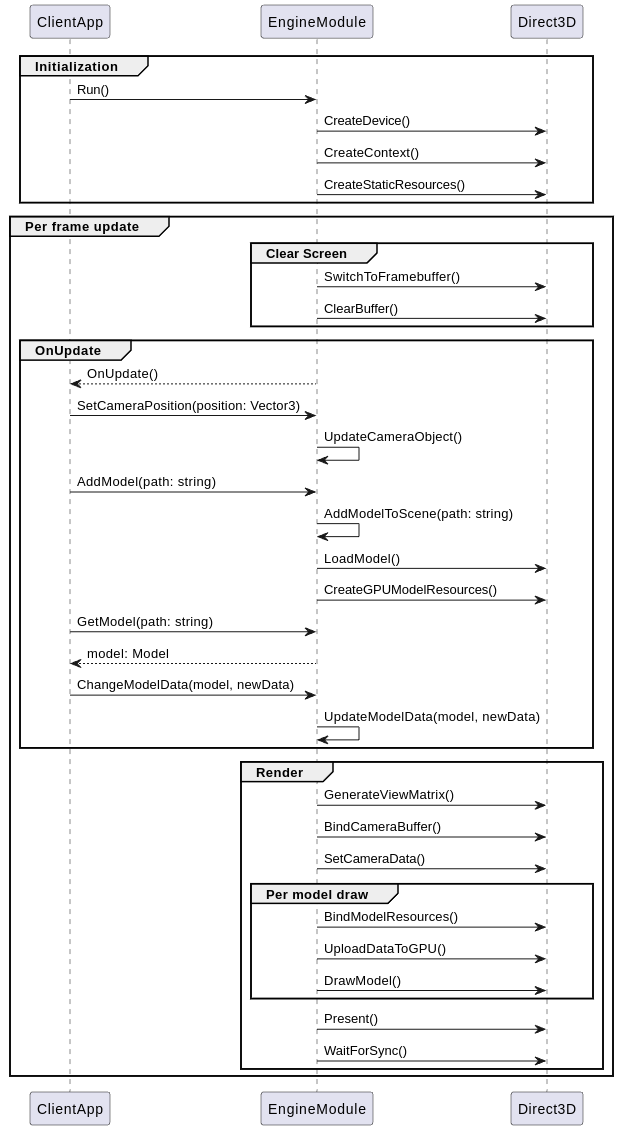
\includegraphics[width=300px]{uml/module_type_engine.png}
	\caption{Diagram przedstawiający sekwencję operowania modułu typu niezależnego z aplikacją klienta.}
	\label{UML_Sequence_Module_Engine}
\end{figure}

\vfill
\clearpage

\subsection{Abstrakcja nad API}
\label{Subsection_module_types_abstraction}
Przeciwieństwem jest moduł będący abstrakcją nad niskopoziomowymi API graficznymi. Udostępnia on uniwersalne API niezależne od systemu operacyjnego oraz końcowego API graficznego, nie zabierając przy tym kontroli nad procesem renderowania. Aplikacja klienta zarządza przepływem programu, przechowywaniem i wyświetlaniem obiektów oraz ich parametrami, a także nad dokładnym rozkładem czasowym oraz kolejnością wywoływanych metod. Ogranicza to złożoność modułu, który przejmuje na siebie utworzenie bardziej przystępnego dla programistów interfejsu.

Oczywistą wadą takiego rozwiązania jest zwiększony nakład pracy dla programisty aplikacji klienta. Ze względu na asynchroniczną charakterystykę współczesnych układów graficznych oraz ich złożoność ograniczony może zostać także potencjał wydajnościowy końcowej aplikacji. W zamian oddana jest możliwość dowolnego rozszerzania funkcjonalności modułu bez konieczności znania i modyfikacji jego kodu źródłowego.

Analogiczna do rys. \ref{UML_Sequence_Module_Engine} wizualizacja dla wersji abstrakcji została pokazana na rys. \ref{UML_Sequence_Module_Abstraction}.

\begin{figure}[ht!]
	\centering
	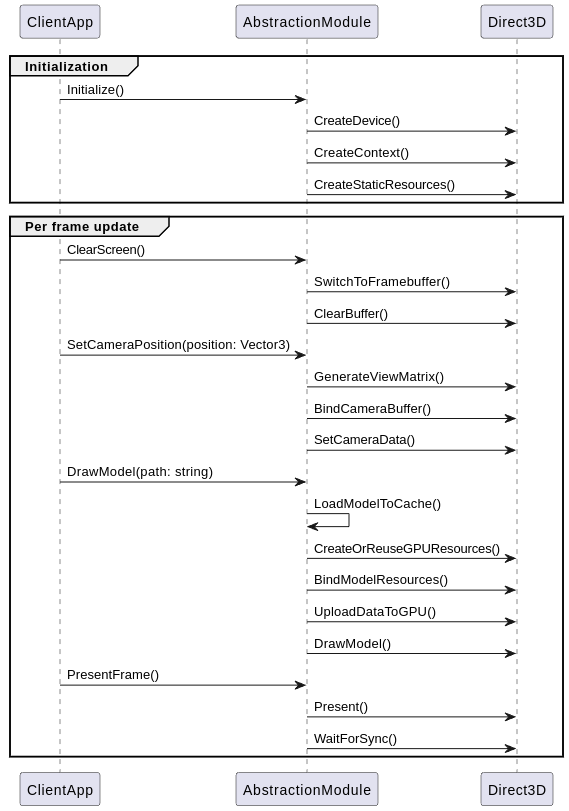
\includegraphics[width=250px]{uml/module_type_abstraction.png}
	\caption{Diagram przedstawiający sposób działania modułu abstrakcji.}
	\label{UML_Sequence_Module_Abstraction}
\end{figure}

\section{Przyjęte założenia projektowe}
Projektowany system przyjmuje formę hybrydową, korzystającą z zalet obu przedstawionych podejść do projektowania tego typu systemu. 

Głównym założeniem i podstawą implementacji zostanie utworzenie systemu warstwowego, pozwalającego na korzystanie z modułu jako abstrakcji nad API Direct3D 11 w warstwach niższych, a także na pracę w trybie niezależnym przy wyższych poziomach abstrakcji, które same będą korzystać z niższych elementów do swojego działania. Każdy z etapów umożliwiać będzie także dostęp do podległych mu komponentów. Takie podejście umożliwia mieszanie ze sobą różnych paradygmatów nie ograniczając ani potencjalnej funkcjonalności, ani przystępności dla nowych projektów i programistów.

Logistycznie projekt został podzielony na następujące warstwy:

\subsection{\textbf{Core} - Warstwa rdzeniowa}
Klasyczna warstwa abstrakcji. Grupuje często używane funkcje oraz struktury z DirectX do łatwych w użyciu elementów obiektowych, takich jak Window, Shader, Framebuffer, czy Mesh. Udostępnia funkcjonalność wczytywania z dysku plików tekstur i modeli. Do zadań tej warstwy należy też zarządzenia pamięcią oraz cyklem życia obiektów, co odbywa się automatycznie stosując inteligentne wskaźniki ze standardu C++11 oraz ComPtr z bibliotek WinAPI.

Warstwa ta udostępnia interfejs zbliżony konceptem do modułu abstrakcji z sekcji \ref{Subsection_module_types_abstraction}. 

\subsection{\textbf{Scene} - Warstwa sceny}
Na tym poziomie znajdują się wysokopoziomowe struktury oraz metody wczytywania i zarządzania sceną oraz jej komponentami. Automatyzowane jest tutaj między innymi wczytywanie z pliku pełnego modelu wraz z jego teksturami i parametrami materiałów. Segment ten odpowiada też za zachowanie wzajemnych relacji między obiektami z uwzględnieniem ich transformacji.

\subsection{\textbf{Engine} - Warstwa renderująca}
Implementacja modułu typu niezależnego. Aplikacja klienta przekazuje przy inicjalizacji parametry sceny, pozycje oraz ustawienia modeli, wirtualnej kamery i oświetlenia. Wartości te mogą być modyfikowane w przekazanej do modułu funkcji typu callback, wywoływanej automatycznie przed rysowaniem kolejnej klatki obrazu, tak jak zostało to opisane w sekcji \ref{Subsection_module_types_engine}. Możliwe jest także przełączenie w tryb ręczny zbliżony do wersji z podrozdziału \ref{Subsection_module_types_abstraction}, w którym za wywoływanie funkcji rysowania oraz synchronizację odpowiedzialna jest aplikacja klienta. Na tym poziomie obecna jest także logika ułatwiająca pracę z buforami, oświetleniem, pakiet standardowych shader'ów czy menadżer zasobów.

Interakcja między aplikacją klienta, a modułem została przedstawiona na rys. \ref{UML_Sequence_Module_Final}. W przypadku trybu ręcznego etap \textit{EngineLoop} zostaje pominięty i jego funkcjonalność przejmuje aplikacja klienta.

\begin{figure}[ht!]
	\centering
	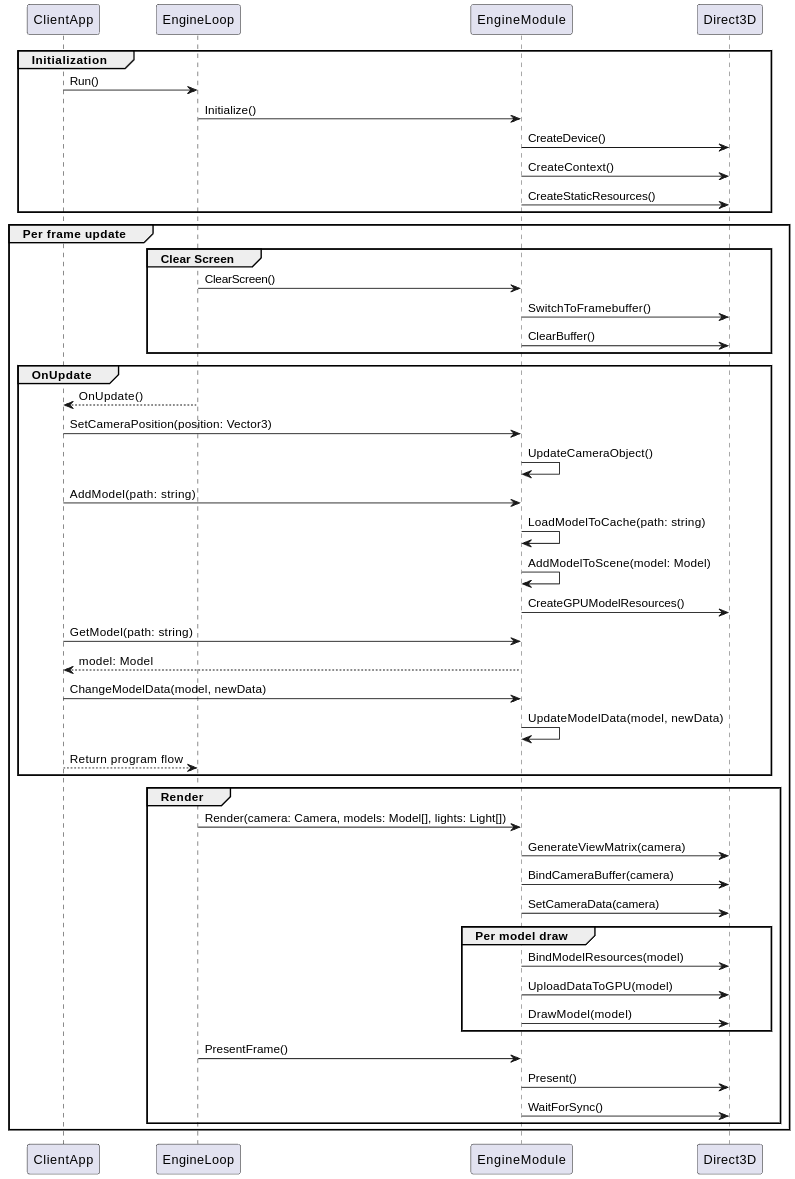
\includegraphics[width=350px]{uml/module_type_final.png}
	\caption{Diagram przedstawiający sposób działania modułu abstrakcji.}
	\label{UML_Sequence_Module_Final}
\end{figure}
    \chapter{Implementacja}
W poniższym rozdziale opisane zostały prace nad modułem, przyczyny oraz uzasadnienie poszczególnych decyzji projektowych oraz problemów, które po drodze wyniknęły. Finalna architektura wraz z pełnym wyjaśnieniem funkcjonalności poszczególnych komponentów została opisana w rozdziale \ref{chapter_System_Architecture}.

\section{Podstawowy projekt zapoznawczy}
Pierwszym krokiem w utworzeniu modułu było utworzenie aplikacji testowej. Używa ona tych samych bibliotek oraz API co końcowy moduł, ale w formie okrojonej, nie realizując założeń architektury systemu, a jedynie MVP - Minimal Viable Product. Takie rozwiązanie pozwala na zapoznanie się z praktycznym wykorzystaniem używanych później interfejsów, a także na stworzenie wzorca do pierwszej implementacji faktycznego modułu docelowego.

Prace nad aplikacją rozpoczęto od utworzenia rozwiązania w programie Visual Studio 2022 na podstawie załączonego do niego wzorca - \textit{Direct3D 11 Game Win32} \cite{GitHub:walbourn:directx-vs-templates}, zawierającego prekonfigurowany projekt wykorzystujący Direct3D oraz DirectXTK. W ramach szablonu zawarte są też podstawowe metody tworzenia zasobów używanych w ramach D3D, a także przyjęta przez jej autora struktura sterowania przepływu kodu - inna od zaplanowanej w ramach modułu. Następnie dodane zostały zgodne z założeniami biblioteki i przetestowano poprawność konfiguracji. Do tak skonfigurowanego projektu dodane zostały metody wczytywania geometrii podstawowych modeli za pomocą biblioteki assimp, a także bez określonej struktury kod odpowiedzialny za ich dodatkową obróbkę oraz finalne renderowanie. Projekt aplikacji zapoznawczej został zakończony implementacją widoku z obracającym się, kolorowym trójkątem, przedstawionym na rys. \ref{Impl_TemplateProject}.

\begin{figure}[h!]
	\centering
	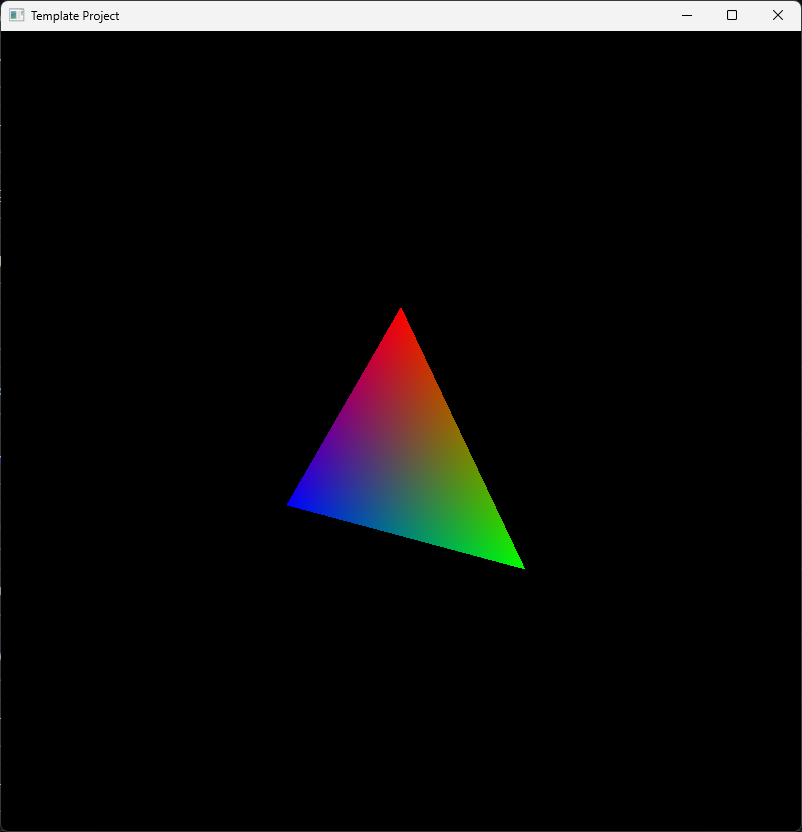
\includegraphics[width=300px]{images/impl/1_template_project.png}
	\caption{Statyczny obraz obracającego się trójkąta w ramach projektu zapoznawczego.}
	\label{Impl_TemplateProject}
\end{figure}

\vfill
\clearpage

\section{Moduł rdzeniowy}
Tak przygotowany projekt umożliwiał względnie proste utworzenie aplikacji renderującej wczytany z dysku model, ale ze względu na brak konkretnej architektury oraz celu nie nadawał się do dalszego rozwoju. Kolejnym krokiem było więc przeniesienie już istniejących funkcjonalności do formy zgodnej z docelową architekturą, możliwą do dalszego rozwoju. W tym celu utworzona została podstawowa struktura \textbf{D3DEngine} (przemianowana później na \textbf{D3DCore}), przechowująca referencje do rdzeniowych zasobów systemu Direct3D oraz okna, a także odpowiedzialna za tworzenie, odpowiednie zarządzanie, użyczanie i zwalnianie tych zasobów. W kolejnym kroku do klasy dodane zostały nadpisywalne obiekty wskaźników na funkcje zdarzeń, wywoływanych przy niektórych interakcjach użytkownika z oknem - takich jak jego przesunięcie, zmiana rozmiaru czy aktywnego okna. Poprawiona została także wydajność ze względu na przejście ze starego trybu publikacji klatek obrazu - DXGI\_SWAP\_EFFECT\_BLIT - na nowy - DXGI\_SWAP\_EFFECT\_FLIP. 

\subsection{Wiele okien - wiele problemów}
W tym momencie zapadła decyzja, według której powinna być możliwość niezależnego działania wielu instancji modułu jednocześnie, co pozwoliłoby na utworzenie aplikacji klienta z funkcjonalnością otwierania wielu okien w ramach jednej aplikacji. Z takim podejściem wiąże się natomiast problem - WinAPI posiada możliwość zdefiniowania funkcji odpowiadającej na event zdarzeń okna \textit{(WndProc)}, ale bez bezpośredniej możliwości powiązania uchwytu okna do własnej struktury go reprezentującej. Po wielu testach różnych rozwiązań ostatecznie problem został rozwiązany pewnym obejściem. Przy tworzeniu okna wskaźnik na strukturę \textit{Window} zostaje przekazany jako ostatni argument funkcji CreateWindowEx - \textit{(lpParam)}. Następnie między WinAPI, a faktycznym eventem WndProc dodany zostaje pośrednik - WndProcDispatcher. Nasłuchuje on konkretnych typów zdarzeń i jeśli otrzyma event typu \textit{WM\_NCCREATE}, oznaczający utworzenie nowego okna, pobiera wskaźnik do struktury \textit{Window} przekazany jako pole struktury \textit{LPCREATESTRUCT} w argumencie lParam. Następnie wykonuje powiązanie z uchwytem do okna przy pomocy mechanizmu \textit{SetWindowLongPtr()}. Dzięki takiemu podejściu w kolejnych wywołaniach \textit{WndProcDispatcher} możliwe jest pobranie wskaźnika do powiązanej z uchwytem struktury przy pomocy funkcji \textit{GetWindowLongPtr()}, a w związku z tym wywołanie metody \textit{WndProc} na odpowiednim oknie. Pseudokod realizujący opisany mechanizm został przedstawiony na listingu \ref{lst:module:WndProcDispatcher}.

\begin{lstlisting}[caption={Pseudokod integracji wskaźnika okna z uchwytem HWND}, label={lst:module:WndProcDispatcher}]
void Window::Create() {
 ...
 CreateWindowEx(..., this);
 ...
}

LRESULT WndProcDispatcher(HWND hwnd, UINT message, (...), LPARAM lParam) {
 if (message == WM_NCCREATE) {
     Window* win = (LPCREATESTRUCT)lParam -> lpCreateParams;
     SetWindowLongPtr(hwnd, GWLP_USERDATA, win);
 }
	
 Window* win = GetWindowLongPtr(hwnd, GWLP_USERDATA);
 return win->WndProc(...);
}
\end{lstlisting}

\subsection{Mesh i typy wierzchołków}
Kolejnym napotkanym problemem okazał się być temat typu wierzchołków w ramach modeli i mesh'y. Do poprawnego działania Direct3D wymaga określenia struktury danych wejściowych w ramach mechanizmu InputLayout, która zmienia się w zależności od użytej struktury opisującej typ wierzchołków. Oczywistym rozwiązaniem byłoby użycie mechanizmu szablonowania z języka C++, ale wymagałoby to ręcznego i zewnętrznego definiowania implementacji metody zwracającej D3DInputLayout dla każdego typu wierzchołka z osobna, co jest bardzo podatnym na błędy i nieprzejrzystym rozwiązaniem. Tutaj także udało się znaleźć lepsze rozwiązanie, którym okazał się być wprowadzony w ramach C++20 mechanizm \textit{concepts} \cite{cpp20:concepts:2025}. W ramach tego mechanizmu możliwe jest zdefiniowanie \textit{konceptu}, czyli ograniczeń dla typów szablonowych narzucających im konieczność zawarcia określonej metody. Dzięki temu utworzony został koncept \textit{VertexTypeConcept}, który wymaga utworzenia metody \textit{GetInputLayout()}, zwracającej D3DInputLayout przystosowany do pracy z danym typem.

\subsection{Lewoskrętny układ współrzędnych}
Przewijającym się przez cały proces developmentu - a w tym momencie po raz pierwszy - problemem był także przyjęty jako zalecany w ramach Direct3D lewoskrętny układ współrzędnych, w którym oś +Z rośne wraz z głębokością "w ekranie". Jest to przeciwieństwo układu prawoskrętnego z odwróconą osią Z, wykorzystywanego przez większość konkurencyjnych API, takich jak OpenGL i Vulkan. Duża część otwarto-źródłowych bibliotek oraz dostępnej dokumentacji opiera się na drugiej opcji, co skutkowało okazjonalnymi problemami z mieszaniem skrętności układów współrzędnych. Assimp posiada flagę postprocessingu, mającą na celu zmianę układu na lewoskrętny - \textit{aiProcess\_ConvertToLeftHanded} - która wydawała się pomóc na tym etapie, ale ostatecznie nie naprawiła problemu całkowicie, przez co będzie on wracać.

\vfill

\begin{figure}[h!]
	\centering
	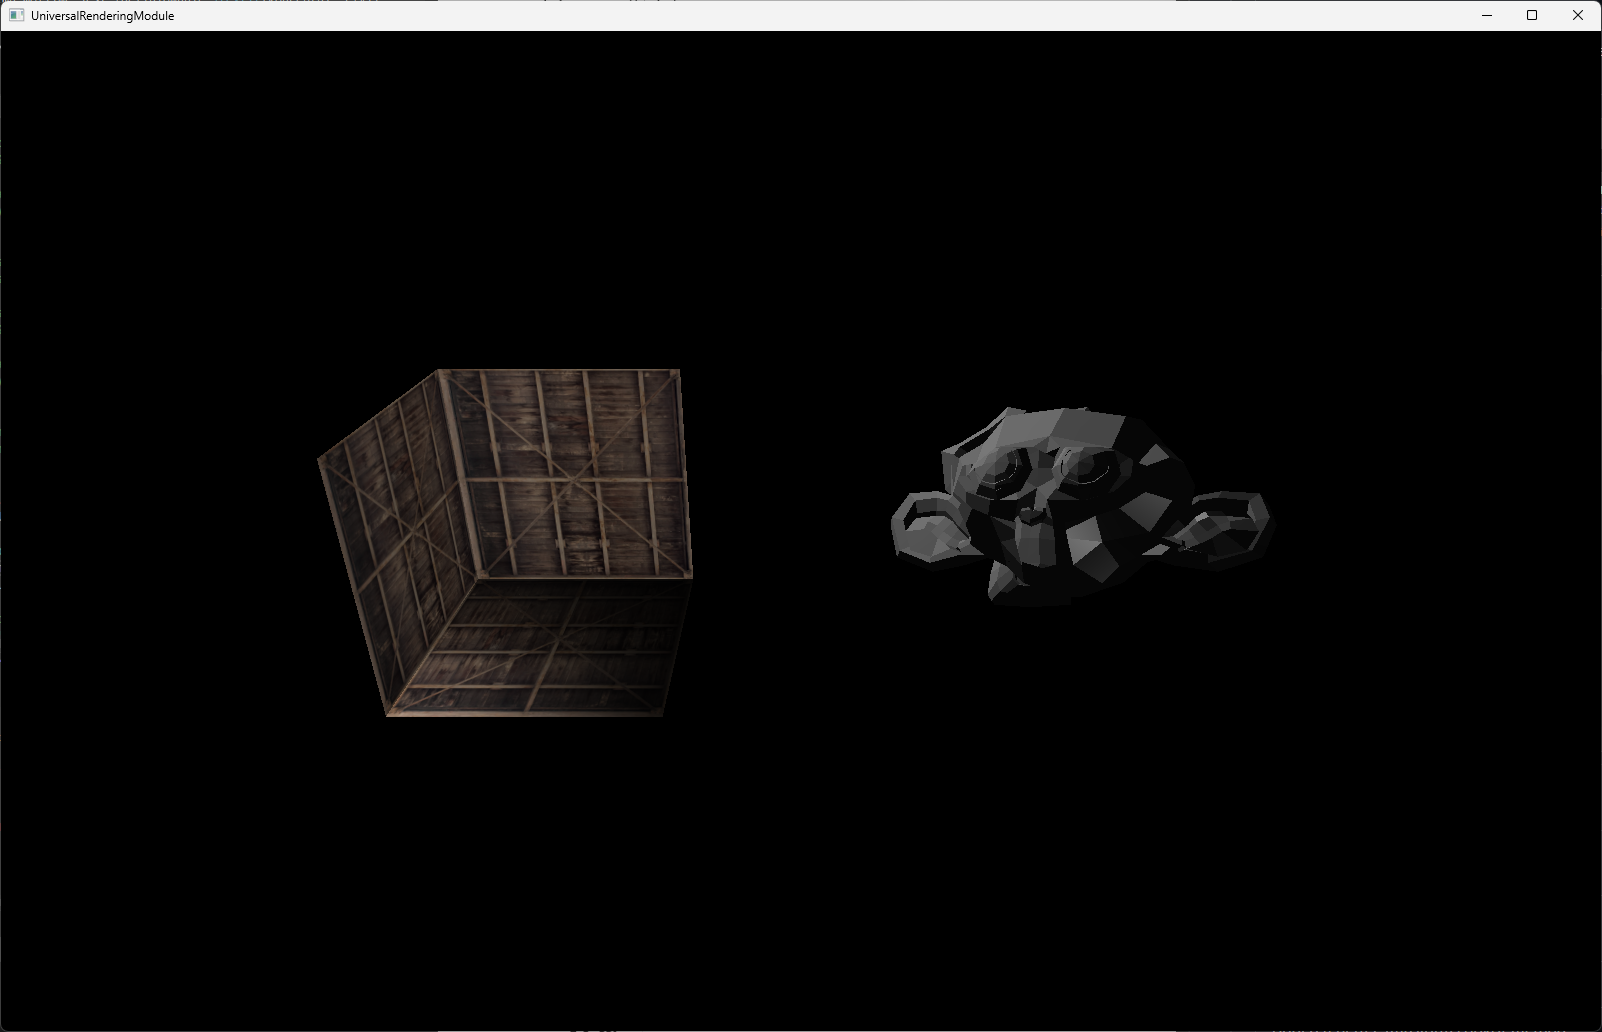
\includegraphics[width=300px]{images/impl/3_inverted_handiness.png}
	\caption{Odwrócona skrętność sortowania wielokątów z widocznym rezultatem w postaci zniekształconych modeli.}
	\label{Impl_InvertedHandiness}
\end{figure}


\subsection{Właściwości materiałów - wczytywanie}
Dane właściwości materiałów, takie jak jego kolor, chropowatość i inne parametry są odczytywane i dekodowane przez assimp przy wczytywaniu plików modeli. Dane te zapisane są jednak w formie tablicy bajtów, niezależnie od tego jaki typ reprezentują. Wczytanie takich danych wiąże się z dwoma potencjalnymi trudnościami - endianness architektury oraz brak wsparcia dla operacji na bitach przy typach zmiennoprzecinkowych.

Pierwszy problem opisuje potencjalną niekompatybilność bitowego zapisu wielobajtowych danych dla różnych architektur. W przypadku systemów Big Endian, dane przechowywane są bajtami w kolejności od najbardziej do najmniej znaczącego, gdzie Little Endian sortuje je odwrotnie. Brak konwersji między typami spowodowałby niepoprawną interpretację danych, a w rezultacie błędne parametry wynikowe. Najważniejsze architektury na rynku są jednak zgodne - procesory ARM oraz x86 operują na założeniu Little Endian \cite{ARM:Developer:Endianness} \cite{Oracle:HelpCenter:x86ByteOrdering}. W związku z tym podjęta została decyzja, aby nie dodawać osobnej ścieżki kodu dla architektur Big Endian, ze względu na niską popularność takich systemów.

Druga trudność wynika ze standardu IEEE 754, opisującego standard typów zmiennoprzecinkowych \textit{(ang. floating point)}, na podstawie którego zaimplementowany został typ float w języku C++. Standard ten zabrania bezpośredniej manipulacji bitami i konwersji bitowej z innych typów, a jedynie na konwersję wartości. Fakt ten nie pozwala na łatwe wczytanie zapisanych w formie tablicy bajtów liczb zmiennoprzecinkowych i wymaga obejścia, polegającego na konwersji wskaźnika do wskazującego typu float, a następnie pobranie jego wartości.  W taki sposób, przedstawiony na listingu \ref{lst:module:floatingPointHack}, możliwe jest wczytanie reprezentacji bitowej do formy natywnej zmiennej typu float.

\begin{lstlisting}[caption={Bitowa konwersja typu całkowitego na float w C++}, label={lst:module:floatingPointHack}]
// Wczytanie danych z tablicy bitów
int numberFromBytes = loadBytes();

// Wczytanie adresu do wskaźnika
int* nfbPointer = &numberFromBytes;

// Konwersja wskaźnika typu całkowitego na typ float
float* fprPointer = (float*)nfbPointer;

// Pobranie wartości z nowego wskaźnika.
float floatingPointRepresentation = *fprPointer;
\end{lstlisting}

\subsection{Właściwości materiałów - przechowywanie}
Po wczytaniu parametry materiału należy także przechować. Ze względu na specyfikę tych danych - a w szczególności różne typy danych zależnie od rodzaju parametru - pojawił się problem w jaki sposób powinno to zostać zrealizowane. Pierwotnie rozważane było użycie polimorfizmu ze wspólnego interfejsu, ale specyfika użycia wymagałaby każdorazowej konwersji na typ pochodny, co zmniejsza użyteczność takiego rozwiązania. W związku z tym zdecydowano się na użycie unii między typami przy pomocy mechanizmu \textit{union} oraz dodatkowej zmiennej przechowującej aktualnie przechowywany typ. Unia składała się z dynamicznie alokowanej tablicy dla wektorów typów liczbowych i std::string do tekstu. Odczyt odbywał się przy pomocy dedykowanych do tego metod, które przed zwróceniem danych sprawdzały poprawność żądania. 

Po dokładnych testach mechanizm ten nie okazał się jednak niezawodny, gdyż śledzenie stanu unii oraz odpowiedniej dealokacji i realokacji przy wszystkich przypadkach brzegowych okazało się niepraktyczne i podatne na błędy. Ze względu na to unia zastąpiona została przy pomocy obiektu typu std::variant ze standardu C++17 \cite{cpp17:variant:2025}. Jest on bezpieczniejszym zamiennikiem dla unii, posiadającym wbudowane wsparcie dla złożonych mechanizmów zarządzania obiektami i pamięcią ze standardów po C++11. Sposób odczytu danych pozostał niezmieniony.

\subsection{Odtworzenie funkcjonalności projektu zapoznawczego}
Na tym etapie przeniesione zostało już większość funkcjonalności z projektu zapoznawczego, więc możliwym było zupełne usunięcie zależności od oryginalnej klasy Game. Na koniec ponownie zaimplementowane zostało demo kręcącego się trójkąta z wykorzystaniem nowego API, co zostało przedstawione na rys. \ref{Impl_RotatingTriangle}. Symbolizuje to zakończenie prac nad warstwą rdzeniową i początek nad częścią silnika. Aby ułatwić dalszą pracę wydzielony został osobny projekt nazwany \textbf{TestApp}, pełniący funkcję aplikacji klienckiej.

Rekreacja napisana przy pomocy nowego API nie straciła na wydajności względem swojego wzorca, osiągając bardzo zbliżoną wydajność w okolicach 10.000 klatek na sekundę. Wyraźnie obniżyła się za to złożoność kodu klienckiego, którego objętość zmalała z około 1500 linijek kodu do 250. 

\begin{figure}[h!]
	\centering
	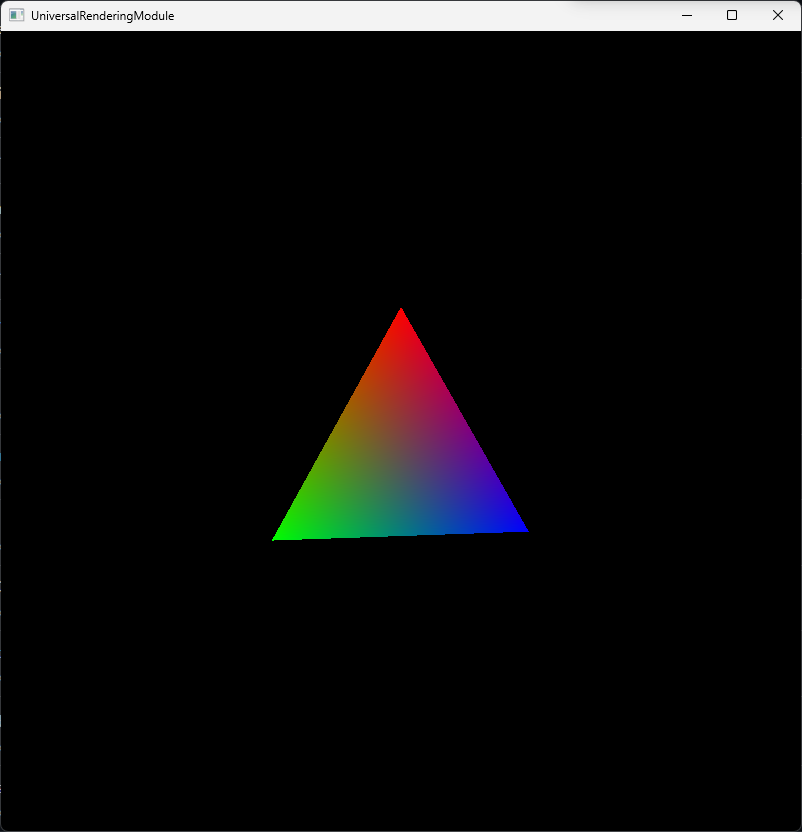
\includegraphics[width=300px]{images/impl/2_rotating_triangle.png}
	\caption{Rekreacja projektu zapoznawczego przy pomocy API modułu.}
	\label{Impl_RotatingTriangle}
\end{figure}

\vfill

\section{Warstwa sceny}
Po ukończeniu warstwy rdzeniowej przyszła kolej na część sceny. Implementacja jej funkcjonalności rozpoczęła się od utworzenia bazowego obiektu sceny oraz struktury nimi zarządzającej - \textbf{Scene}. Następnie zaimplementowane zostały metody tworzenia, usuwania oraz przypisywania do hierarchii obiektów - odpowiednio \textit{Instantiate()}, \textit{Destroy()} i \textit{SetParent()}. Wzajemna hierarchia obiektów musiała zostać podparta strukturą zarządzającą ich wzajemnymi relacjami oraz transformacjami przestrzennymi, w związku z czym powstała odpowiedzialna za to klasa \textbf{Transform}, wykorzystująca macierze transformacji do odwzorowania wzajemnych relacji między obiektami.

\subsection{Gimbal Lock}
Jednym z częściej spotykanych problemów w reprezentacji transformacji jest rotacja. Jej intuicyjna implementacja w postaci wektora trzech elementów reprezentujących rotację w 3 osiach przestrzeni jest bowiem podatna na błąd zwany \textit{Gimbal Lock}. Jest to sytuacja, w której wraz z obrotem obiektu obraca się także układ współrzędnych wokół którego jest on obracany, a w rezultacie wykonanie tych samych rotacji w innej kolejności może doprowadzić do innej pozycji wynikowej, co zostało pokazane na rys. \ref{GimbalLock}.

Rozwiązaniem jest dodanie czwartego wymiaru o aktywnym balansie, określającego "niezależny" układ współrzędnych. Standardem realizacji tego konceptu jest struktura kwaternionów, która po dodaniu metod balansujących idealnie nadaje się do reprezentacji rotacji w przestrzeni trójwymiarowej. Do dalszej pracy użyta została implementacja \textit{Quaternion} zawarta w ramach pakietu SimpleMath.

\vfill

\begin{figure}[h!]
	\centering
	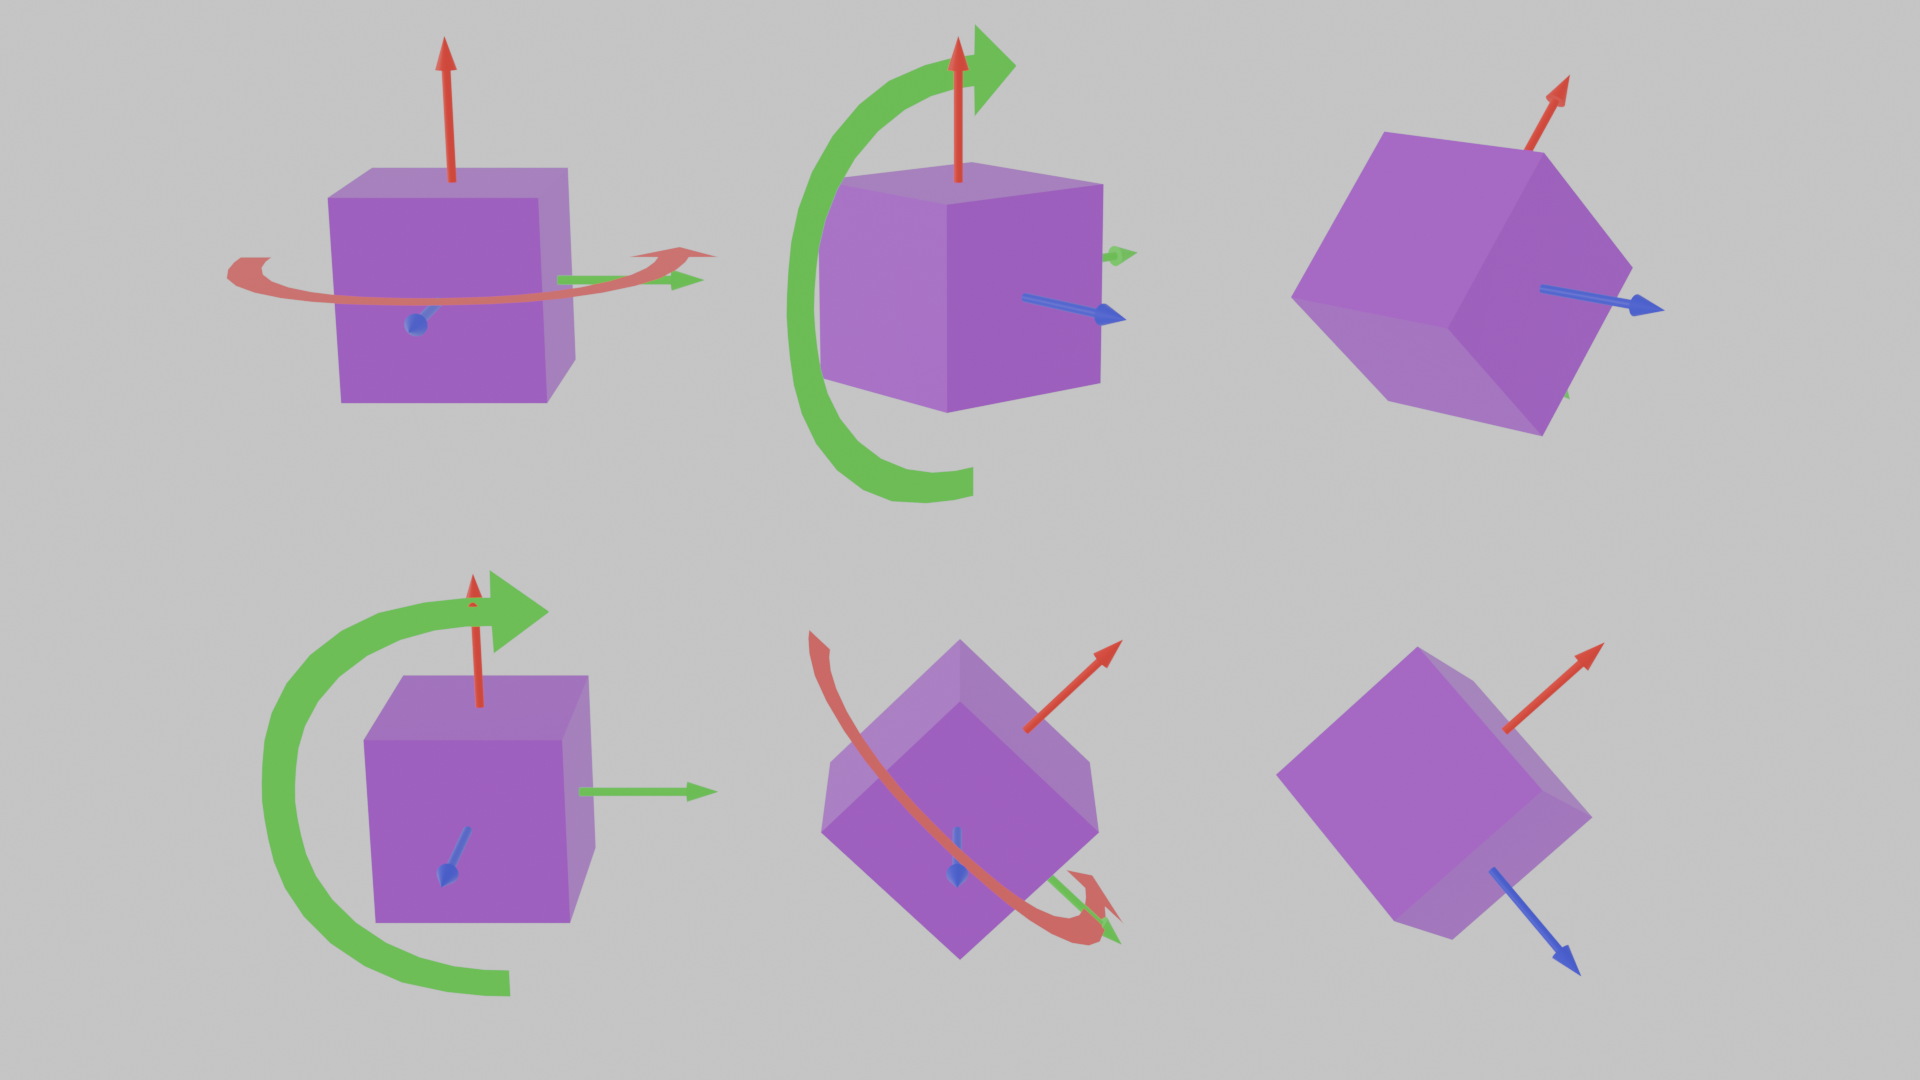
\includegraphics[width=\textwidth]{images/gimbal_lock.png}
	\caption{Wizualizacja efektu gimbal lock.}
	\label{GimbalLock}
\end{figure}

\subsection{Transformacje w przestrzeni}
Autor miał już doświadczenie w projektowaniu komponentów zbliżonych do \textit{Transform}, ale opierało się ono na API OpenGL i bibliotece GLM, zamiast użytego w projekcie Direct3D i DirectXTK / SimpleMath. Większość metod udało się utworzyć z małymi zmianami, ale problemem okazała się być metoda \textit{LookAt(target, upVector)}, która obraca obiekt w stronę przekazanej w ramach parametru \textit{target} docelowej pozycji w przestrzeni. Pakiet GLM zawiera dedykowaną do tego funkcja glm::lookAt() \cite{glm:docs:look_at}, której odpowiednika brakuje w pakiecie DirectXTK, więc funkcjonalność musiała zostać odtworzona. 

Pierwszym podejściem była próba wykorzystania dostępnej w DXTK metody \textit{XMMatrixLookAtLH()}, tworzącej macierz transformacji odpowiadającą rotacji kamery patrzącej na odpowiedni punkt. Wynikową strukturę należy następnie odwrócić, aby przekonwertować ją na wersję dla obiektu i na jej podstawie utworzyć kwaternion rotacji. 

\subsection{Problemy z wydajnością konstruktorów kopiujących}
W trakcie tworzenia modułu okazjonalnie sprawdzana była jego wydajność, która przez większość czasu wahała się w okolicach 10.000 FPS \textit{(ang. Frames Per Second)}. Była to przyjęta granica wynikająca z limitów innych niż wydajność samego modułu, gdyż minimalna aplikacja testowa składająca się jedynie z logiki czyszczenia i prezentowania klatek obrazu nie przekraczała tego poziomu wydajności. 

W okolicach tego punktu zauważony został jednak nagły spadek do poziomu około 2.000 FPS, mimo użycia sceny identycznej do pierwotnej - obracającego się trójkąta. Po analizie problemem okazało się przekazywanie wielu struktur, takich jak lista wierzchołków, w formie kopiującej zamiast referencji. Zmiana problematycznych wystąpień naprawiła problem, ale nie gwarantowała, że nie wróci on w przyszłości. Standard C++ od wersji 11 zawiera słowo kluczowe \textbf{auto}, które automatycznie określa typ zmiennej na podstawie przypisanej do niej wartości. Mechanizm ten nie obejmuje detekcji referencji i wskaźników, co spada na ręce programistów, nie pokazując przy tym żadnego błędu ani ostrzeżenia w przypadku użycia konstruktora kopiującego zamiast referencyjnego, a czego przykład został pokazany na listingu \ref{lst:module:cppcopyingref}. W związku z tym aby zapobiec przypadkowemu użyciu spowalniającej działanie programu metody kopiującej wprowadzona została pomocnicza klasa \textbf{NonCopyable}, która wyłącza konstruktory kopiujące w każdej klasie z niej dziedziczącej, pozostawiając przy tym dostępny mechanizm przenoszenia przy pomocy \textit{std::move}. W ten sposób oznaczone zostały najważniejsze klasy, takie jak \textit{D3DCore}, \textit{Window}, \textit{Scene}, a później także \textit{Engine}. 

\begin{lstlisting}[caption={Przykład sytuacji, w której łatwym jest użycie formy kopiującej zamiast referencji, co skutkuje dużym kosztem wydajnościowym.}, label={lst:module:cppcopyingref}]
	
class Data {
    int field = 5;
};

class DataHolder {
    Data data;
	
public:
    Data& GetData() {
        return data;
    }
};

int main() {
    DataHolder holder;
	
    // Wywołanie konstruktora kopiującego
    auto data = holder.GetData();
	
    // Poprawna forma referencyjna
    auto& dataRef = holder.GetData();
}
	
\end{lstlisting}

\subsection{Podsumowanie modułu sceny}
Warstwa scenowa nie przyniosła wyraźnych zysków ani spadku wydajności, a także nie uprościła znacząco kodu klienckiego w przypadku testowego programu z trójkątem. Pozwoliła ona jednak na łatwą obsługę znacznie większych objętościowo światów, a także postawiła podwaliny pod kolejny submoduł - warstwę silnika.

\section{Moduł silnika}
Prace nad warstwą rozpoczęto od wydzielenia nowego projektu i utworzenia odpowiedniej klasy - \textbf{Engine}, mającej przejąć większość obowiązków związanych z rysowaniem modeli, zarządzaniem sceną i stanem związanym z obiektami niższych warstw zarządzającymi komunikacją z API Direct3D. Początkowo zaimplementowane funkcjonalności były jedynie przeniesieniem już istniejących funkcji z \textit{TestApp}, ale z czasem dzięki ustrukturyzowanej budowie modułu możliwe było dodanie nowych, bardziej złożonych funkcjonalności. 

\subsection{Niestandardowe programy cieniujące}
Pierwszą taką funkcjonalnością było dodanie obsługi niestandardowych shader'ów. Aby było to możliwe musiał jednak najpierw powstać ustalony schemat danych do nich oraz między nimi przesyłanych. W tym celu utworzone zostały współdzielone pliki kodu HLSL - \textbf{PixelShaderCommonTypes.hlsl} oraz \textbf{PixelShaderCommon.hlsl} - zawierających odpowiednio podstawową strukturę przesyłaną między Vertex i Pixel shader'ami oraz współdzielone struktury drugiego z nich, takie jak \textbf{Light} dla świateł i funkcja \textbf{CalculateLighting} obliczająca na ich podstawie prosty model oświetlenia. W późniejszej części dodane zostały w tym miejscu struktury opisujące dodatkowe parametry renderowanych obiektów, takie jak właściwości materiału czy oświetlenie typu PBR.

\subsection{Konflikt wydajność, a modularność}
Prawie każda decyzja projektowa poza oczywistymi zaletami ciągnie za sobą także wady. W przypadku tematu modularności częstym problemem jest ograniczony potencjał optymalizacyjny, ze względu na konieczność zachowania odpowiedniej struktury oraz brak możliwości wysokopoziomowej optymalizacji międzymodułowej. Autor zdawał sobie sprawę z tego kompromisu projektując opisywany system i stawiając przede wszystkim na modularność kosztem wydajności, ale w momencie integracji sceny z silnikiem doszło do bariery, która wymagała kompromisu na tym polu. 

Problemem okazało się przechowywanie obiektów typu cache w ramach struktury sceny, pozwalających na ograniczenie konieczności każdorazowego jej przechodzenia w celu znalezienia obiektów konkretnego, często używanego typu. Pierwszym takim przykładem była lista aktywnych w scenie modeli oraz świateł, która jest krytyczna do przyspieszenia procesu renderowania, gdyż każdorazowe przechodzenie sceny w ich poszukiwaniu przy każdym rozpoczęciu procesu rysowania wiązałoby się z dużym i stałym narzutem obliczeniowym. Problemem okazało się jednak gdzie taką listę umieścić. Intuicyjną myślą było dodanie takiego elementu do Sceny, ale nie było to możliwe, gdyż przez jej niezależność obiekt opisujący model lub światło w scenie z założenia nie mógł znajdować się w ramach tej samej warstwy, a dopiero na wyższym poziomie silnika. Takie ułożenie kłóciło się jednak z wcześniejszym założeniem, w którym niższa warstwa nie może odnosić się do obiektów z warstwy wyższej. Podobny problem byłby także gdyby umieścić listę w klasie \textit{Engine}, a dokładnie wymagałby on referencji do silnika w ramach struktury \textit{SceneObject}, będącej opisem obiektu sceny i znajdującej się na jej warstwie, co oznaczałoby konieczność odniesienia się do wyższego poziomu. 

Pierwszym testowym rozwiązaniem było dodanie do sceny wskaźnika pustego typu \textit{void*}, do którego przypisywana byłaby z wyższej warstwy struktura przechowująca potrzebne do działania dane. Problem pojawił się jednak w momencie zwalniania pamięci takiego obiektu, gdyż przez brak określonego typu nie było możliwe automatyczne wywoływanie destruktora takiej klasy, w efekcie czego pojawić się mogły wycieki pamięci. Rozwiązaniem byłoby dodanie kolejnego parametru w postaci wskaźnika funkcji destruktora, ale w połączeniu z już problematycznym interfejsem pobierania takiej struktury - brak gwarancji, że dane będą typu oczekiwanego przez warstwę klienta - podjęta została decyzja o odrzuceniu tej wersji naprawy problemu. 

Drugą wersją byłoby utworzenie interfejsu typu \textit{IScene}, z którego następnie tworzone byłyby implementacje zawierające potrzebne dane. Niestety takie podejście także cierpi na konieczność walidacji typu danych przez obiekty sceny i ich pobierania przy pomocy niebezpiecznych konwersji, w związku z czym ta opcja i jej podobne także zostały odrzucone. 

Ostatecznie przyjętym rozwiązaniem był kompromis na płaszczyźnie modularności. Warstwa rdzeniowa pozostała zupełnie niezależnym od pozostałych tworem, ale poziomy sceny i silnika zostały zintegrowane do jednej, wspólnej warstwy. Struktury cache umieszczono w ramach klasy \textit{Scene}. Takie podejście narzuca jednak problem z rozszerzalnością nowego, zunifikowanego modułu, gdyż nie ma bezpośredniej możliwości rozszerzenia jej o dodatkowe cache'owane dane. W związku z tym podjęta została decyzja o zmianie formy dystrybucji biblioteki na open-source. W większości docelowych przypadków użycia modułu nie będzie konieczności modyfikacji danych przechowywanych w ramach sceny i w takich przypadkach możliwe jest korzystanie z niego w formie prekompilowanej biblioteki, ale jeśli taka konieczność nastąpi to możliwe i zalecane jest dodanie warstwy silnika (z uwzględnioną w niej funkcjonalnością sceny) jako biblioteki w formie zintegrowanego do aplikacji klienta, modyfikowalnego kodu źródłowego. 

\subsection{DPI awareness}
Drobnym, ale istotnym problemem okazało się zachowanie aplikacji w przypadku konfiguracji komputerowych, w których skalowanie ekranu ustawione jest na wartość inną niż 100\%. System Windows raportuje w takich przypadkach rozdzielczość ekranu pomniejszoną o współczynnik skali, a następnie skaluje okna aplikacji o jej wartość. Dla przykładu przy skalowaniu 200\% i rozdzielczości monitora 4000x2000, system raportuje do aplikacji wartość 2000x1000, a następnie dwukrotnie skaluje jej okno, czego efektem jest rozmyty, niewyraźny obraz, co w wyolbrzymionej formie pokazane zostało na rys. \ref{Impl_DpiAwareness}.

Rozwiązaniem jest załączenie do modułu tzw. manifest'u, czyli informacji o obsługiwanych przez aplikację funkcjach i uwzględnienie wśród nich DPI Awareness. Aplikacja raportująca wsparcie tego rozszerzenia nie jest traktowana przez system w opisany sposób, a zamiast tego otrzymuje prawdziwe informacje o monitorze i nie jest ona skalowana. W przypadku aplikacji renderujących trójwymiarową grafikę jest to preferowany sposób działania i w związku z tym manifest został dodany do modułu. 

\begin{figure}[h!]
	\centering
	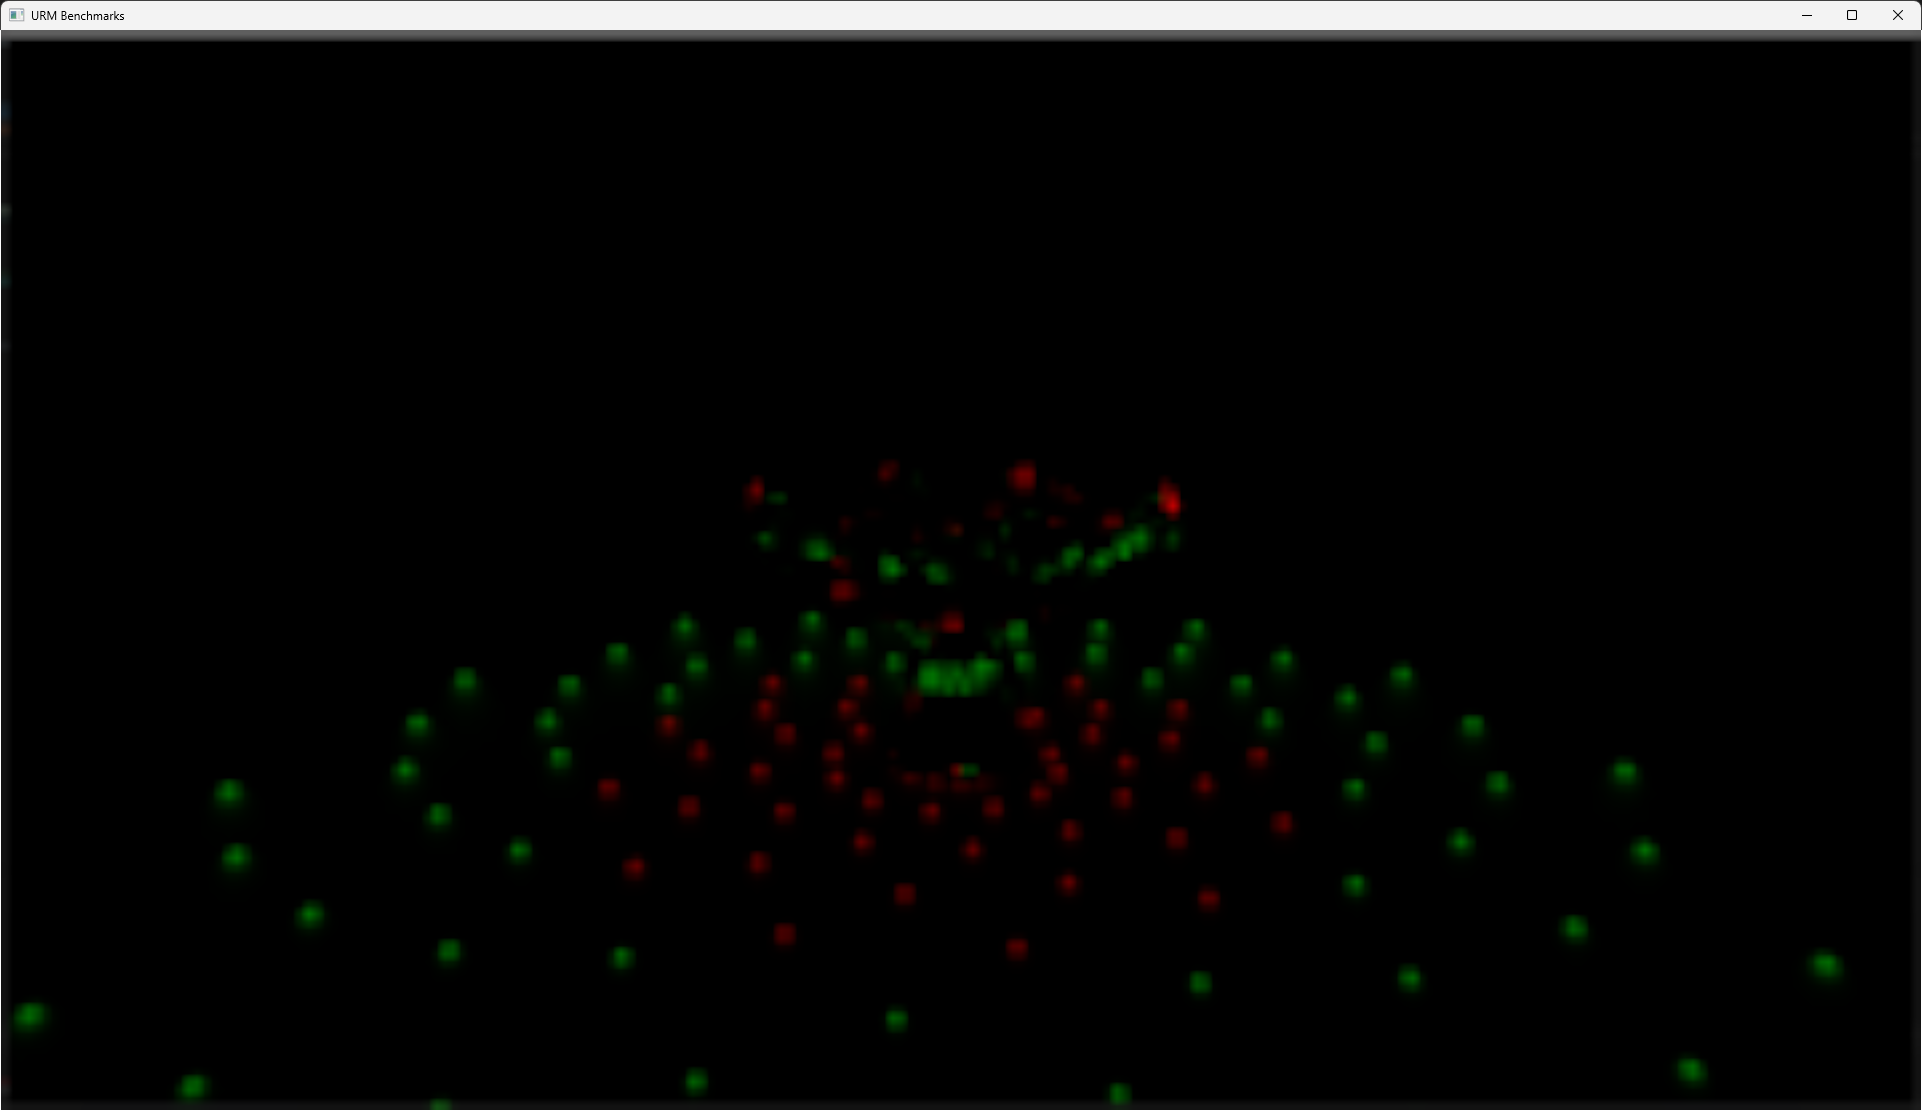
\includegraphics[width=\textwidth]{images/impl/4_dpi_awareness_8x.png}
	\caption{Wizualizacja efektu rozmycia przy braku DPI awareness aplikacji - na przykładzie dla skalowania 800\%.}
	\label{Impl_DpiAwareness}
\end{figure}

\vfill

\subsection{Caching wczytywanych modeli}
Dekodowanie danych o modelach oraz ich wczytywanie z dysku jest zadaniem wymagającym pod względem wymaganej mocy obliczeniowej i czasu potrzebnego do przetworzenia takich danych. Często spotykanym w świecie trójwymiarowych scen jest też zachowanie aplikacji, w których wczytują one pojedynczy model do wielokrotnego wykorzystania - na przykład krzak w grze z otwartym światem. Przy takim zachowaniu marnotrawnym byłoby każdorazowe przechodzenie przez proces wczytywania i dekodowania danych o tym samym modelu z dysku, więc w ramach modułu silnika utworzony został mechanizm zarządzania zasobami w postaci klasy \textbf{AssetManager}. Przechowuje ona wczytane modele i tekstury do późniejszego wykorzystania, ale pozwala także na ich zwolnienie przy zmianie sceny albo w sytuacjach o zmniejszonej dostępności wolnej pamięci podręcznej. 

\subsection{PBR i system materiałów}
Renderowanie oparte o PBR \textit{(ang. Physically Based Rendering)} jest aktualnym standardem w branży grafiki trójwymiarowej, więc obsługa renderowania o ten standard opartego została dodana do warstwy silnika. Z założenia modularności wynika jednak, że nie powinien być to jedyny wspierany system oświetlenia. Pierwszą próbą połączenia różnych typów kalkulacji świateł było wydzielenie najważniejszych komponentów Pixel Shader'a do osobnego pliku i dalszego wykorzystania. Chcąc utworzyć funkcjonalność jak najbardziej otwartą koniecznym było jednak zadbanie o nieograniczanie aplikacji klienta w kwestii tworzenia nowych, dowolnie skonstruowanych i rozwiniętych materiałów. W związku z tym wprowadzony został rozwinięty względem warstwy rdzeniowej system materiałów. Opiera się on na bazowej klasie \textbf{Material}, definiującej użyty do materiału Pixel Shader oraz przesyłanego do niego dane w postaci struktury typu \textbf{ConstantBuffer} i pozwala na zaimplementowanie wirtualnie dowolnej kombinacji materiału i programu cieniującego. 

Największym problemem związanym z takim systemem okazało się jego połączenie z autodetekcją materiałów wczytywanych modeli. Została tutaj podjęta decyzja o ograniczeniu wsparcia tego mechanizmu jedynie do oświetlenia typu PBR, ale pozostawienie możliwości ręcznej implementacji podobnej funkcjonalności na podstawie opisanych przy okazji warstwy rdzeniowej \textit{MaterialProperties}. 
    \chapter{Implementacja systemu}
	Ostateczna forma projektu przedstawiona została przy pomocy diagramów UML, wygenerowanych autorskim skryptem na podstawie kodu źródłowego gotowego programu.

\section{Warstwa rdzeniowa}
	W warstwie rdzeniowej ujęte zostały najczęściej używane struktury z pakietu Direct3D 11. Wrappery takich obiektów zostały oznaczone prefixem D3D. Pozostałe klasy posiadają nazwę bez przedrostków.

\subsection{Core}
	Klasa będąca podstawą funkcjonowania całego modułu. 
	Odpowiada za tworzenie oraz zarządzanie podstawowych zasobów używanych przez aplikacje oparte o Direct3D, takich jak Device, Context, RenderTarget(View), Swap Chain czy Framebuffer. Przy jego pomocy możliwy jest wybór trybu rysowania z listy reprezentowanej przez enum PrimitiveTopologies.
	Moduł zawiera także przez kompozycję odniesienie do obiektu klasy \textbf{Window}, która zawiera w sobie logikę odpowiedzialną za zarządzanie uchwytem do systemowego okna (i zasobami z tym związanymi) oraz odpowiedziami na zmianę jego stanu i rozmiaru.
	Inicjalizacja obu elementów odbywa się przez przekazanie w konstruktorze obiektu \textbf{WindowCreationParams}, zawierającego podstawowe informacje o tworzonym oknie.
	Diagram UML przedstawiony został na rys. \ref{UML_D3DCore}.
	
	
	\begin{figure}[ht!]
		\centering
		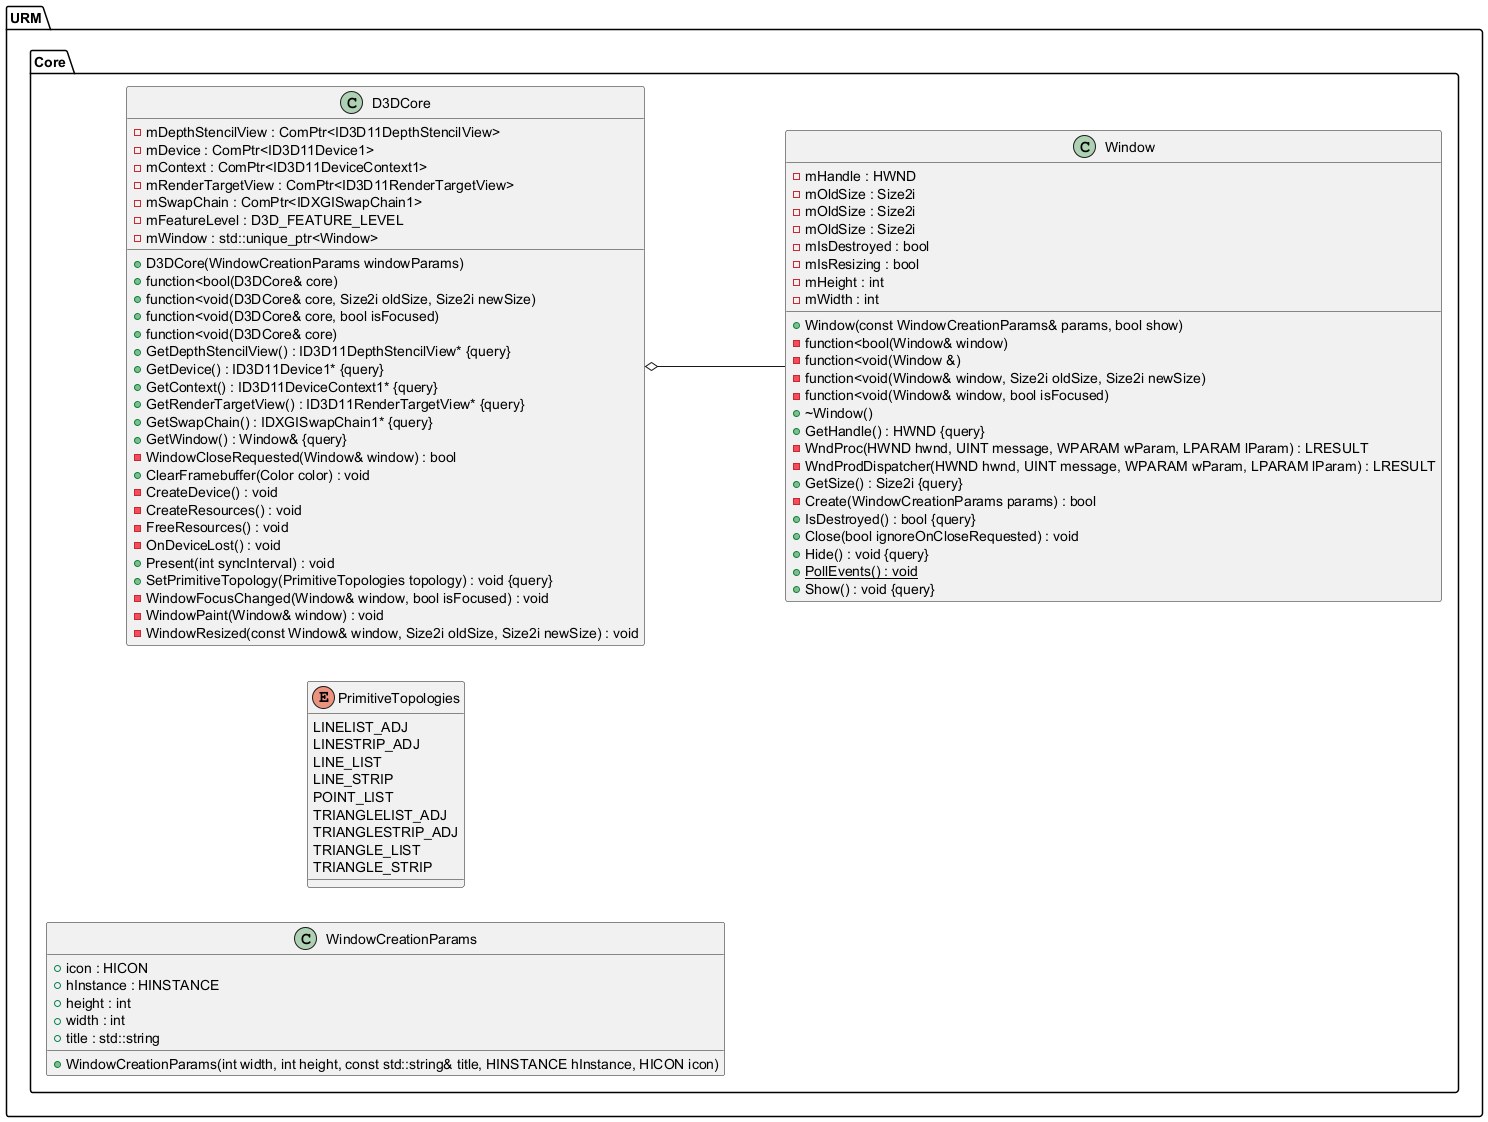
\includegraphics[width=\textwidth]{images/UML/core.png}
		\caption{Diagram UML przedstawiający kompozycję modułów D3DCore oraz Window wraz z zależnościami.}
		\label{UML_D3DCore}
	\end{figure}
	
	\vfill
	\clearpage
	
\subsection{Dziennik (Log)}
	Do prowadzenia dziennika \textit{(logu)} aktywności wykorzystana została otwartoźródłowa biblioteka \textbf{spdlog} na otwartej licencji MIT \cite{github:spdlog:spdlog}. Dodatkowo do modułu dołączona została statyczna klasa Logger opisana na rys. \ref{UML_Logger}. Udostępnia ona funkcje konfigurujące spdlog pod potrzeby projektu oraz metodę zwracającą referencję do dziennika zdarzeń krytycznych.
	

	\begin{figure}[h!]
		\centering
		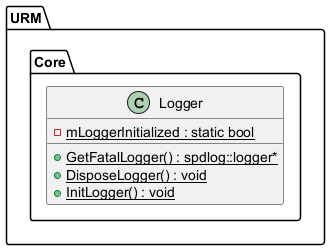
\includegraphics[width=\textwidth]{images/UML/logging.png}
		\caption{Schemat pomocniczej klasa statycznej dziennika.}
		\label{UML_Logger}
	\end{figure}
	
	\vfill
	\clearpage
	
\subsection{Metody pomocnicze}
	Sekcja zawierająca klasy i struktury pomocnicze wykorzystywane w ramach modułów projektu, przedstawione na rys. \ref{UML_Utils}.
	
	W ramach tego segmentu zaimplementowane zostały następujące klasy:
	\begin{itemize}
		\item \textbf{Size2i}: Prosta struktura opisująca rozmiar w przestrzeni 2D. Używana na przykład do określania wielkości okna.
		\item \textbf{TypeUtils}: Funkcje pomocnicze pobierania informacji o typach. Wykorzystywana między innymi do porównywania typów na podstawie wywołań generycznych.
		\item \textbf{StringUtils}: Odpowiedzialna za operacje tekstowe. Udostępnia funkcjonalność konwersji między zmiennymi tekstowymi jednobajtowymi \textit{(std::string)} oraz dwubajtowymi \textit{(std::wstring)}, a także pobierania nazwy folderu ze ścieżki do pliku.
		\item \textbf{FloatUtils}: Funkcjonalność ułatwiająca pracę z liczbami zmiennoprzecinkowymi. Dzięki metodom zawartym w tej klasie możliwe jest zbliżone porównywanie dwóch liczb typu float oraz określanie znaku tego typu liczb.
		\item \textbf{TimeUtils}: Wykorzystywana do testowania wydajności kodu. Pozwala na wywołanie dowolnej funkcji mierząc przy tym jej czas wykonania.
	\end{itemize}
	
	\begin{figure}[h!]
		\centering
		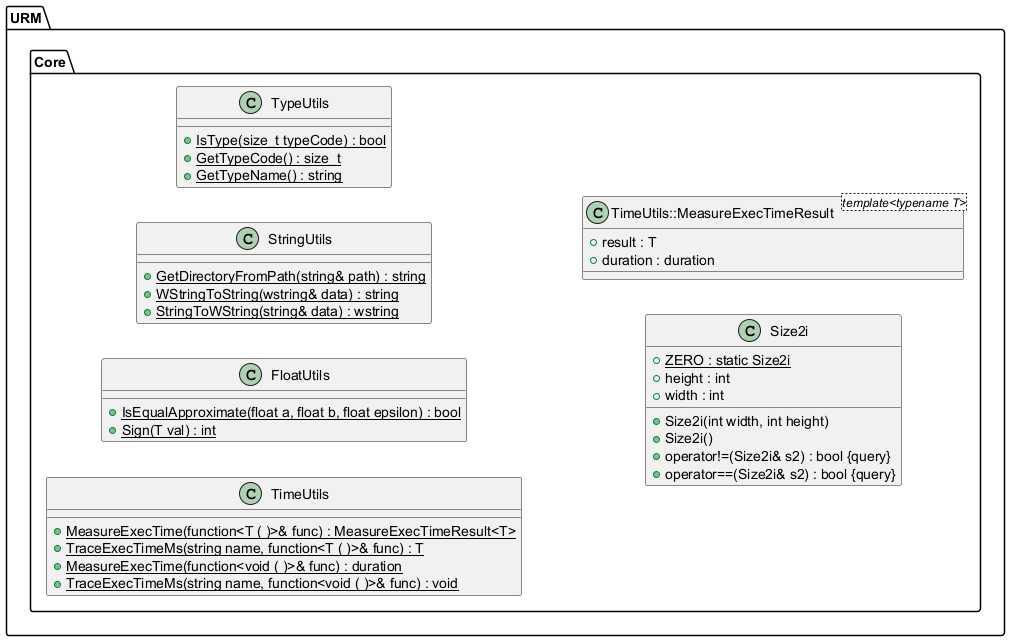
\includegraphics[width=\textwidth]{images/UML/utils.png}
		\caption{Schemat klas pomocniczych.}
		\label{UML_Utils}
	\end{figure}
	
	Do testów wydajności w trakcie oraz po zakończeniu prac nad modułem utworzona została także klasa \textbf{Stopwatch}, udostępniająca zaawansowaną funkcjonalność mierzenia czasu, a jej schemat został przedstawiony na rys. \ref{UML_Stopwatch}.
	
	\begin{figure}[h!]
		\centering
		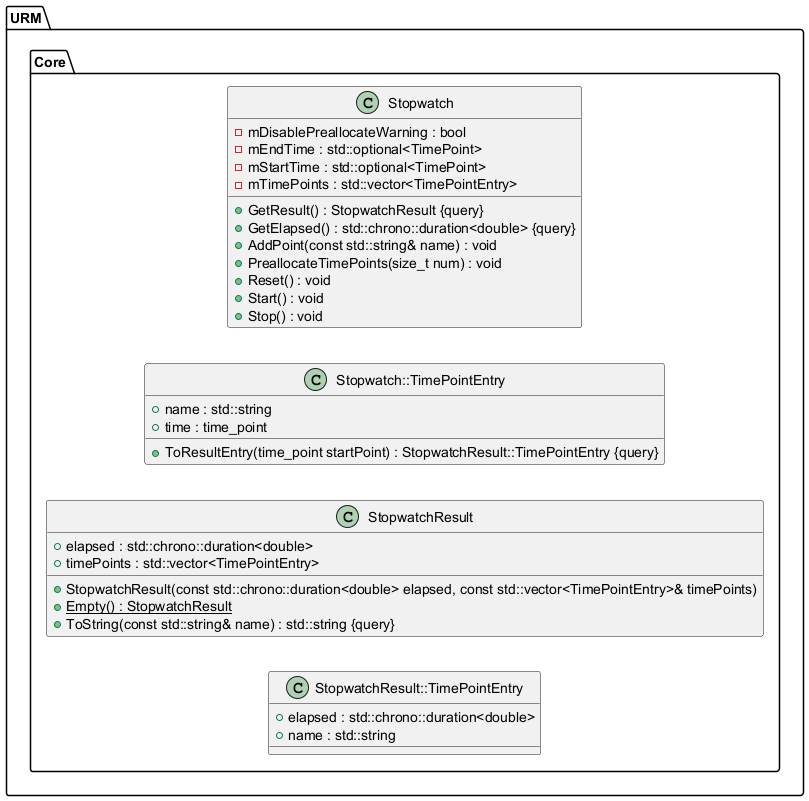
\includegraphics[width=\textwidth]{images/UML/stopwatch.png}
		\caption{Schemat klasy czasomierza.}
		\label{UML_Stopwatch}
	\end{figure}
	
\subsection{Baza D3D}
	Zbiór elementów będących warstwą abstrakcji nad niskopoziomowymi elementami pakietu Direct3D, wymaganych do jego użycia.
	\textbf{D3DViewport} odpowiedzialny jest za określanie wymiarów okna widoku (Viewport), jak i zakresu głębi rysowanego obrazu.
	Z kolei \textbf{D3DRasterizerState} pozwala na konfigurowanie parametrów procesu rasteryzacji, takich jak Culling Mode (definiowany przez enum CullModes) służący do pomijania wielokątów obróconych w złą stronę, tryb wypełnienia (przy pomocy enum FillModes), antyaliasingu, itp.
	Diagram przedstawiający strukturę opisywanych klas można zobaczyć na rys. \ref{UML_D3DUtils}
	
	\begin{figure}[h!]
		\centering
		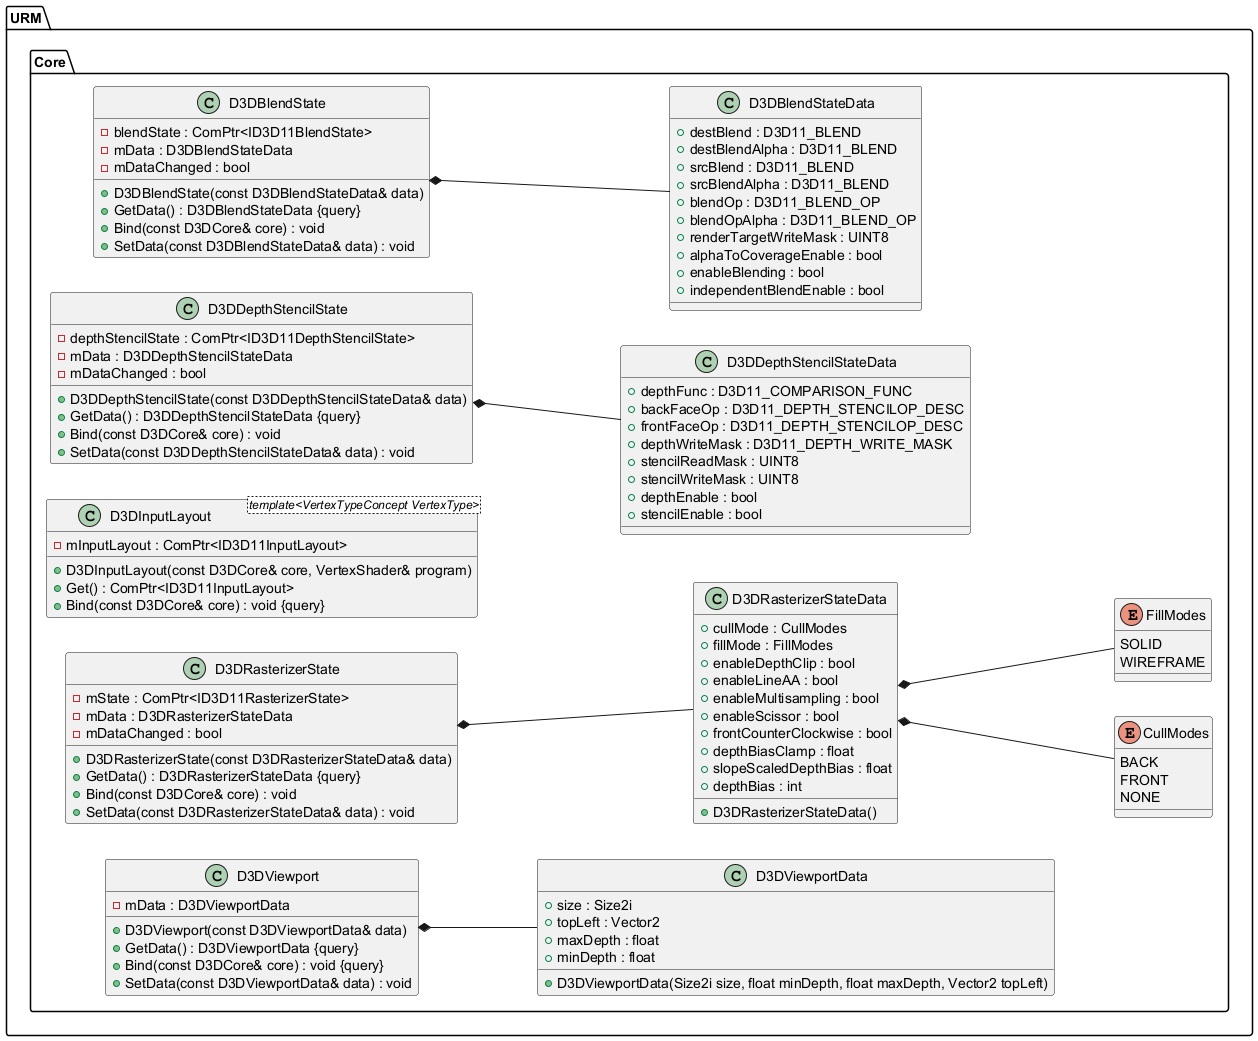
\includegraphics[width=\textwidth]{images/UML/d3dutils.png}
		\caption{Kompozycja wrapperów modułów bazowych D3D.}
		\label{UML_D3DUtils}
	\end{figure}
	
	\vfill
	\clearpage
	
\subsection{Bufory}
	Kolejnym elementem koniecznym do poprawnego korzystania z API D3D są bufory, używane jako środek przesyłu danych 
	Do ich łatwiejszej obsługi utworzona została klasa abstrakcyjna \textbf{ID3DBuffer}, której implementacje, \textbf{D3DVertexBuffer}, \textbf{D3DIndexBuffer} oraz \textbf{D3DConstantBuffer} stanowią rozwiązania do wykorzystania odpowiednio buforów wierzchołków, indeksów oraz stałych, a ich kompozycja została pokazana na rys. \ref{UML_Buffer}
	
		
	\begin{figure}[h!]
		\centering
		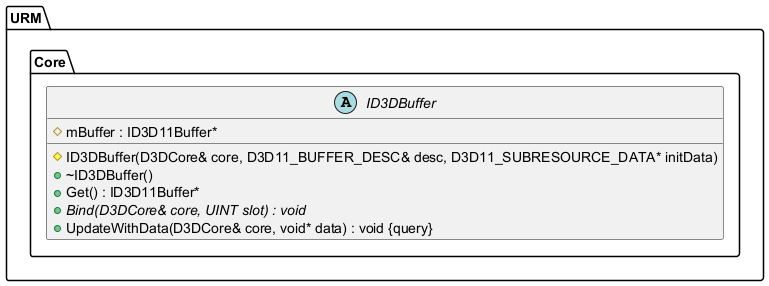
\includegraphics[width=\textwidth]{images/UML/buffer.png}
		\caption{Klasa ID3DBuffer oraz jej implementacje.}
		\label{UML_Buffer}
	\end{figure}
	
\subsection{Mesh i typy wierzchołków}
	Zbiór połączonych wielokątów wraz z opisującymi go metadanymi nazywany jest Mesh'em, którego schemat przedstawiony został na rys. \ref{UML_Mesh}.
	
	Zgodnie z założeniami projektu i ten element został zaprojektowany w modularnej formie. Wykorzystując szablon typów pozwala na pracę z różnymi typami wierzchołków. Kilka typów standardowych zostało zaimplementowanych w ramach modułu \textbf{StandardVertexTypes}, opisanego na diagramie \ref{UML_VertexTypes}.
	
	\begin{figure}[h!]
		\centering
		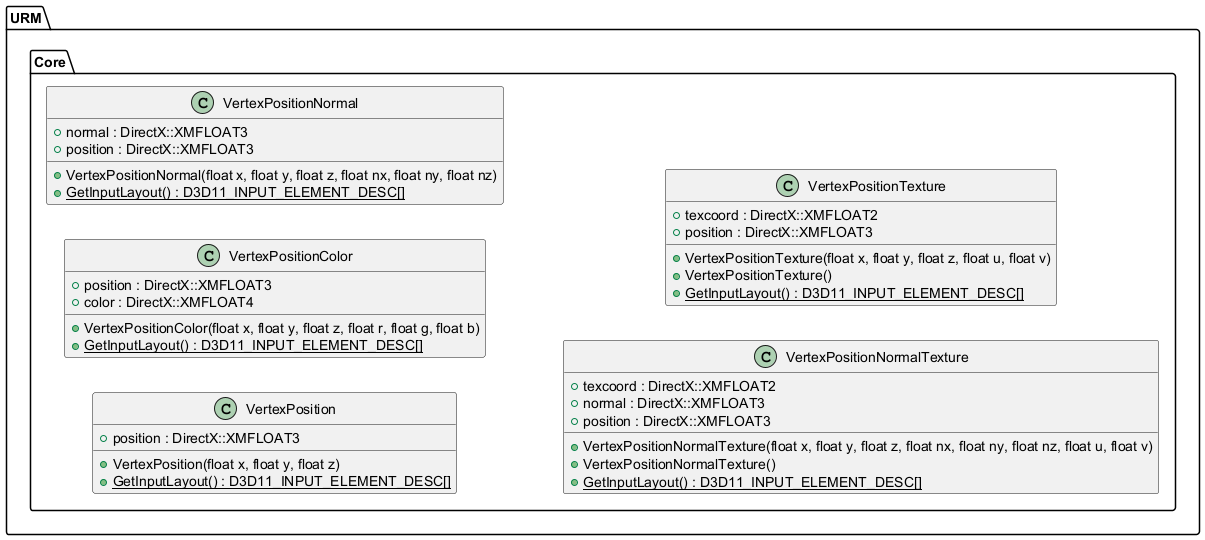
\includegraphics[width=\textwidth]{images/UML/vertextypes.png}
		\caption{Zaimplementowane standardowe typy wierzchołków.}
		\label{UML_VertexTypes}
	\end{figure}
	
	Do obsługi pozostałych typów wykorzystany został mechanizm \textit{concepts}, dodany w ramach standardu C++20 \cite{cpp20:concepts:2025}.
	Pozwala on na zdefiniowanie ograniczeń dla typu, co w opisywanym przypadku zostało wykorzystane do narzucenia konieczności implementacji statycznej metody \textit{std::vector<D3D11\_INPUT\_ELEMENT\_DESC> GetInputLayout()}, zwracającej wymaganą do poprawnej obsługi strukturę typu D3D11\_INPUT\_ELEMENT\_DESC.

	Dodatkowym elementem modularności jest obsługa modeli indeksowanych oraz nieindeksowanych, a także w razie potrzeby bezpośredni dostęp do wewnętrznych danych obiektu.
	
	Metadane przechowywane są jako lista wpisów typu \textbf{MaterialProperty}. Klasa ta obsługuje dane typów opisanych w enum \textbf{MaterialProperty::Types}, czyli typu buforowego, tekstowego \textit{(std::string)}, a także list liczb całkowitych \textit{(int)} i zmiennoprzecinkowych pojedynczej \textit{(float)} oraz podwójnej precyzji \textit{(double)}. Implementacja przechowuje te dane w postaci dynamicznie alokowanej i zwalnianej w destruktorze tablicy danych lub typu \textit{std::string}, a w celu zaoszczędzenia pamięci wykorzystany został moduł \textit{variant} ze standardu C++17 \cite{cpp17:variant:2025}. Przy pobieraniu danych następuje weryfikacja użycia poprawnego typu, który można sprawdzić używając metody \textit{GetType()}.
	
	\begin{figure}[h!]
		\centering
		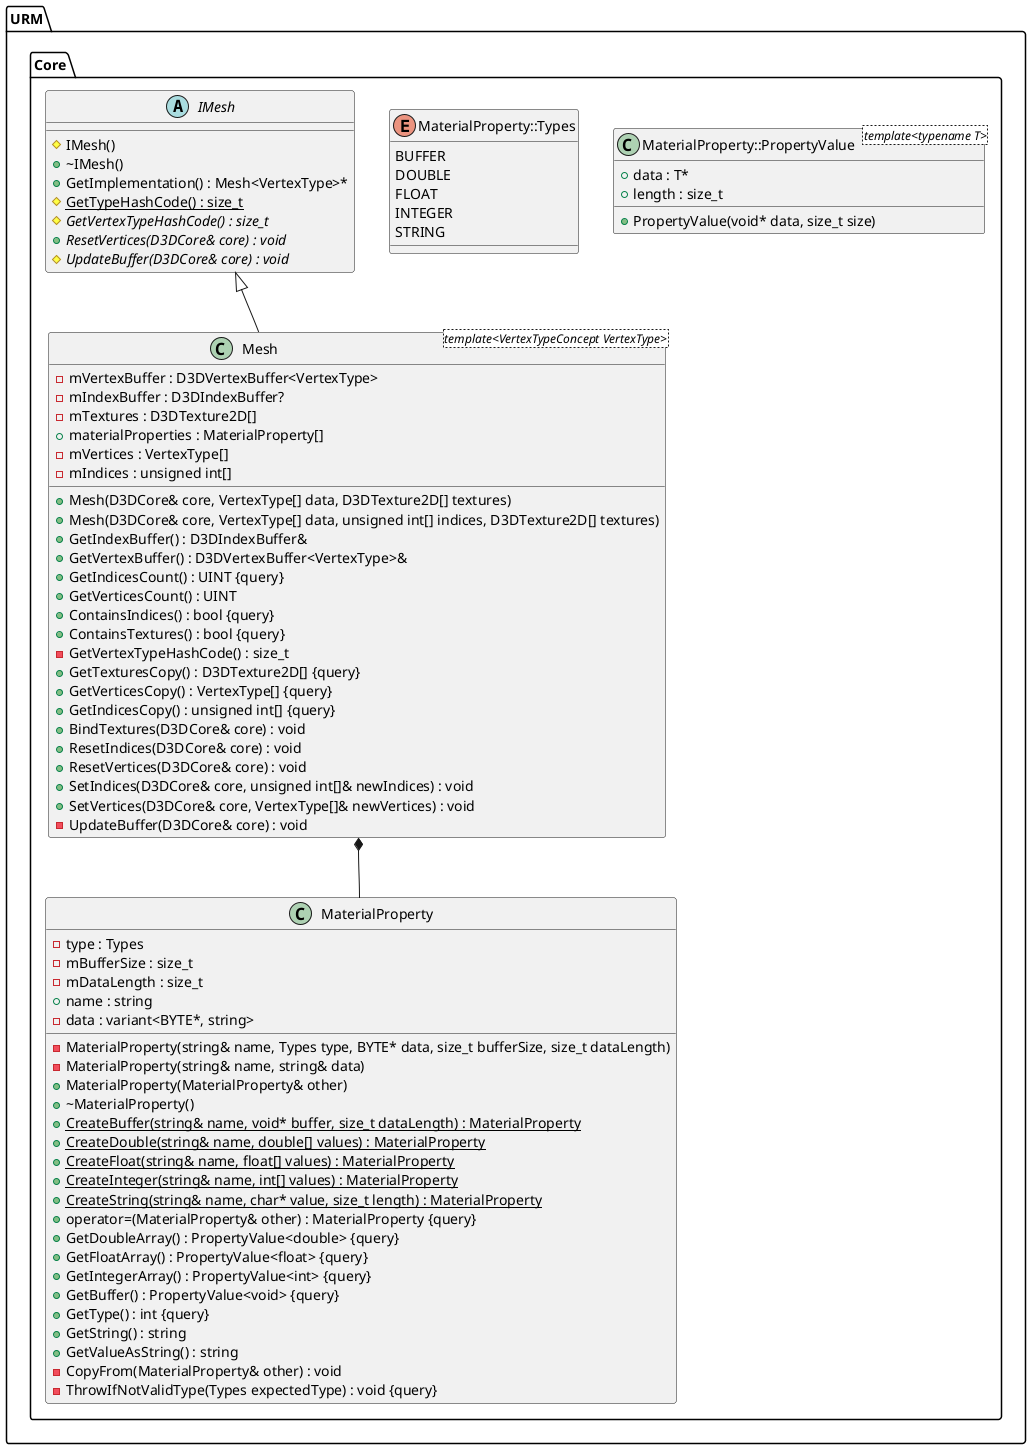
\includegraphics[width=\textwidth]{images/UML/mesh.png}
		\caption{Schemat klasy Mesh oraz klas wspierających.}
		\label{UML_Mesh}
	\end{figure}
	
		
	\vfill
	\clearpage
	
\subsection{Wczytywanie modeli}
	Funkcje pomocnicze ułatwiające wczytywanie modeli z pliku udostępnione zostały w ramach metod statycznych klasy \textbf{ModelLoader}. Metoda \textit{LoadFromFile()} jako argument otrzymuje ścieżkę do pliku modelu w obsługiwanym formacie, a następnie zwraca strukturę drzewową, której wierzchołkami są obiekty klasy \textbf{ModelLoaderNode}. Każdy wierzchołek zwracanego drzewa posiada macierz transformacji względem rodzica, listę mesh'y oraz wierzchołków przynależnych. Zachowywana zostaje oryginalna relacja transformacji między obiektami z wczytywanego pliku.
	Wraz z geometrią modelu wczytywane są także parametry metadanych do listy \textit{MaterialProperty} oraz przynależne do modelu tekstury. 
	
	Moduł obsługuje wszystkie formaty plików wspierane przez bibliotekę assimp, których pełna lista dostępna jest na stronie biblioteki \cite{github:assimp:FileFormats}. Szczególna uwaga została położona na wsparcie najczęściej spotykanych formatów, takich jak DAE, FBX, glTF / GLB, OBJ czy STL.
	
	Diagram opisywanych struktur został przedstawiony na rys. \ref{UML_ModelLoader}.
		
	\begin{figure}[h!]
		\centering
		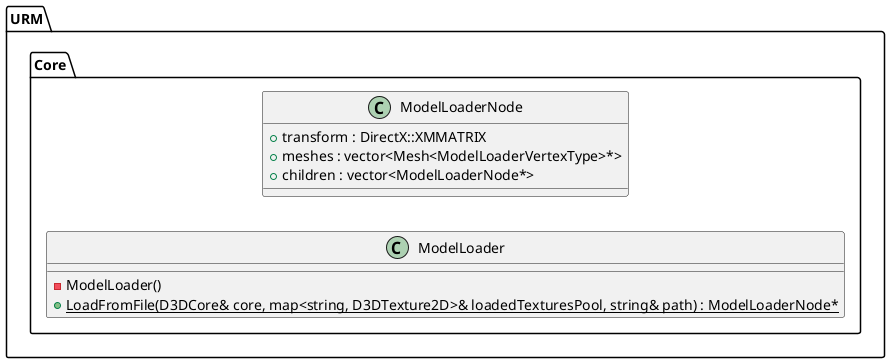
\includegraphics[width=\textwidth]{images/UML/modelloader.png}
		\caption{Schemat klasy statycznej ModelLoader wraz ze strukturą typu ModelLoaderNode.}
		\label{UML_ModelLoader}
	\end{figure}

\subsection{Tekstury}
	Kolejnym ważnym aspektem przy rysowaniu obiektów 3D są tekstury. Do reprezentacji ich dwuwymiarowych wersji powstała klasa \textbf{D3DTexture2D}, która przejmuje obowiązki wczytywania danych z pliku, utworzenia odpowiednich zasobów oraz zarządzania nimi. Istnieje także możliwość wczytania tekstury bezpośrednio z pamięci programu w formacie skompresowanym oraz nieskompresowanym.
	
	Do użycia z API D3D tekstury potrzebują także obiektu typu Sampler, który definiuje zachowanie próbkowania kolorów tekstury przy odczycie. Do ułatwienia tego zadania utworzona została klasa \textbf{D3DSampler}.
	
	Uproszczony schemat sekcji tekstur został opisany na rys. \ref{UML_Textures}.
	
	\begin{figure}[h!]
		\centering
		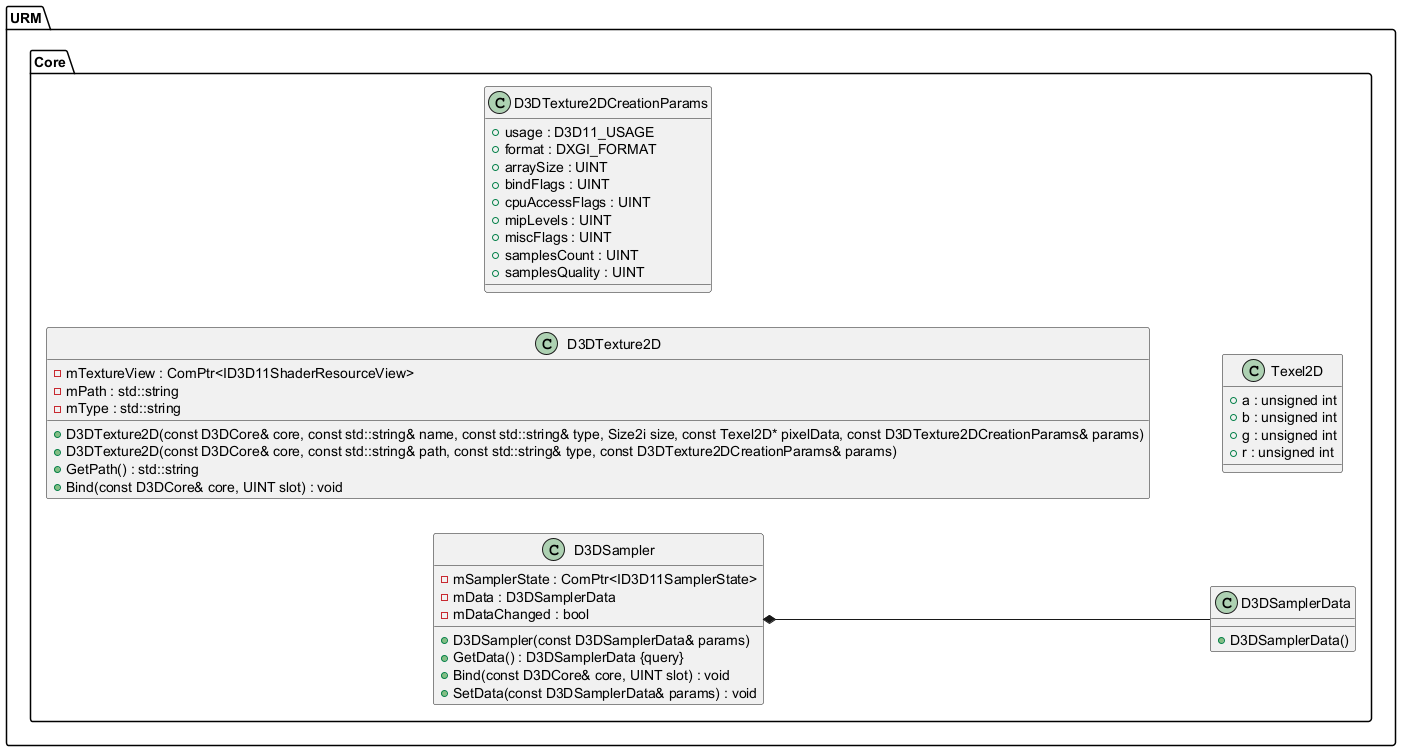
\includegraphics[width=\textwidth]{images/UML/texture.png}
		\caption{Schemat modułu tekstur.}
		\label{UML_Textures}
	\end{figure}
	
\subsection{Shader}
	W ramach modułu programy typy shader zostały zunifikowane do pojedynczej klasy, która reprezentuje poszczególne etapy procesu renderowania - \textbf{ShaderPipeline}. W aktualnej formie uwzględnia on etapy \textit{Vertex} oraz \textit{Pixel}, lecz dzięki modularnej budowanie możliwe jest uwzględnienie dodatkowych kroków, takich jak \textit{Geometry} czy \textit{Tesselation}.
	
	W ramach tego segmentu uwzględniony został także \textbf{D3DInputLayout}, służący jako warstwa abstrakcji nad układem wejściowym do shader'ów. Wykorzystuje on opisywany wcześniej koncept \textit{VertexTypeConcept} do automatycznego dopasowania w procesie rysowania modeli.
	
	Diagram UML segmentu został przedstawiony na rys. \ref{UML_ShaderPipeline}.
	
	\begin{figure}[h!]
		\centering
		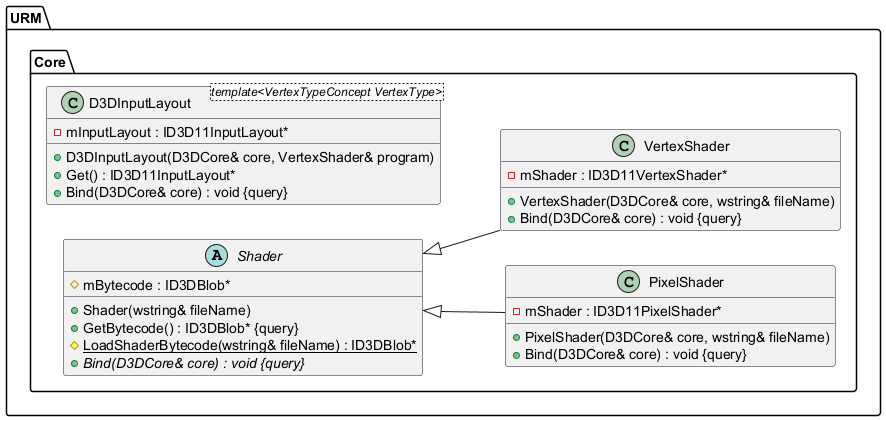
\includegraphics[width=\textwidth]{images/UML/shader.png}
		\caption{Schemat kompozycji klasy Shader oraz D3DInputLayout.}
		\label{UML_ShaderPipeline}
	\end{figure}
	\chapter{Przyjęta metoda rysowania sceny}
\label{ChapterSceneDrawingMethod}
	Ze względu na założenie uniwersalności - w tym pod względem platformy docelowej - jako podstawa i punkt wyjścia przyjęty został sposób rysowania \textit{Forward Rendering}, ze względu na lepszą skalowalność między systemami o różnej mocy obliczeniowej oraz możliwość użycia większości efektów graficznych. W związku z tym wyborem koszt obliczeniowy oraz pamięciowy rysowania sceny jest bazowo niski, lecz dodanie dużej ilości źródeł światła wiąże się ze zwiększonym narzutem obliczeniowym.
	
\section{Modyfikacja sposobu obliczania oświetlenia}
	Wyraźnym odejściem względem klasycznego \textit{Forward Rendering} jest sposób obliczania oświetlenia. Podstawową metodę można przedstawić w uproszczonej formie przy pomocy pseudokodu w ramach listingu \ref{lst:shaderForwardLightCalculations}.
	
	\begin{lstlisting}[caption={Pseudokod programu cieniującego obliczającego oświetlenie metodą Forward Rendering}, label={lst:shaderForwardLightCalculations}]
UNIFORM Light[] lights; // Przekazane do shader'a dane o źródłach światła,
UNIFORM int numLights;  // oraz o ilości aktywnych źródeł w tablicy.
		
Color resultColor = BLACK;
// Pętla sumująca obliczone wartości oświetlenia
for (i = 0; i < numLights; i += 1) {
    resultColor += CalculateLight(lights[i]);
}

return resultColor; 
	\end{lstlisting}
	
	Takie podejście ma jednak dwa ograniczenia - wydajność oraz ograniczenie maksymalnej ilości źródeł światła w scenie.	Pierwsze wynika ze sposobu działania współczesnych układów graficznych oraz kompilatorów. Dokładniej ograniczenie wydajności wynika z tzw. \textit{Register spilling}, czyli sytuacji w której na układzie graficznym brakuje rejestrów do pełnego pokrycia zmiennych, przez co koniecznym jest korzystanie z powolnej pamięci globalnej \cite{amd:gpuopen:RegisterSpilling}. Możliwym jest też spadek wydajności przez zmniejszenie skuteczności mechanizmu \textit{rozwijania pętli} kompilatora, przez znaczne zwiększenie maksymalnej jej długości. Drugie ograniczenie spowodowane jest limitem ilości elementów bufora stałych w API Direct3D - 4096 \cite{microsoft:Direct3D11:ResourceLimits}, co ogranicza ilość źródeł światła do około 1400. 
	
	Oba problemy zostały rozwiązane dzieląc pełną listę świateł na fragmenty o stałej wielkości (na przykład 64). Następnie zamiast wywoływać proces renderowania dla wszystkich źródeł, uruchamiany jest po kolei dla kolejnych segmentów, a wynik dodawany jest do bufora kolorów przy pomocy mechanizmu \textit{Blending}, opartego o klasę z segmentu \textit{D3DBlendState}. Aby takie podejście działało poprawnie pierwsze wywołanie procesu rysującego odbywa się przy wyłączonym blendingu.
	
	Nowe podejście także może zmniejszać wydajność przy zbyt małej ilości źródeł światła na wywołanie procesu ze względu na konieczność każdorazowego rysowania geometrii i zmiany kontekstów. W związku z tym przeprowadzone zostały testy, z których została określona optymalna wartość świateł na pass - \textbf{64}.
	
	Wizualizacja procesu została pokazana na rys. \ref{Rendering_MultiPassLighting}.
	
		
	\begin{figure}[h!]
		\centering
		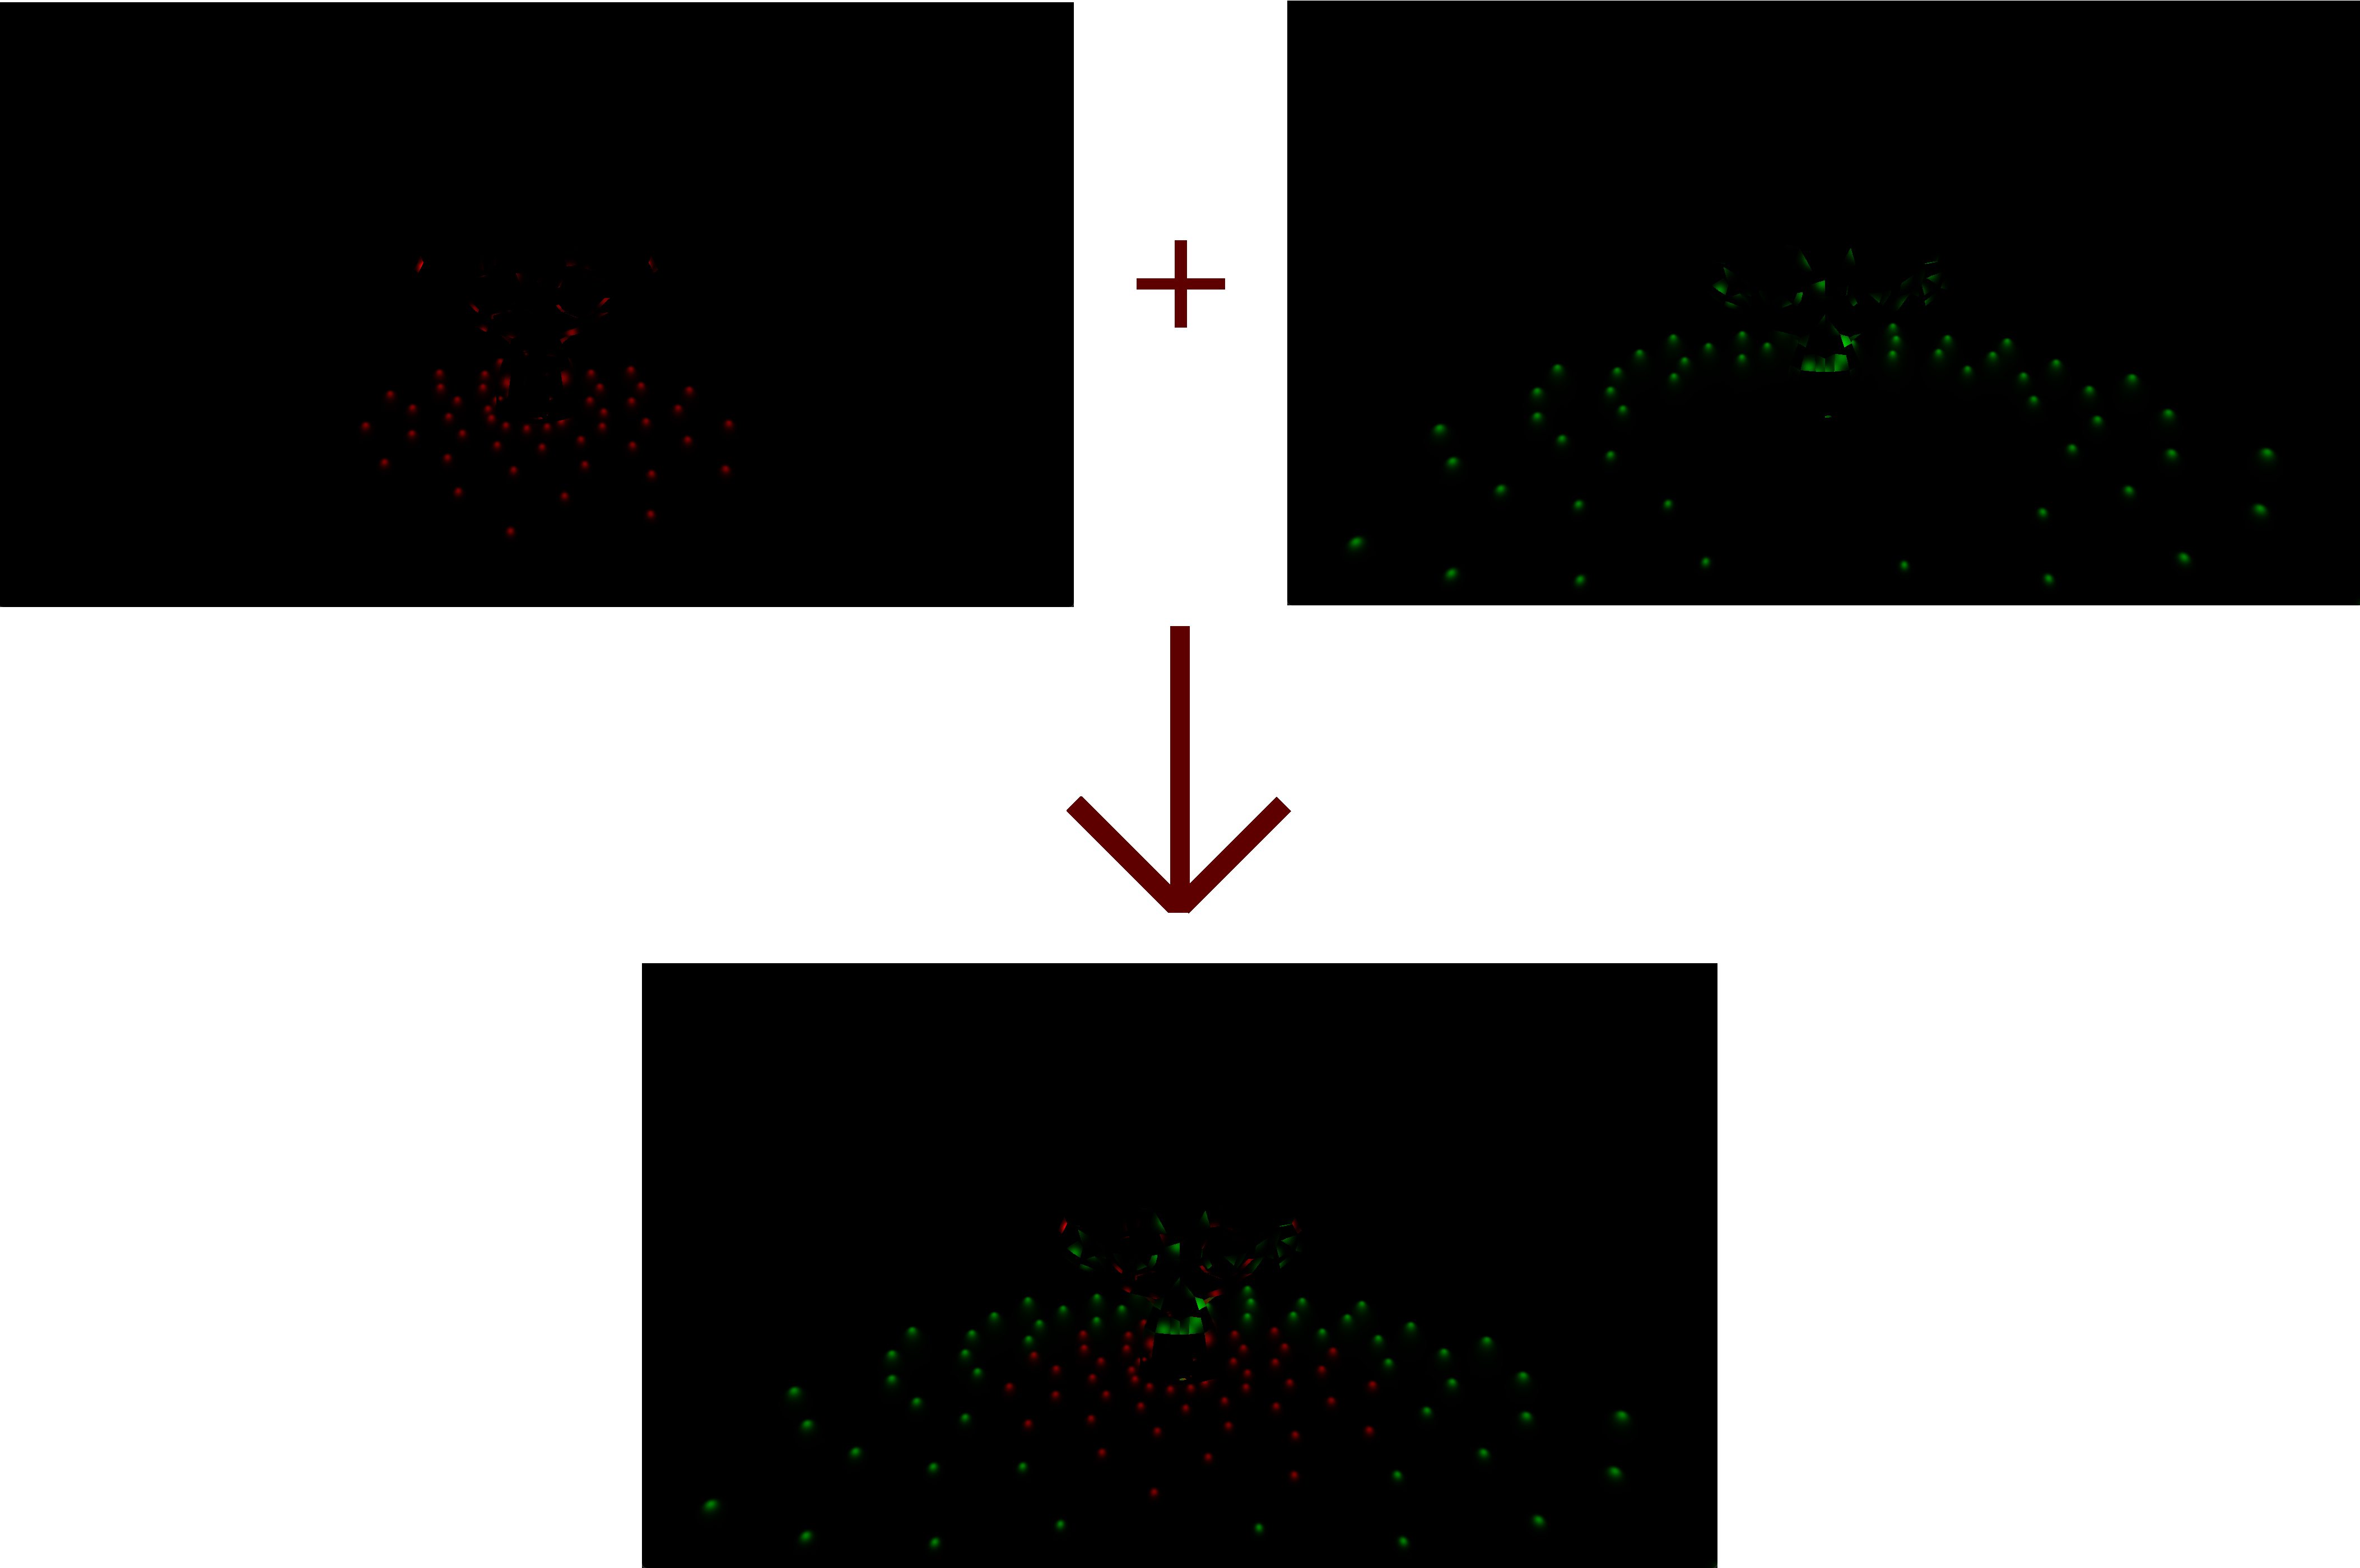
\includegraphics[width=\textwidth]{images/lightsTest_combined.png}
		\caption{Wizualizacja procesu wieloetapowego obliczania oświetlenia.}
		\label{Rendering_MultiPassLighting}
	\end{figure}
	\chapter{Testy modułu}
	
	\iffalse
		Testy:
			- Porównanie dla trybu "Natywnego", "URM::Core", "URM::Engine".
			- Porównanie złożoności kodu.
			1) Wydajność przetwarzania wierzchołków.
				* Testy wyświetlania obiektów o bardzo złożonej topologii.
				- Oszacowanie maksymalnej ilości wierzchołków.
				- Sprawdzenie narzutu na CPU i GPU.
				+ Optymalizacje vertex shader'a.
				
			2) Wydajność generowania oświetlenia
				* Sprawdzenie narzutu wydajności wielu źródeł światła.
				- Oszacowanie maksymalnego limitu ilości świateł w scenie.
				+ Dodanie bardziej zaawansowanego silnika obliczania efektów oświetlenia.
				
			3) Testy wydajności pixel shader'a.
				- Sprawdzenia skalowania wydajności zależnie od rozdzielczości.
				- Sprawdzenie bottleneck'u (CPU / GPU).
				
			4) Instance rendering.
				- Sprawdzenie jak moduł radzi sobie z rysowaniem wielu instancji tego samego lub różnych obiektów.
				- Porównanie wydajności z różnymi shader'ami i tym samym shader'em.
				
			5) Wydajność wczytywania modeli i tekstur z pliku.
				- Porównanie różnych formatów.
				- Porównanie różnych opcji preprocessingu.
				- Porównanie pierwszego i kolejnych wczytań modelu (AssetManager).
				
			6) Testy wydajności macierzy transformacji w Transform.
				- Określenie złożoności obliczeniowej poszczególnych funkcji.
				- Oszacowanie maksymalnej głębokości oraz szerokości drzewa obiektów.
				- Sprawdzenie narzutu wielokrotnego ustalania pozycji.
				+ Cache'ing.
				
	\fi
	
	Do lepszego zrozumienia oraz wykorzystania nowo powstałej biblioteki warto znać jej lepsze oraz słabsze strony, a także teoretyczne i praktyczne ograniczenia. W związku z tym przeprowadzone zostały testy różnych aspektów omawianego projektu, aby ustalić limity ilościowe i wydajnościowe, a także ich przyczyny w celu opracowania możliwości ich poprawy.
	
	\section{Framework testowy}
	Do łatwiejszego tworzenia testów utworzona została abstrakcyjna klasa interfejs - \textbf{ITest}, która ujednolica API testów do późniejszego wykorzystania. Obiekty dziedziczące implementują metody \textit{OnInit()} do inicjalizacji oraz \textit{OnUpdate()} do aktualizacji co klatkę obrazu.
	
	Podzbiorem testów są także pomiary wydajności i/lub limitu ilości testowanego parametru. Do obsługi tego zbioru oddana została druga klasa - \textbf{AutoTest}. Dziedziczy ona z \textit{ITest}, ale zastępuje \textit{Init()} i \textit{Update()}, pozostawiając opisane już metody abstrakcyjne do implementacji przez klasy dziedziczące. Różnicą względem rodzica jest próba automatycznego dopasowania złożoności testu do założonego poziomu wydajności. 
	
	\subsection{Metoda określania wydajności przez AutoTest}
	Każdy oparty o \textit{AutoTest} skrypt musi posiadać wartość mierzalną, nazwaną w uproszczeniu ilością (\textit{count}). Zwiększenie tej wartości powinno z założenia liniowo zmniejszać wydajność renderowania, a co za tym idzie zwiększać czas generowania klatki obrazu. Informacja o długości rysowania jest następnie agregowana przez 100 wpisów przy pomocy obiektu klasy \textbf{AverageAccumulator} do wartości średniej, która zostaje przyrównana z czasem oczekiwanym, definiowanym przez test za pomocą metody \textit{GetTargetFPS()}. Na podstawie wzajemnej proporcji tych wartości obliczana jest teoretyczna ilość potrzebnych do dodania elementów, aby osiągnąć zamierzony cel. Przed aplikacją za pomocą funkcji \textit{IncreaseCount()}, ilość zostaje pomniejszona przez pomnożenie o wartość z wirtualnej metody \textit{GetTargetCurveMultiplier()}, aby zmniejszyć prawdopodobieństwo przeszacowania celu. Cykl ten powtarzany jest aż do zejścia czasu rysowania klatki poniżej progu. Następnym krokiem jest stopniowa reprodukcja operacji, ale zmniejszając ilość o 1 za pomocą \textit{DecreaseCount()}, aż do ponownego przekroczenia docelowej długości renderowania w 3 bezpośrednio następujących po sobie pomiarach. Taka forma pomiaru pozwala na powtarzalne określenie maksymalnej ilości elementów spełniających założony cel wydajnościowy. Wykres czasu klatki z przykładowego testu oświetlenia został przedstawiony w całości na rys. \ref{Test_LightsTest_FullFrameTime} oraz ograniczony do partii autoregulacji na rys. \ref{Test_LightsTest_AutoFrameTime}.
	
	\begin{figure}[h!]
		\begin{subfigure}{.5\textwidth}
			\centering
			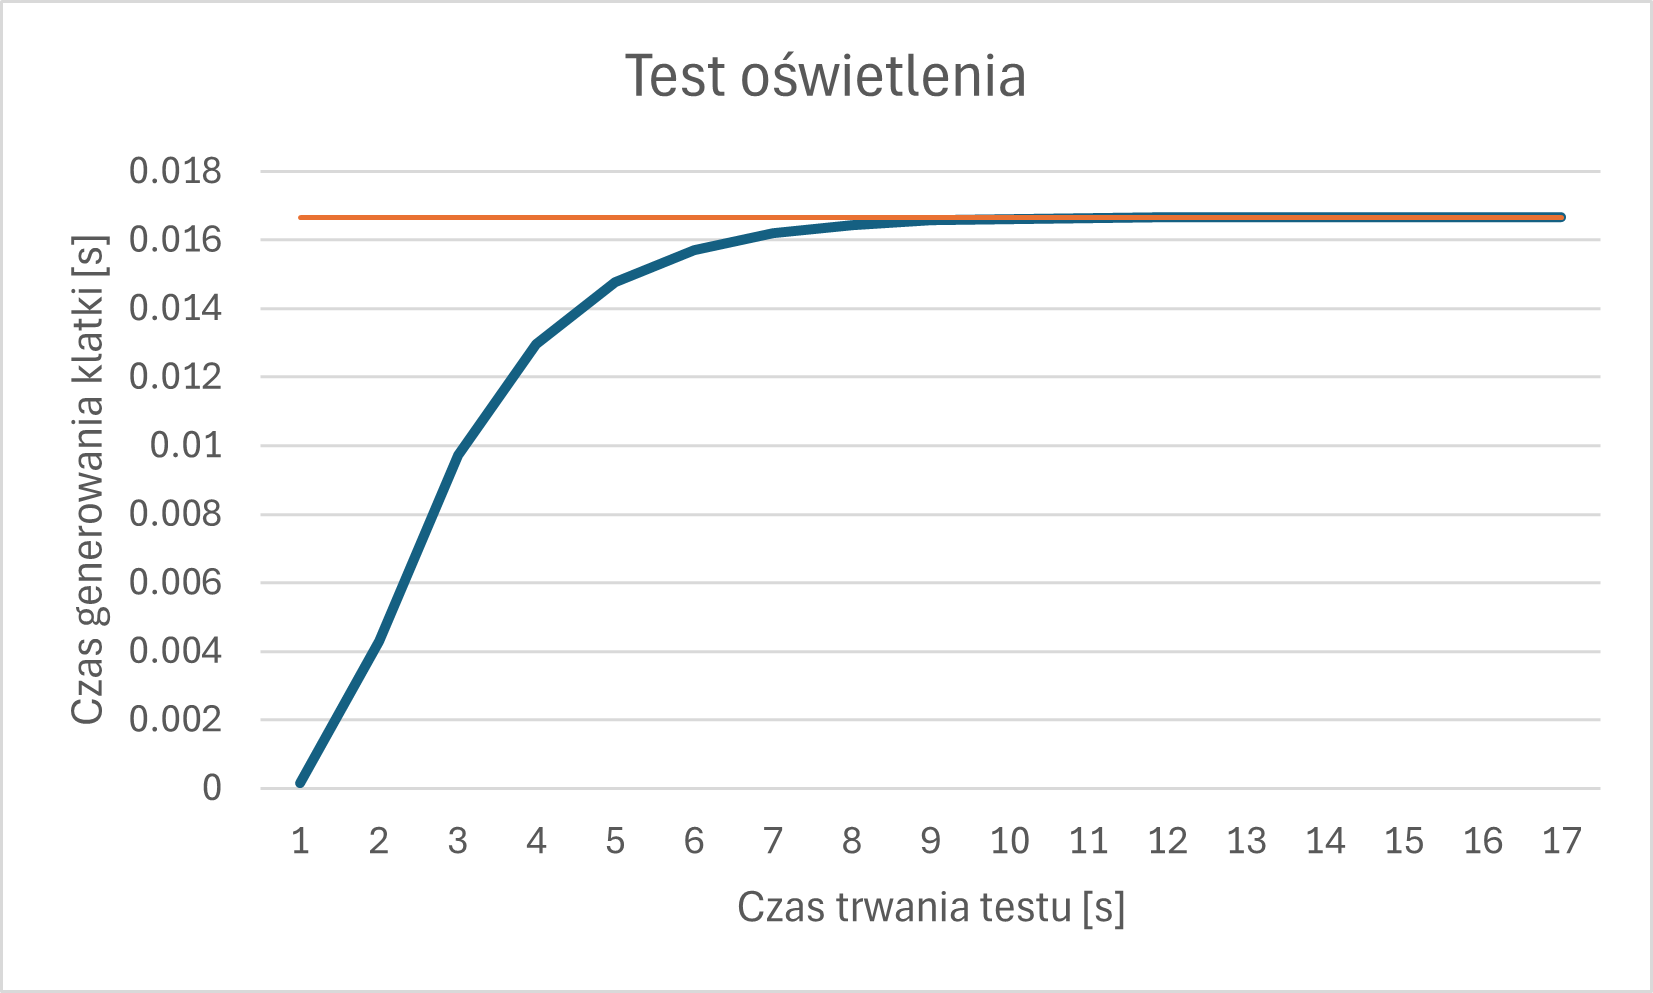
\includegraphics[width=\textwidth]{images/LightsTestResult_full.png}
			\caption{Pełny wykres czasu generowania klatki.}
			\label{Test_LightsTest_FullFrameTime}
		\end{subfigure}
		\begin{subfigure}{.5\textwidth}
			\centering
			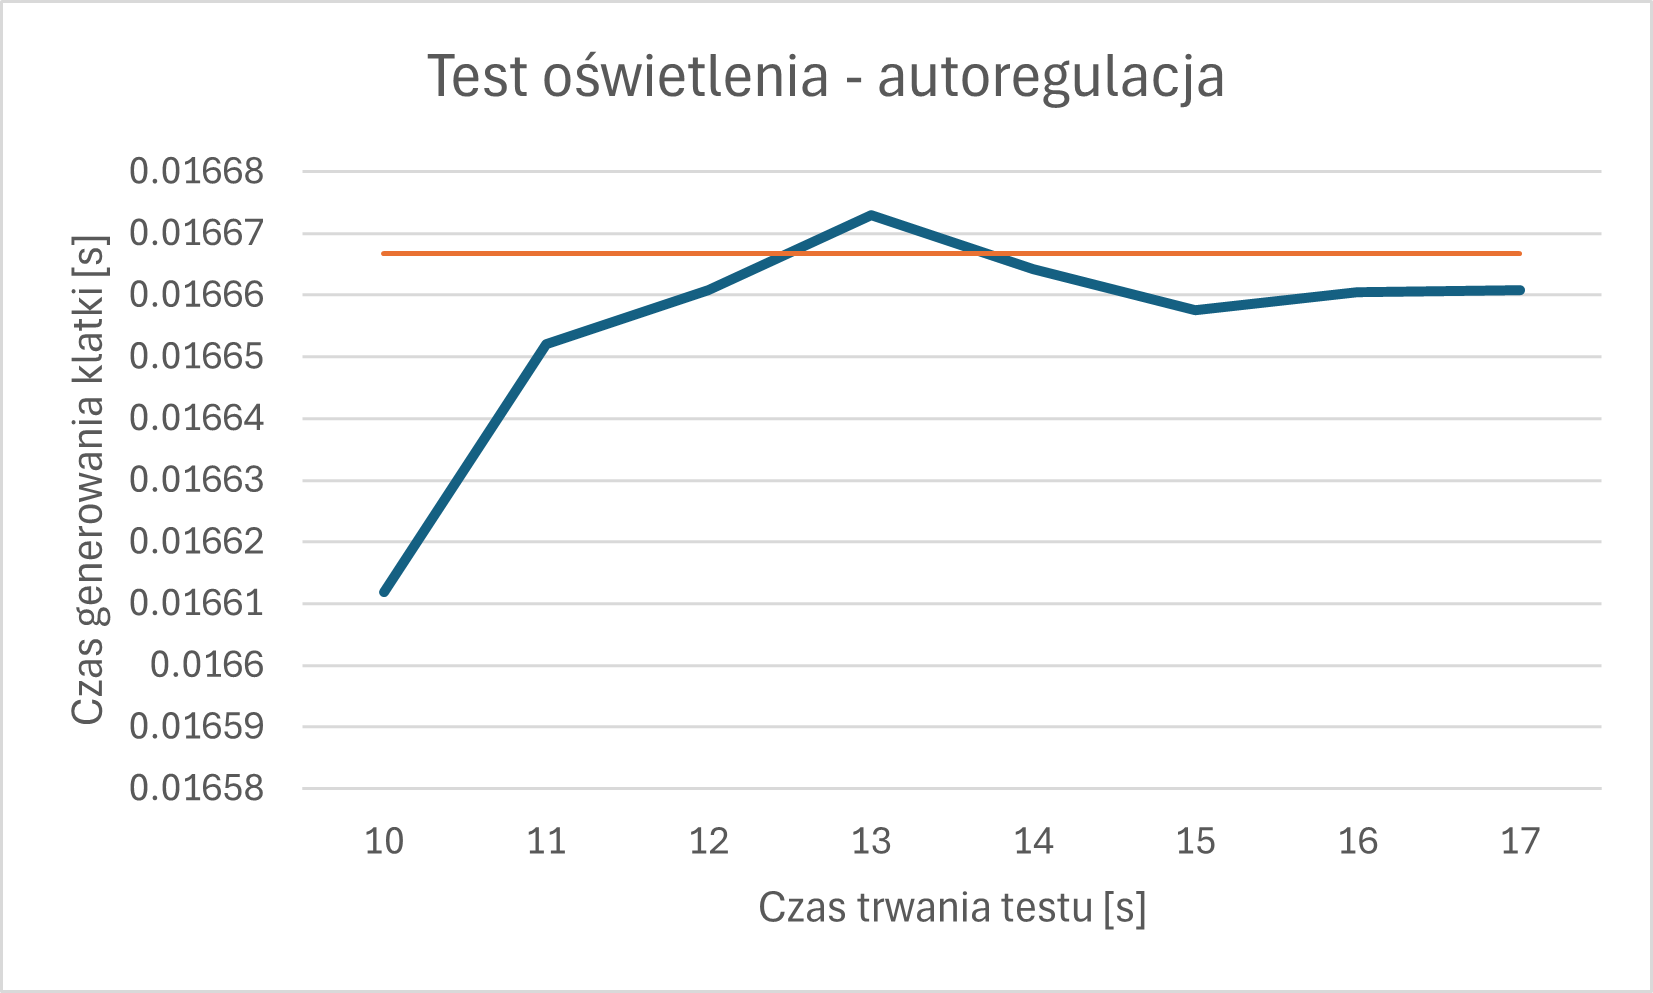
\includegraphics[width=\textwidth]{images/LightsTestResult_auto.png}
			\caption{Czas rysowania obrazu ograniczony do fragmentu autoregulacji.}
			\label{Test_LightsTest_AutoFrameTime}
		\end{subfigure}
		\caption{Wykres pokazujący działanie mechanizmu \textit{AutoTest} podczas testu oświetlenia.}
	\end{figure}
	
	\subsection{Eliminacja błędów}
	Aby test był wiarygodny należy zabezpieczyć go na wypadek wystąpienia różnego rodzaju błędów. Poniżej przedstawiona została lista potencjalnych problemów oraz podjęte działania w celu ich eliminacji.
	\begin{itemize}
		\item \textbf{Anomalie pomiaru} - generowanie klatek obrazu nie zawsze odbywa się całkowicie stabilnie. Skokowe obciążenie systemu procesem w tle, nieprzewidziane zwalnianie zasobów przez system operacyjny, a nawet błędy sprzętowe mogą powodować skok czasu generowania pojedynczych klatek obrazu. Takie pomiary eliminowane są przy pomocy algorytmu IQR, służącego do wykrywania anomalii, w tym przypadku przyjmujących formę czasu wyraźnie odbiegającego od pozostałych pomiarów. Taki sposób filtracji jest możliwy ze względu na obraną metodę, która powinna generować niezmienną wartość pomiarów między zmianami ilości.
		\item \textbf{Wpływ dodawania elementów na czas generowania klatki} - alokacja i inicjalizacja dużej ilości obiektów może generować wyraźne spadki wydajności w ramach pojedynczej klatki. Zostały zaimplementowane dwa mechanizmy mające na celu obronę przed taką sytuacją. Pierwszym jest opisany już IQR, który powinien eliminować wyraźne anomalie. Drugi to zatrzymanie czasomierza w \textit{AverageAccumulator} na czas przetwarzania wyników pomiarów (w tym ewentualne zwiększenie bądź zmniejszenie ilości elementów), a następne wznowienie już po wykonaniu opisanych czynności. 
		\item \textbf{Przeszacowanie zwiększenia ilości elementów} - mechanizm odpowiedzialny za ograniczenie takiej sytuacji został już opisany i jest nim podejście, w którym najpierw szacunkowo zostaje określona ilość powodująca spadek wydajności poniżej progu, aby potem bardzo powolną redukcją nastąpiło określenie wartości docelowej. Dodatkowym sposobem jest nadpisywalna metoda \textit{GetTargetCurveMultiplier()}, dzięki której bardziej złożone testy mogą zmniejszyć prawdopodobieństwo przeszacowania, kosztem zwiększonego czasu trwania testu.
		\item \textbf{Niedokładność czasu pomiaru} - użycie klasy \textit{high\_resolution\_clock} ze standardowej biblioteki C++ umożliwia dokonywanie pomiaru czasu z bardzo wysoką precyzją liczoną w nanosekundach.
	\end{itemize}
	
	\section{Testy wydajności}
	Poniżej przedstawione zostały zaimplementowane testy wydajności wraz z krótkim opisem, porównaniem działania między systemami testowymi oraz analizą z czego wynikają jego ograniczenia.
    \chapter{Decyzje projektowe, wybór API}

% % Definicja kolorów dla listingu kodu
% \definecolor{codegreen}{rgb}{0,0.6,0}
% \definecolor{codegray}{rgb}{0.5,0.5,0.5}
% \definecolor{codepurple}{rgb}{0.58,0,0.82}
% \definecolor{backcolour}{rgb}{0.95,0.95,0.92}
% \definecolor{keywordblue}{rgb}{0,0,1}

% % Definicja stylu C++ dla pakietu listings
% % Używamy mathescape=true, aby oryginalne komendy LaTeX w kodzie (np. \emph) były renderowane
% \lstdefinestyle{cppstyle}{
% 	language=C++,
% 	backgroundcolor=\color{backcolour},
% 	commentstyle=\color{codegreen},
% 	keywordstyle=\color{magenta},
% 	numberstyle=\tiny\color{codegray},
% 	stringstyle=\color{codepurple},
% 	basicstyle=\ttfamily\footnotesize,
% 	breakatwhitespace=false,
% 	breaklines=true,
% 	captionpos=b,
% 	keepspaces=true,
% 	numbers=left,
% 	numbersep=5pt,
% 	showspaces=false,
% 	showstringspaces=false,
% 	showtabs=false,
% 	tabsize=2,
% 	mathescape=true, % Pozwala na używanie $...$ do wstawiania komend LaTeX w kodzie
% 	morekeywords={*,ComPtr,hwnd,message,wParam,lParam,uint,LRESULT,CALLBACK,HWND,UINT,IDirect3D9,Direct3DCreate9,D3D_SDK_VERSION,D3DPRESENT_PARAMETERS,Windowed,SwapEffect,D3DSWAPEFFECT_DISCARD,hDeviceWindow,BackBufferFormat,D3DFMT_UNKNOWN,EnableAutoDepthStencil,AutoDepthStencilFormat,D3DFMT_D16,IDirect3DDevice9,CreateDevice,D3DADAPTER_DEFAULT,D3DDEVTYPE_HAL,D3DCREATE_SOFTWARE_VERTEXPROCESSING,D3DCREATE_HARDWARE_VERTEXPROCESSING,D3DDEVTYPE_REF,E_FAIL,HRESULT,FAILED,SUCCEEDED,S_OK,Vertex,DWORD,D3DFVF_CUSTOMVERTEX,D3DFVF_XYZRHW,D3DFVF_DIFFUSE,IDirect3DVertexBuffer9,CreateVertexBuffer,D3DUSAGE_WRITEONLY,D3DPOOL_DEFAULT,Lock,memcpy,Unlock,SetRenderState,D3DRS_CULLMODE,D3DCULL_NONE,D3DRS_LIGHTING,FALSE,D3DRS_ZENABLE,TRUE,Clear,D3DCLEAR_TARGET,D3DCLEAR_ZBUFFER,D3DCOLOR_XRGB,BeginScene,SetFVF,SetStreamSource,sizeof,DrawPrimitive,D3DPT_TRIANGLELIST,EndScene,Present,D3DERR_DEVICELOST,D3DERR_DEVICENOTRESET,TestCooperativeLevel,Reset,ID3D11Device,ID3D11DeviceContext,IDXGISwapChain,ID3D11RenderTargetView,ID3D11DepthStencilView,ID3D11Texture2D,depthStencilBuffer,ID3D11VertexShader,ID3D11PixelShader,ID3D11InputLayout,ID3D11Buffer,windowWidth,windowHeight,DXGI_SWAP_CHAIN_DESC,BufferCount,BufferDesc,Width,Height,Format,DXGI_FORMAT_R8G8B8A8_UNORM,RefreshRate,Numerator,Denominator,BufferUsage,DXGI_USAGE_RENDER_TARGET_OUTPUT,OutputWindow,SampleDesc,Count,Quality,D3D_FEATURE_LEVEL,D3D_FEATURE_LEVEL_11_0,featureLevel,D3D11CreateDeviceAndSwapChain,D3D_DRIVER_TYPE_HARDWARE,D3D_DRIVER_TYPE_WARP,D3D11_CREATE_DEVICE_DEBUG,D3D11_SDK_VERSION,GetBuffer,__uuidof,LPVOID,CreateRenderTargetView,D3D11_TEXTURE2D_DESC,MipLevels,ArraySize,DXGI_FORMAT_D24_UNORM_S8_UINT,D3D11_USAGE_DEFAULT,BindFlags,D3D11_BIND_DEPTH_STENCIL,CPUAccessFlags,MiscFlags,CreateTexture2D,CreateDepthStencilView,OMSetRenderTargets,GetAddressOf,D3DCompile,strlen,nullptr,ID3DBlob,errorBlob,vs_5_0,ps_5_0,D3DCOMPILE_ENABLE_STRICTNESS,GetBufferPointer,GetBufferSize,CreateVertexShader,CreatePixelShader,D3D11_INPUT_ELEMENT_DESC,POSITION,COLOR,DXGI_FORMAT_R32G32B32_FLOAT,DXGI_FORMAT_R32G32B32A32_FLOAT,D3D11_INPUT_PER_VERTEX_DATA,D3D11_APPEND_ALIGNED_ELEMENT,ARRAYSIZE,CreateInputLayout,D3D11_BUFFER_DESC,Usage,D3D11_USAGE_IMMUTABLE,D3D11_BIND_VERTEX_BUFFER,D3D11_SUBRESOURCE_DATA,pSysMem,CreateBuffer,D3D11_VIEWPORT,MinDepth,MaxDepth,TopLeftX,TopLeftY,RSSetViewports,ClearRenderTargetView,ClearDepthStencilView,D3D11_CLEAR_DEPTH,D3D11_CLEAR_STENCIL,IASetVertexBuffers,stride,offset,IASetInputLayout,IASetPrimitiveTopology,D3D11_PRIMITIVE_TOPOLOGY_TRIANGLELIST,VSSetShader,PSSetShader,Draw,DXGI_ERROR_DEVICE_REMOVED,DXGI_ERROR_DEVICE_RESET,OnDeviceLost,ID3D12Device,IDXGIFactory6,ID3D12CommandQueue,IDXGISwapChain3,ID3D12DescriptorHeap,rtvDescriptorSize,ID3D12Resource,ID3D12CommandAllocator,ID3D12RootSignature,ID3D12PipelineState,ID3D12GraphicsCommandList,D3D12_VERTEX_BUFFER_VIEW,ID3D12Fence,UINT64,HANDLE,FrameCount,fenceValues,fenceEvent,exception,std,ThrowIfFailed,DXGI_CREATE_FACTORY_DEBUG,CreateDXGIFactory2,IDXGIAdapter1,GetHardwareAdapter,D3D12CreateDevice,D3D12_COMMAND_QUEUE_DESC,Type,D3D12_COMMAND_LIST_TYPE_DIRECT,Flags,D3D12_COMMAND_QUEUE_FLAG_NONE,CreateCommandQueue,DXGI_SWAP_CHAIN_DESC1,SwapEffect,DXGI_SWAP_EFFECT_FLIP_DISCARD,IDXGISwapChain1,CreateSwapChainForHwnd,MakeWindowAssociation,DXGI_MWA_NO_ALT_ENTER,As,GetCurrentBackBufferIndex,D3D12_DESCRIPTOR_HEAP_DESC,NumDescriptors,D3D12_DESCRIPTOR_HEAP_TYPE_RTV,D3D12_DESCRIPTOR_HEAP_FLAG_NONE,CreateDescriptorHeap,GetDescriptorHandleIncrementSize,D3D12_CPU_DESCRIPTOR_HANDLE,rtvHandle,GetCPUDescriptorHandleForHeapStart,ptr,CreateCommandAllocator,D3D12_ROOT_SIGNATURE_DESC,Init,D3D12_ROOT_SIGNATURE_FLAG_ALLOW_INPUT_ASSEMBLER_INPUT_LAYOUT,D3D_ROOT_SIGNATURE_VERSION_1,D3D12SerializeRootSignature,CreateRootSignature,D3D12_INPUT_ELEMENT_DESC,D3D12_GRAPHICS_PIPELINE_STATE_DESC,InputLayout,pRootSignature,VS,PS,CD3DX12_SHADER_BYTECODE,CD3DX12_RASTERIZER_DESC,CD3DX12_BLEND_DESC,CD3DX12_DEPTH_STENCIL_DESC,PrimitiveTopologyType,D3D12_PRIMITIVE_TOPOLOGY_TYPE_TRIANGLE,NumRenderTargets,RTVFormats,DSVFormat,DXGI_FORMAT_D32_FLOAT,SampleMask,UINT_MAX,CreateGraphicsPipelineState,CreateCommandList,Close,vertexBufferSize,D3D12_HEAP_PROPERTIES,CD3DX12_HEAP_PROPERTIES,D3D12_HEAP_TYPE_DEFAULT,D3D12_RESOURCE_DESC,CD3DX12_RESOURCE_DESC,Buffer,CreateCommittedResource,D3D12_HEAP_FLAG_NONE,D3D12_RESOURCE_STATE_COPY_DEST,D3D12_HEAP_TYPE_UPLOAD,D3D12_RESOURCE_STATE_GENERIC_READ,Map,UINT8,pVertexDataBegin,reinterpret_cast,CD3DX12_RANGE,Unmap,Reset,CopyBufferRegion,D3D12_RESOURCE_BARRIER,CD3DX12_RESOURCE_BARRIER,Transition,D3D12_RESOURCE_STATE_VERTEX_AND_CONSTANT_BUFFER,ResourceBarrier,ExecuteCommandLists,_countof,ppCommandLists,BufferLocation,GetGPUVirtualAddress,StrideInBytes,SizeInBytes,CreateFence,D3D12_FENCE_FLAG_NONE,CreateEvent,GetLastError,HRESULT_FROM_WIN32,WaitForGpu,PopulateCommandList,SetPipelineState,SetGraphicsRootSignature,SetDescriptorHeaps,CD3DX12_VIEWPORT,static_cast,CD3DX12_RECT,RSSetViewports,RSSetScissorRects,D3D12_RESOURCE_STATE_PRESENT,D3D12_RESOURCE_STATE_RENDER_TARGET,CD3DX12_CPU_DESCRIPTOR_HANDLE,OMSetRenderTargets,ClearRenderTargetView,IASetPrimitiveTopology,D3D_PRIMITIVE_TOPOLOGY_TRIANGLELIST,IASetVertexBuffers,DrawInstanced,Signal,GetCompletedValue,SetEventOnCompletion,WaitForSingleObjectEx,previousFrameIndex,CleanupD3D12,CloseHandle,stbi_load,stbi_image_free,stbi_failure_reason,vector,unsigned,char,data,resize,size_t,cerr,cout,wcout,wcerr,endl,hex,WICTextureLoader,CreateWICTextureFromFile,textureResource,textureView,GetDesc,Reset,EffectFactory,Model,CreateFromCMO,CreateFromSDKMESH,wcsstr,meshes,CommonStates,Draw,CXMMATRIX,Assimp,Importer,ReadFile,aiProcess_Triangulate,aiProcess_GenSmoothNormals,aiProcess_FlipUVs,aiProcess_JoinIdenticalVertices,aiProcess_CalcTangentSpace,aiProcess_OptimizeMeshes,aiProcess_OptimizeGraph,aiScene,mFlags,AI_SCENE_FLAGS_INCOMPLETE,mRootNode,GetErrorString,processNode,aiNode,mMeshes,mNumMeshes,push_back,processMesh,aiMesh,mNumChildren,mChildren,MeshData,materialIndex,name,C_Str,vertices,indices,reserve,mNumVertices,XMFLOAT3,XMFLOAT2,XMFLOAT4,mVertices,HasNormals,mNormals,mTextureCoords,mNumFaces,aiFace,mFaces,mNumIndices,substr,find_last_of,directory,processMaterials,ModelData,renderModelAssimp,DrawIndexed,Vector3,Matrix,Quaternion,XMVECTOR,XMMATRIX,SimpleMath}
% }

% % Definicja stylu C# dla pakietu listings
% % Zmieniono tylko na C++, zgodnie z poleceniem, ale zachowujemy oryginalną treść
% \lstdefinestyle{csharpstyle}{
% 	language=C++, % Używamy C++ zgodnie z poleceniem, nawet dla kodu C#
% 	backgroundcolor=\color{backcolour},
% 	commentstyle=\color{codegreen},
% 	keywordstyle=\color{keywordblue}, % Niebieski dla odróżnienia
% 	numberstyle=\tiny\color{codegray},
% 	stringstyle=\color{codepurple},
% 	basicstyle=\ttfamily\footnotesize,
% 	breakatwhitespace=false,
% 	breaklines=true,
% 	captionpos=b,
% 	keepspaces=true,
% 	numbers=left,
% 	numbersep=5pt,
% 	showspaces=false,
% 	showstringspaces=false,
% 	showtabs=false,
% 	tabsize=2,
% 	mathescape=true, % Pozwala na używanie $...$ do wstawiania komend LaTeX w kodzie
% 	morekeywords={Device,VertexBuffer,Control,PresentParameters,SwapEffect,CreateFlags,CustomVertex,PositionColored,GraphicsStream,LockFlags,Usage,Pool,ClearFlags,System,Drawing,Color,PrimitiveType,Microsoft,DirectX,Direct3D,using,new,typeof,WriteOnly,Format,Default,Write,var,float,int,void,class,struct,enum,namespace,public,private,protected,static,readonly,get,set,true,false,null,return,if,else,for,foreach,while,do,switch,case,default,break,continue,try,catch,finally,throw,Form,ClientSize,Text,Show,DirectXException,MessageBox,Disposed,TestCooperativeLevel,DeviceLostException,Console,WriteLine,ToArgb,PaintEventHandler,PaintEventArgs,object,sender,Size,DepthFormat,D16,RenderState,CullMode,Cull,Lighting,ZBufferEnable,DeviceNotResetException}
% }

% \lstset{style=cppstyle} % Ustaw domyślny styl na C++

% % Definicja \real (jeśli nie jest zdefiniowana gdzie indziej)
% \providecommand{\real}[1]{#1}

Przed przystąpieniem do pisania kodu konieczne jest zbadanie dostępnych
na rynku API, które wejdą w skład projektowanego pakietu. Dla
opisywanego programu koniecznym jest między innymi dobranie oraz
przetestowanie różnych wersji API Direct3D, wybór języka programowania,
bibliotek służących do zaawansowanych obliczeń matematycznych, wejścia z
klawiatury i kontrolera, a także bibliotek pomocniczych do otwierania
okna renderowania. Decyzja powinna być oparta o testy wydajności,
wsparcie platformy docelowej, jakość dokumentacji, jak i o bilans
możliwości do złożoności API.

% Usunięto błędną strukturę enumerate->enumerate
\section{API obsługi okna}

Zanim zostaną podjęte jakiekolwiek decyzje na temat rysowania grafiki,
należy mieć otwarte oraz skonfigurowane okno w taki sposób, aby było na
czym obraz rysować. Testy tego aspektu polegały na stworzeniu minimalnego kodu otwierającego
okno zdolne do wyświetlania grafiki narysowanej z wykorzystaniem DirectX.

\subsection{SDL2}

Skrót od \emph{Simple DirectMedia Layer}. Jej drugie wydanie, napisane w
języku C to wieloplatformowa biblioteka abstrakcji nad niskopoziomowymi
funkcjami API do obsługi audio, klawiatury, myszki, kontrolerów, czy
akceleracji sprzętowej opartej o OpenGL, Direct3D, Metal, bądź Vulkan
\cite{sdl:wiki:2024}. Oficjalnie wspiera systemy Windows, macOS, Linux, iOS oraz
Android \cite{sdl:wiki:2024}. 

Przy pomocy subsystemu okien SDL możliwe jest utworzenie okna, które
następnie można wykorzystać jako powierzchnię rysowania dla zapytań
Direct3D. Przykładowy sposób opisany pseudokodem został przedstawiony w ramach listingu \ref{lst:sdl2init}.

\vfill

\begin{lstlisting}[caption={Pseudokod inicjalizacji okna SDL2 (oryginalna treść)}, label={lst:sdl2init}]
	SDL_Init(); // Inicjalizacja biblioteki SDL
	SDL_CreateWindow(); // Utworzenie okna
	SDL_GetWindowWMInfo(); // Pobranie informacji o natywnym oknie
	hwnd = info.info.win.window; // Pobranie natywnego HWND do okna.
	
	while (true) { // Główna pętla wykonywania programu
		// Wyjście z pętli jeśli użytkownik zamknie okno
		if (SDL_PollEvent() == SDL_QUIT)
			break;
	
		draw(); // Kod rysujący
	}
		
	SDL_DestroyWindow(); // Zamknięcie otwartego okna
	SDL_Quit(); // Zamknięcie aplikacji
\end{lstlisting}

SDL jest biblioteką obszerną, ciężką, zawierającą bardzo dużo
niepotrzebnych dla opisywanego projektu elementów. W związku z tym
zastosowana została inna alternatywa.

\subsection{WinAPI}

DirectX został stworzony z myślą o systemie Windows i tylko na nim jest
oficjalnie wspierany. W związku z tym użycie WinAPI, czyli zbioru API
dla systemu Windows, jest najbliższym natywnemu sposobem otwarcia okna
zdolnego do obsługi DirectX. Pozwala także na najwięcej możliwości
związanych z bezpośrednim zarządzaniem oknem oraz zasobami specyficznymi
dla systemu Windows. Wykorzystany sposób otwarcia okna przy pomocy WinAPI został opisany
w ramach listingu \ref{lst:winapi:init} przy pomocy analogicznego do poprzedniego pseudokodu, dzięki czemu możliwe jest łatwiejsze porównanie API.

\begin{lstlisting}[caption={Pseudokod inicjalizacji okna WinAPI (oryginalna treść)}, label={lst:winapi:init}]
	RegisterClassEx(); // Zarejestrowanie klasy obiektu
	CreateWindowEx(); // Utworzenie nowego okna
	ShowWindow(); // Pokazanie nowego okna
	
	while(True) {
		PeekMessage(); // Pobieranie następnej wiadomości
		TranslateMessage(); // Przetwarzanie wiadomości
		DispatchMessage(); // Wysłanie wiadomości do handlera okna
	
		if (message == WM_QUIT)
			break;
		
		draw(); // Kod rysujący
	}
\end{lstlisting}

Do poprawnego działania wymagane jest także stworzenie funkcji handlera
dla okna \emph{WndProc}, która implementuje obsługę różnego rodzaju
sygnałów, które okno może otrzymać. 

Ze względu na jej użyteczność, stabilność oraz najlepsze wsparcie dla
DirectX, w dalszej części projektu do obsługi okna użyte zostanie WinAPI. Rozważana była natomiast jeszcze jedna opcja opisana poniżej.

\subsection{UWP / Windows App SDK}

Skrót od \emph{Universal Windows Platform}. UWP zostało utworzone jako
zunifikowana platforma API aplikacji dla systemów Windows, konsol Xbox,
czy urządzeń mobilnych opartych na Windows Phone. Platforma została
opracowana z myślą o bezpieczeństwie poprzez użycia odizolowanego
środowiska, a także na wydajności, wygodzie oraz wieloplatformowości. Microsoft wycofuje jednak wsparcie dla tego standardu i
stopniowo zaleca przejście z UWP na Windows App SDK o bardzo
podobnym API oraz architekturze. DirectX 11 oraz DirectX 12 posiadają oficjalne wsparcie dla tego
backendu \cite{ms:dxuwp:2024}, wraz z oficjalnymi szablonami projektów do programu
Visual Studio \cite{ms:dxuwpui:2024}. UWP posiada jednak wyraźne wady w postaci zamkniętej architektury oraz
problematycznej dystrybucji, gdyż do bezproblemowej instalacji wymagana
jest publikacja w Microsoft Store celem uzyskania podpisanej wersji
aplikacji \cite{ms:uwppackaging:2024}. Między innymi z tego względu po testach do projektu użyte zostało WinAPI
zamiast standardu UWP.

\section{Direct3D i język programowania}

Kolejną podstawową decyzją jest wybór wersji Direct3D oraz idącego za
nim języka programowania. Wybór ten będzie definiować dalszy wybór
bibliotek pomocniczych, architektury modułu oraz możliwości
implementacji bardziej złożonych funkcjonalności. Jako podstawę do testów w tej kategorii wybrany został prosty program
wyświetlający trójkąt równoboczny na ekranie. Każdy wierzchołek figury
zostaje pokolorowany innym kolorem, a wyświetlana jest ona na niebieskim
tle. Porównanie zostało wykonane na tle wydajności, skomplikowania
wymaganego kodu oraz potencjalnych możliwości rozwoju. Do lepszego przedstawienia podstawy wyborów pokazane zostały listingi, pokazujące w uproszczonej formie złożoność pracy z opisywanymi API.

\subsection{Direct3D 9}

Wydany w 2002r. był jednym z najbardziej popularnych wyborów wśród
twórców gier aż do wydania DirectX 11. Dzięki swojej prostocie użycia
oraz wsparciu szerokiej gamy systemów operacyjnych od Windows 98 wzwyż
\cite{falconfly:dxredist:2024} pozwalał na dotarcie do szerokiej grupy odbiorców niewielkim
nakładem pracy. Pomagał w tym także fakt, że lekko zmodyfikowana wersja była bazowym API
graficznym konsoli Xbox 360 \cite{ms:xbox360bp:2024}. Preferowanym językiem obsługi DirectX 9 jest C++ i to w tym języku
implementowany był program testowy. Został on rozbity na 2 części - inicjalizację wykonywaną
raz oraz rysowanie wywoływane co klatkę obrazu. Taka organizacja pozwala
na lepsze rozdzielenie poszczególnych fragmentów oraz uniknięcie
problemów związanych z wyciekami pamięci. W ramach listingów \ref{lst:d3d9:init} oraz \ref{lst:d3d9:render} przedstawione zostały opisane pseudokodem fragmenty, potrzebne do implementacji programu testowego.

\begin{lstlisting}[caption={Pseudokod inicjalizacji Direct3D 9}, label={lst:d3d9:init}]
	void init() {
		// Własna funkcja tworząca okno przy pomocy WinAPI
		CreateWindow();
		d3d = Direct3DCreate9(); // Utworzenie uchwytu interfejsu
		
		// Utworzenie uchwytu do urządzenia GPU
		dev = d3d->CreateDevice();
		
		// Utworzenie bufora wierzchołków, zawierającego informacje o położeniu 
		// i kolorach poszczególnych Vertex'ów
		verticesData = CreateVerticesData();
		vBuff = dev->CreateVertexBuffer(verticesData);
		memcpy(); // Przekopiowanie danych wierzchołków do bufora
	}
\end{lstlisting}

\begin{lstlisting}[caption={Pseudokod rysowania Direct3D 9}, label={lst:d3d9:render}]
	void render() {
		dev->Clear(); // Czyszczenie bufora ekranu
		dev->BeginScene(); // Rozpoczęcie rysowania sceny
		
		// Ustawienie macierzy jednostkowej jako macierzy transformacji sceny		
		dev->SetTransform(VIEW, identityMatrix);
		
		// Ustawienie macierzy projekcji
		dev->SetTransform(PROJECTION, projectionMatrix);
		dev->SetFVF(); // Ustawienie formatu wierzchołków
		
		// Ustawienie bufora wierzchołków jako źródła danych.
		dev->SetStreamSource(vBuff);
		
		// Ustawienie typu wielokątów -- trójkątów		
		dev->DrawPrimitive(TRIANGLE_LIST);	
		dev->EndScene(); // Zakończenie rysowania sceny		
		dev->Present(); // Wyświetlenie wyrysowanego obrazu
	}
\end{lstlisting}

Na opisanych fragmentach kodu widoczna jest wspomniana już wcześniej
prostota obsługi tej wersji API. Większość operacji znajduje się za
warstwą abstrakcji po stronie sterownika karty graficznej. Pozwala to na
łatwiejsze pisanie kodu, ale daje programistom bardzo mało kontroli nad
procesem rysowania. Częściowym rozwiązaniem tego problemu miał być
wydany jako następca dziewiątki DirectX 11.

\subsection{Managed DirectX}

Managed DirectX jest wydaną w 2002 roku biblioteką, mającą na celu
przeniesienie API DirectX 9 do świata języka C\# i framework'u .NET,
upraszczając w ten sposób proces pisania niskopoziomowych aplikacji
akcelerowanych sprzętowo. Wydana została jedynie wersja pierwsza z planowaną drugą, wycofaną
na rzecz Microsoft XNA. Ze względu na to MDX posiada obsługę jedynie dla DirectX w wersji 9 oraz
architektury x86, bez wsparcia dla x64. Przykładowy pseudokod przedstawiający implementację testowej aplikacji
został przedstawiony w ramach listingów \ref{lst:manageddx:init} i \ref{lst:manageddx:drawing}.

\begin{lstlisting}[caption={Funkcja inicjalizacji przy pomocy Managed DirectX}, label={lst:manageddx:init}]
	void init() {
		CreateWindow();
		
		// Utworzenie uchwytu do urządzenia
		dev = new Deivce();
		
		// Utworzenie i uzupełnienie bufora wierzchołków
		vBuffer = new VertexBuffer();
		
		FillVertexBuffer();
	}
\end{lstlisting}

% Zmieniono styl na csharpstyle, zachowując oryginalną treść
\begin{lstlisting}[caption={Funkcja rysowania przy pomocy Managed DirectX}, label={lst:manageddx:drawing}]
	void render() {
		// Czyszczenie ekranu
		dev->Clear();
		
		// Rozpoczęcie rysowania
		dev->BeginScene();
		
		// Ustawienie formatu wejściowego wierzchołków
		dev->VertexFormat = CustomFormat;
		
		// Rysowanie wielokątów
		dev->DrawPrimitives(TRIANGLE_LIST, 0, 1);
		
		// Zakończenie rysowania
		dev->EndScene();
		
		// Wyświetlenie sceny
		dev->Present();
	}
\end{lstlisting}

\subsection{Direct3D 11}

Niebezpośredni następca DirectX 9. Pomiędzy nimi wydana została wersja
10, ale nie zdobyła ona zbyt dużej popularności będąc jedynie iteracją
przygotowującą na wydanie jedenaste, które stało się de facto podstawą
dla większości gier i programów wydanych w trakcie ósmej generacji
konsol do gier. Rozwinięcie DirectX 11 jest także podstawowym API graficznym systemu
Windows 8 / 8.1 oraz konsoli Xbox One \cite{ms:raisingbar:2024}. Pod względem architektury to wydanie jest krokiem w stronę
niskopoziomowej obsługi akceleracji sprzętowej, oddając deweloperom do
dyspozycji wyraźnie większą kontrolę nad sprzętem i jego
funkcjonowaniem. Zmiany obejmują między innymi wsparcie wielowątkowości,
programowalny pipeline graficzny z obsługą teselacji i compute shaders,
czy bardziej zaawansowany model shader'ów w wydaniu Shader Model 5.0. Niestety odbywa się to kosztem złożoności obsługi nowego API, między
innymi poprzez ręczne zarządzenie niektórymi elementami rysowania,
takimi jak Swapchain czy Assembler Input Layout. Tak jak w poprzednim przypadku, uproszczony pseudokod podzielony został
na 2 główne funkcje - inicjalizacja i rysowanie, które zostały przedstawione w ramach listingów \ref{lst:d3d11:init} oraz \ref{lst:d3d11:render}. Dla uproszczenia przykładu wykorzystany został tryb rysowania Immediate.

\begin{lstlisting}[caption={Pseudokod inicjalizacji Direct3D 11 (oryginalna treść)}, label={lst:d3d11:init}]
	void init() {
		CreateWindow();	
		// Utworzenie uchwytu do wirtualnego urządzenia
		dev = D3D11CreateDevice();		
		
		// Utworzenie uchwytu do fizycznego urządzenia GPU
		adapter = dev->GetAdapter();	
		
		// Utworzenie obiektu swapchain
		swapchain = CreateSwapChainForHwnd();	
		
		// Utworzenie obiektu RTV (Render Target View).
		rtv = dev->CreateRenderTargetView();	
		
		// Utworzenie bufora głębi, stencil oraz widoku
		CreateDepthStencilView();	
		
		// Utworzenie i skompilowanie shader'ów.
		vShader = dev->CreateVertexShader();
		pShader = dev->CreatePixelShader();	
		
		// Utworzenie układu danych wejściowych
		CreateInputLayout();	
		
		// Utworzenie buforów danych wejściowych
		CreateInputBuffers();
	}	
\end{lstlisting}

\vfill

\begin{lstlisting}[caption={Pseudokod rysowania Direct3D 11 (oryginalna treść)}, label={lst:d3d11:render}]
	
	void render() {
		// Wyczyszczenie bufora rysowania
		rtv->Clear();
		
		// Ustawienie macierzy projekcji, widoku i świata.
		context->SetWorldViewProjectionMatrix();
		
		// Ustawienie oraz skonfigurowanie shaderów używanych w procesie rysowania
		context->SetVertexShader(vShader);	
		context->SetConstantBuffers();
		context->SetFragmentShader(pShader);
		
		// Rysowanie i prezentowanie wygenerowanej klatki obrazu
		context->Draw();
		swapchain->Present();
	}
	
\end{lstlisting}

Opisany pseudokod nie oddaje w pełni złożoności oraz kontroli jaką
daje w ręce programisty DirectX 11. Program wykonujący tą samą funkcję
podwoił swoją objętość względem wersji 9, ale pozwala to na znacznie
większą kontrolę nad pełnym procesem rysowania. Jest to jednak nadal tylko
ułamek kontroli, jaką oddaje jego następca.

\subsection{Direct3D 12}

Bezpośredni następca DirectX 11 całkowicie zmieniający sposób
postrzegania i użytkowania API graficznego. Direct3D 12 oddaje w ręce
programisty kontrolę nad większością części procesu rysowania grafiki
3D. Wadą takiego podejścia jest zdecydowane zwiększenie nakładu pracy
wymaganego do prawie każdej operacji. Szczególny nacisk po stronie
programisty został położony na zarządzenie pamięcią, w tym
używanymi zasobami i zwalnianie ich w odpowiednim czasie. Zwalnia to
sterownik z konieczności pełnienia tej roli, co przekłada się na
wyraźnie zwiększoną wydajność, ale może prowadzić do wycieków pamięci i
bardziej złożonej architektury programu. Nawet bardzo uproszczony pseudokod przykładu jest zbyt złożony do czytelnego przedstawienia, przez co ten fragment został pominięty.

API Direct3D 12 jest biblioteką bardziej zaawansowaną niż jest to
wymagane dla tego projektu, szczególnie uwzględniając prowadzenie go w
pojedynkę oraz złożoność wersji dwunastej. W związku z tym wykorzystane
zostanie API Direct3D 11, będące wypośrodkowaniem między możliwościami i złożonością dla programisty. Z tego względu w dalszych
przykładach oraz finalnym projekcie użyty zostanie język C++ z IDE
Microsoft Visual Studio 2022 oraz kompilatorem Microsoft Visual C++.

\section{Wczytywanie tekstur}

\subsection{stb\_image}

Element pakietu STB, będącego zbiorem otwarto źródłowych bibliotek
pomocniczych, zawierającym kod między innymi do obsługi wczytywania
obrazów (stb\_image), generowania szumu (stb\_perlin), wczytywania
czcionek (stb\_truetype), czy wykrywania wycieków pamięci
(stb\_leakcheck) \cite{github:stb:2024}. Biblioteki te charakteryzują się prostym API,
łatwym użyciem i brakiem kosztów licencyjnych. Stb\_image pozwala na proste wczytywanie i dekodowanie wielu popularnych
formatów obrazów, między innymi JPG, PNG, TGA, czy BMP \cite{github:stb:2024}. Jego
działanie nie jest uzależnione od żadnego API graficznego czy biblioteki
UI, co pozwala na uniwersalne użycie do własnego modułu. 

\subsection{DirectXTK}

Skrót od nazwy „\emph{DirectX Tool Kit}'' - stworzony przez Chuck'a
Walbourn'a pod kontrolą firmy Microsoft zestaw bibliotek,
zaprojektowanych jako pomoc przy pisaniu programów wykorzystujących API
DirectX 11 \cite{github:directxtk:2024}. Zaprojektowany jako następca wycofanej biblioteki
D3DX \cite{walbourn:directxtk:2024}. Pakiet został później przeportowany do użycia z DirectX
12 \cite{github:directxtk12:2024}. Zawiera między innymi moduły odpowiedzialne za rysowanie
sprite'ów 2D (SpriteBatch) i tekstu 2D (SpriteFont),
wczytywanie modeli 3D (Model), czy rozszerzenie o często używane typy
wierzchołków (VertexTypes) \cite{walbourn:directxtk:2024}.

Komponent WICTextureLoader odpowiedzialny jest za wczytywanie tekstur
przy pomocy API Windows Imaging Component, w skrócie \emph{WIC}. Obsługuje zdecydowaną większość formatów graficznych, w tym także format
DDS, którego obsługi brakuje w przypadku stb\_image. Wczytanie tekstury przy pomocy DirectXTK opisane jest przy okazji bardzo
dobrej dokumentacji projektu \cite{github:directxtk:sprites:2024}.

Ze względu na bardzo dobrą integrację z systemem DirectX jako bibliotekę
obsługi tekstur w projekcie wybrany został DirectXTK.

\section{Wczytywanie modeli 3D}

Kolejnym po teksturach formatem często wykorzystywanym w silnikach 3D są
trójwymiarowe modele obiektów. Mogą one przyjmować postać plików w
formatach takich jak FBX, CMO, DAE, OBJ, czy glTF.

\subsection{DirectXTK}

Wspomniana już przy okazji wczytywania tekstur biblioteka pomocnicza
DirectX Tool Kit zawiera także komponent odpowiedzialny za wczytywanie
modeli. Jego użycie jest proste i intuicyjne, do tego dobrze współpracuje z komponentem wczytującym tekstury.

Użycie DirectXTK posiada jednak znaczącą wadę, a jest nią ograniczenie
do formatów CMO oraz SDKMESH \cite{github:directxtk:model:2024}. Brak wsparcia dla popularnych
typów FBX, OBJ, czy DAE.

\subsection{Assimp}

W pełnej nazwie \emph{Open Asset Import Library}, jest otwarto źródłową
biblioteką z funkcjonalnością wczytywania modeli z ponad 40 różnych
formatów plików 3D \cite{github:assimp:2024}. Wśród narzędzi znajdują się także funkcje
postprocessing'u modeli, takie jak wyliczanie wartości normalnych,
triangulacji, czy optymalizacji wierzchołków. Użycie assimp jest bardziej złożone od DirectXTK, ale nadal dobrze
opisane w licznych poradnikach oraz dokumentacji.

Ze względu na wsparcie większej ilości formatów oraz wyraźnie lepszą
dokumentację jak i dużą społeczność, do projektu użyta zostanie
biblioteka Assimp.

\section{Biblioteka pomocnicza operacji matematycznych}

Do wydajnego rysowania trójwymiarowego potrzebne jest wykonywanie dużej
ilości złożonych operacji matematycznych, w szczególności kalkulacji
macierzowych oraz wektorowych. Większość z nich odbywa się po stronie
API oraz karty graficznej i programista nie musi się nad nimi
zastanawiać, lecz część z tych operacji musi być wykonywania także po
stronie kodu przez niego pisanego. W celu uproszczenia oraz abstrakcji
takich operacji powstało kilka bibliotek ułatwiających to zadanie.

\subsection{DirectXMath}

Podstawowa biblioteka pomocnicza używana przez większość projektów
opartych o DirectX. Wykorzystuje instrukcje typu SIMD (\emph{Single
Instruction Multiple Data}) do wydajnego wykonywania złożonych operacji
opartych o algebrę liniową. Biblioteka wspiera architektury x86, x64
oraz ARM/ARM64.

Dzięki swojej konstrukcji oraz założeniom DXMath oddaje programiście
bardzo dużą kontrolę nad swoim działaniem, co zwiększa potencjał na poprawę wydajności. Odbywa się to
niestety kosztem prostoty oraz czytelności kodu. Aby zaradzić na ten
problem powstał wrapper SimpleMath.

\subsection{SimpleMath}

Wrapper nad DirectXMath. SimpleMath będący elementem DirectXTK upraszcza
większość operacji DXMath i zwalnia programistę z konieczności myślenia
w paradygmacie SIMD. Upraszcza to pracę z kodem oraz poprawia jego
czytelność, kosztem niewielkiego nakładu wydajnościowego. Biblioteka
skonstruowana jest w taki sposób, aby nadal możliwe było korzystanie z
DirectXMath w krytycznych dla wydajności sekcjach kodu, dzięki czemu
koszty wydajnościowe mogą zostać zredukowane, bez straty
na czytelności kodu \cite{github:directxtk:simplemath:2024}. Z tego względu SimpleMath został wybrany
jako wykorzystana w projekcie biblioteka obsługi równań liniowych.

\section{Podsumowanie}

Poniżej przedstawione zostało podsumowanie użytych w projekcie
bibliotek.

\begin{center}
	\begin{tabular}{ |l r| }
		\hline
		\textbf{Kategoria} & \textbf{Biblioteka} \\
		\hline
		API systemu okien & WinAPI \\
		API graficzne & Direct3D 11 \\
		Język programowania & C++ \\ 
		Wczytywanie tekstur & DirectXTK / WICTextureLoader \\
		Wczytywanie modeli & Assimp \\
		Biblioteka pomocnicza równań matematycznych & DirectXTK / SimpleMath \\
		\hline
	\end{tabular}
\end{center}
    \chapter{Testy wydajności}
Poniżej przedstawione zostały zaimplementowane testy wydajności wraz z krótkim opisem, porównaniem działania między systemami testowymi oraz analizą z czego wynikają jego ograniczenia.
	\chapter{Dema funkcjonalności}
Poza samymi testami zaimplementowane zostało także kilka programów typu demo, przedstawiających poszczególne funkcjonalności modułu.

\section{Sponza}
Stworzona pierwotnie przez Marko Dabrovic'a, następnie ulepszona przez niemiecką firmę Crytek \cite{github:Khronos:Sponza}, a w 2022 roku ponownie usprawniona przez amerykańskiego giganta Intel \cite{Intel:GPUResearch:Sponza} reprezentacja rzeczywistego atrium pałacu Sponza, znajdującego się w Chorwackiej miejscowości Dubrovnik stała się jednym z najpopularniejszych modeli służacych do testowania i porównywania programów grafiki 3D, a w szczególności modułów odpowiedzialnych za oświetlenie globalne. W ramach tej sekcji przedstawiona została najprostsza wersja od firmy Intel w dwóch wersjach - uproszczonej oraz PBR. W obu manualnie dobrane zostało oświetlenie oraz kolor nieba celem utworzenia kompozycji reprezentującej zbliżone do realnego zastosowanie modułu. W poniższej tabeli przedstawiona została także zmierzona wydajność renderowania, a wygenerowane zrzuty ekranu na rys. \ref{test_sponza_1}, \ref{test_sponza_2} i \ref{test_sponza_3}.

\begin{center}
	\begin{tabular}{ |l r r r|}
		\hline
		\textbf{Układ graficzny} & \textbf{FPS - uproszczony} & \textbf{FPS - PBR} & \textbf{Wydajność PBR} \\
		\hline
		NVIDIA 4060 & \textbf{955} & \textbf{718} & \textbf{75.18\%} \\
		Radeon 780M & \textbf{380} & \textbf{287} & \textbf{75.53\%} \\
		Procent wydajności & \textbf{39.79\%} & \textbf{39.79\%} & - \\
		\hline
	\end{tabular}
\end{center}

	
\begin{figure}[h!]
	\begin{subfigure}{.5\textwidth}
		\centering
		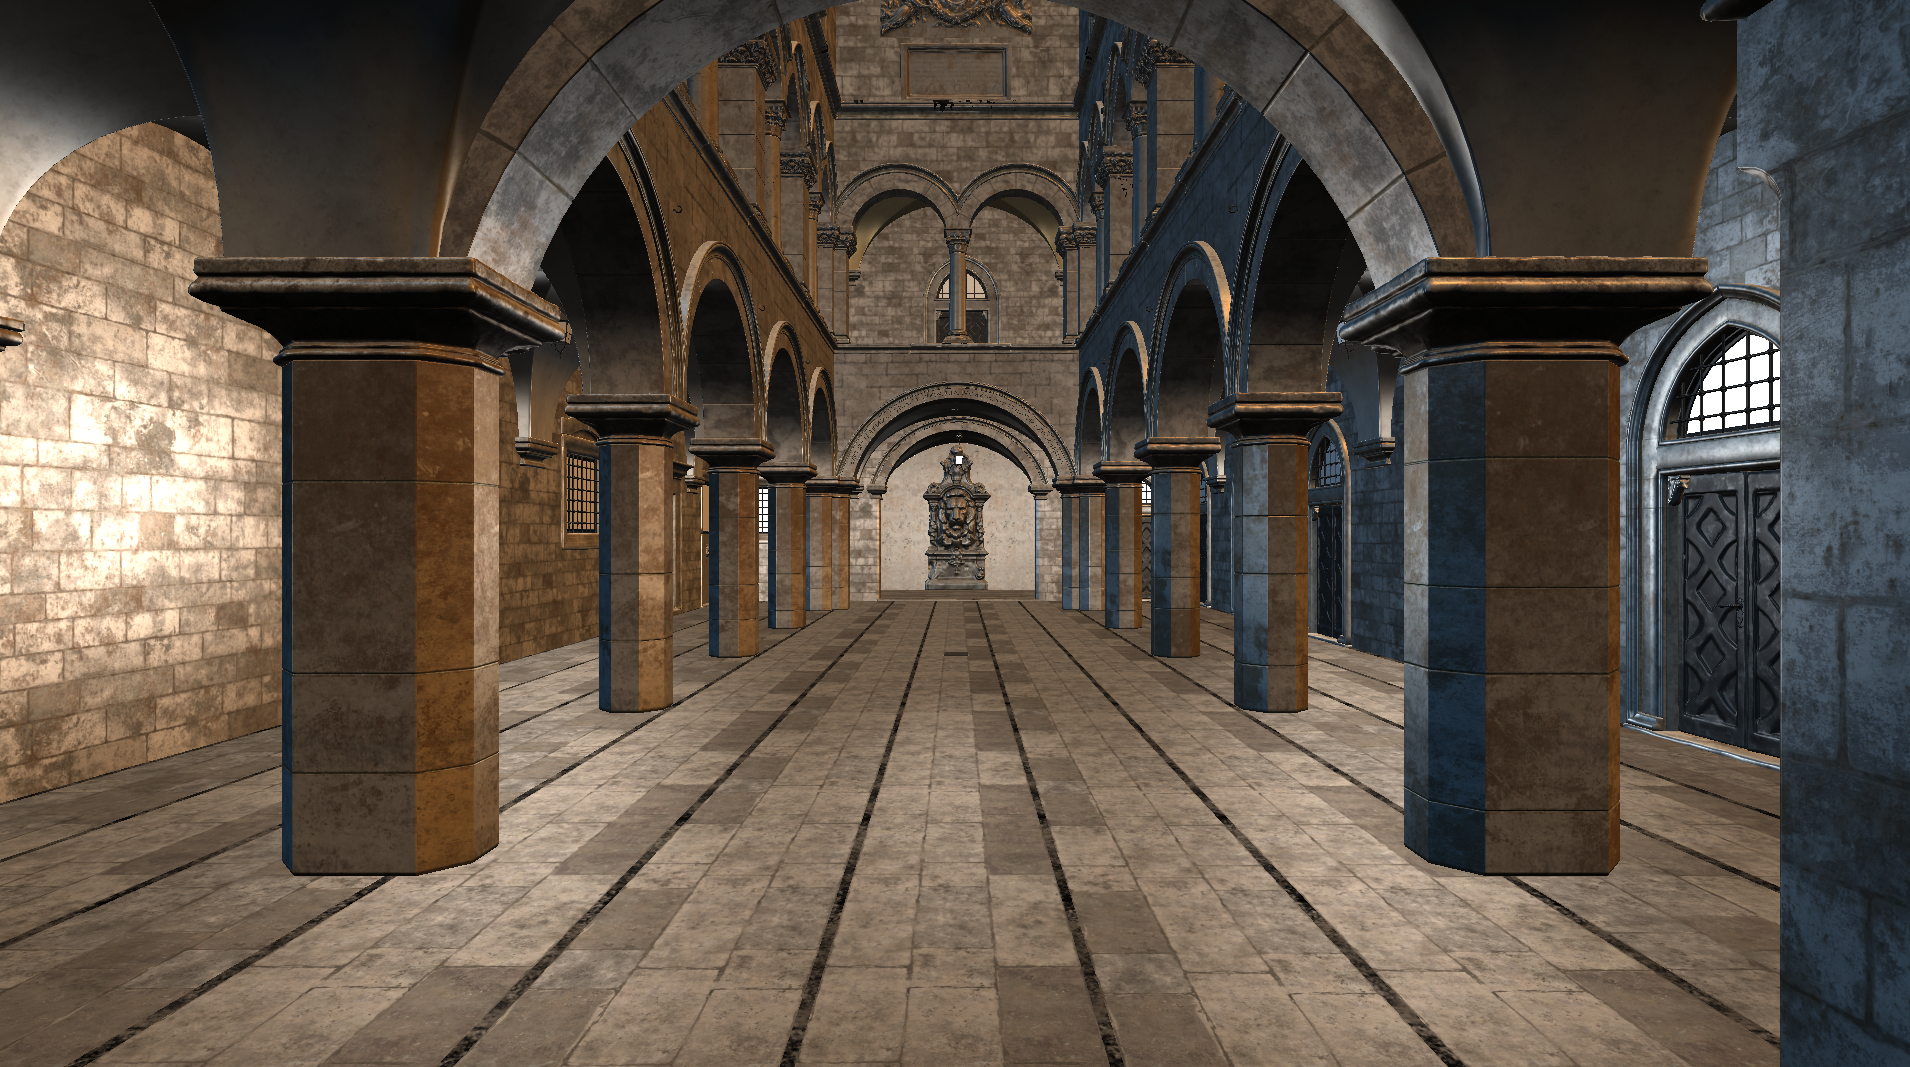
\includegraphics[width=\textwidth]{images/demo_sponza_1.png}
		\caption{Widok uproszczony.}
	\end{subfigure}
	\begin{subfigure}{.5\textwidth}
		\centering
		\includegraphics[width=\textwidth]{images/demo_sponza_1_pbr.png}
		\caption{Tryb PBR.}
	\end{subfigure}
	\caption{Hala atrium Sponza wygenerowana przez moduł.}
	\label{test_sponza_1}
\end{figure}

\begin{figure}[h!]
	\begin{subfigure}{.5\textwidth}
		\centering
		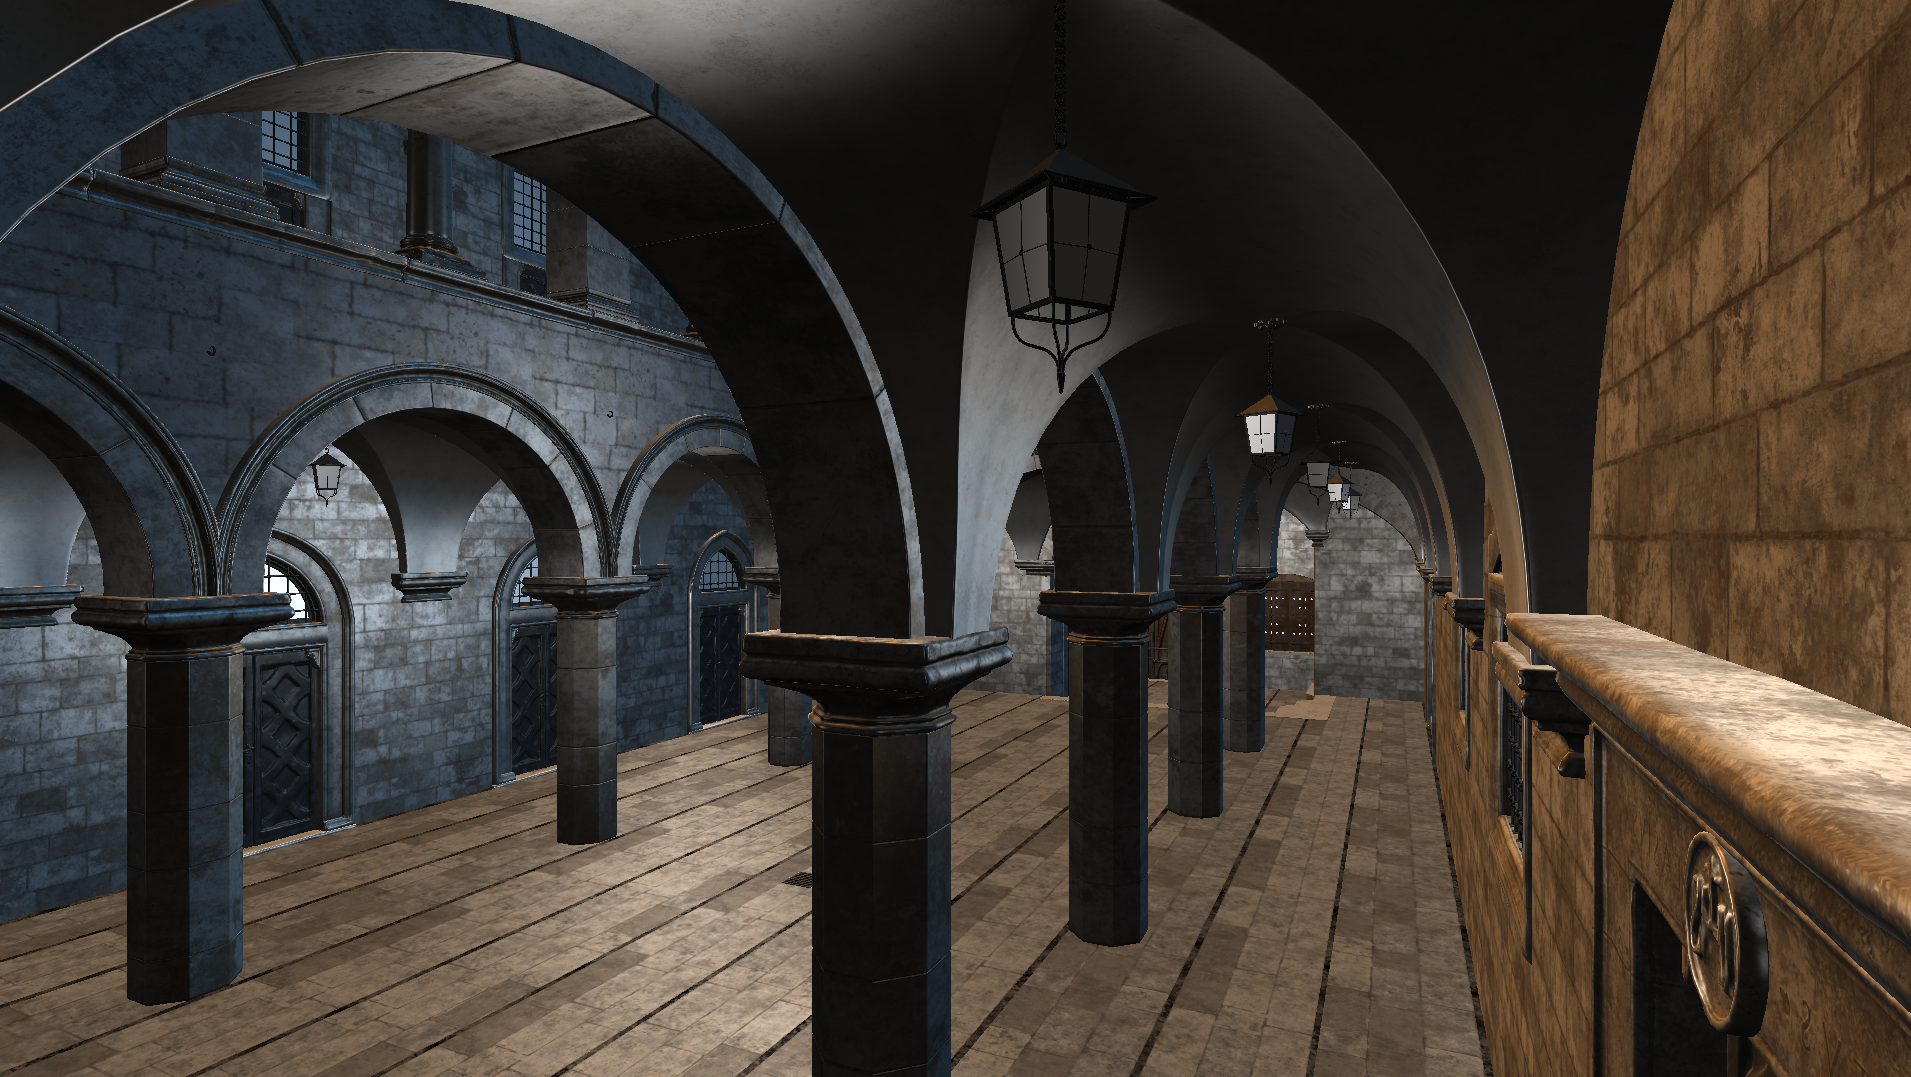
\includegraphics[width=\textwidth]{images/demo_sponza_2.png}
		\caption{Tryb klasyczny.}
	\end{subfigure}
	\begin{subfigure}{.5\textwidth}
		\centering
		\includegraphics[width=\textwidth]{images/demo_sponza_2_pbr.png}
		\caption{Widok PBR.}
	\end{subfigure}
	\caption{Zakrzywione stropy w korytarzach Sponza.}
	\label{test_sponza_2}
\end{figure}

\begin{figure}[h!]
	\begin{subfigure}{.5\textwidth}
		\centering
		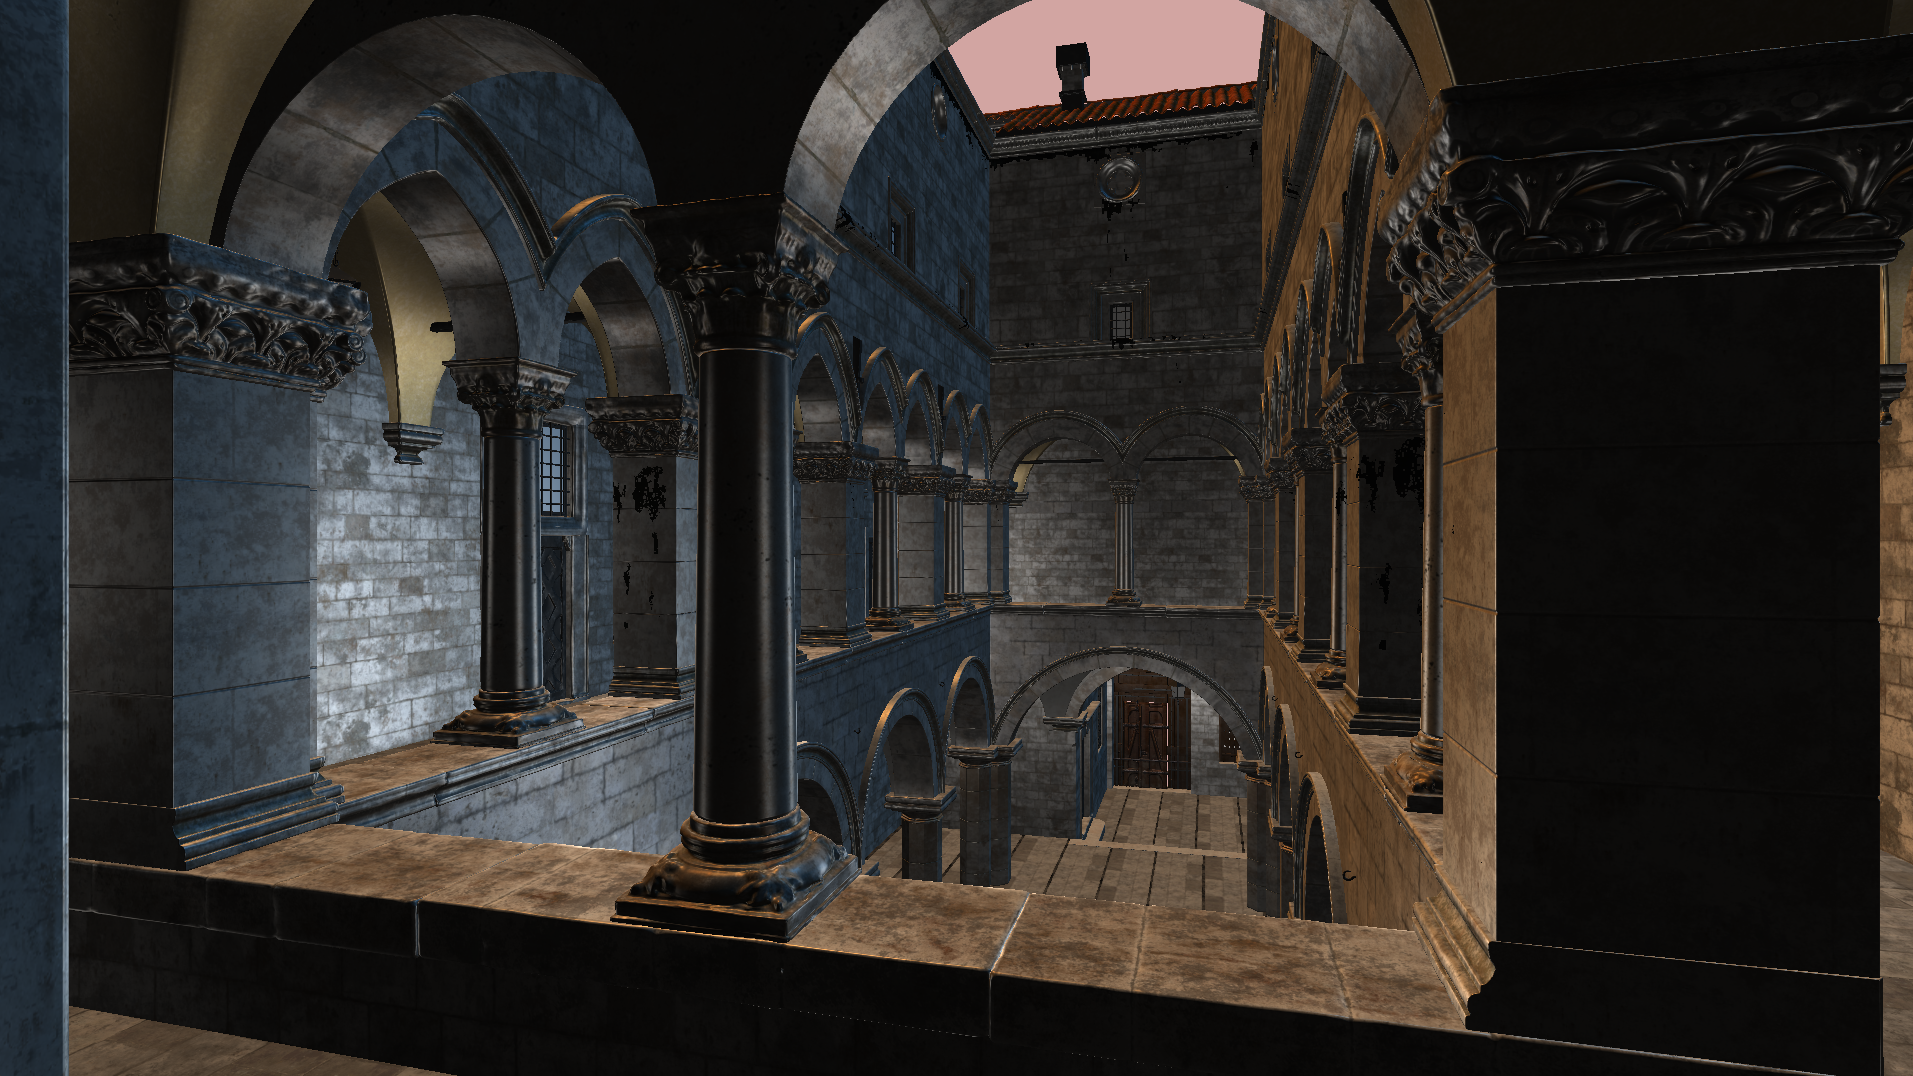
\includegraphics[width=\textwidth]{images/demo_sponza_4.png}
		\caption{Shader uproszczony.}
	\end{subfigure}
	\begin{subfigure}{.5\textwidth}
		\centering
		\includegraphics[width=\textwidth]{images/demo_sponza_4_pbr.png}
		\caption{Wersja oparta o Physically Based Rendering.}
	\end{subfigure}
	\caption{Widok z piętra pałacu.}
	\label{test_sponza_3}
\end{figure}

\vfill
\clearpage

\section{Demo detali - Roman Marble Plinth}
Opisywany już w rozdziale testów model \textit{Roman Marble Ornate Plinth} z pakietu Quixel Megascans został głównym obiektem tej sekcji, ze względu na dużą ilość detali geometrii i tekstur. Przedstawiony w dwóch wersjach na rys. \ref{test_highpoly} model charakteryzuje się wysokim narzutem wydajnościowym przy rysowaniu, co dało wyraźny znak przy określaniu wydajności dema, czego szczegóły zostały przedstawione w poniższej tabeli.

\begin{center}
	\begin{tabular}{ |l r r r|}
		\hline
		\textbf{Układ graficzny} & \textbf{FPS - uproszczony} & \textbf{FPS - PBR} & \textbf{Wydajność PBR} \\
		\hline
		NVIDIA 4060 & \textbf{360} & \textbf{445} & \textbf{123.61\%} \\
		Radeon 780M & \textbf{84} & \textbf{84} & \textbf{100.00\%} \\
		Procent wydajności & \textbf{23.33\%} & \textbf{18.88\%} & - \\
		\hline
	\end{tabular}
\end{center}

\begin{figure}[h!]
	\begin{subfigure}{.5\textwidth}
		\centering
		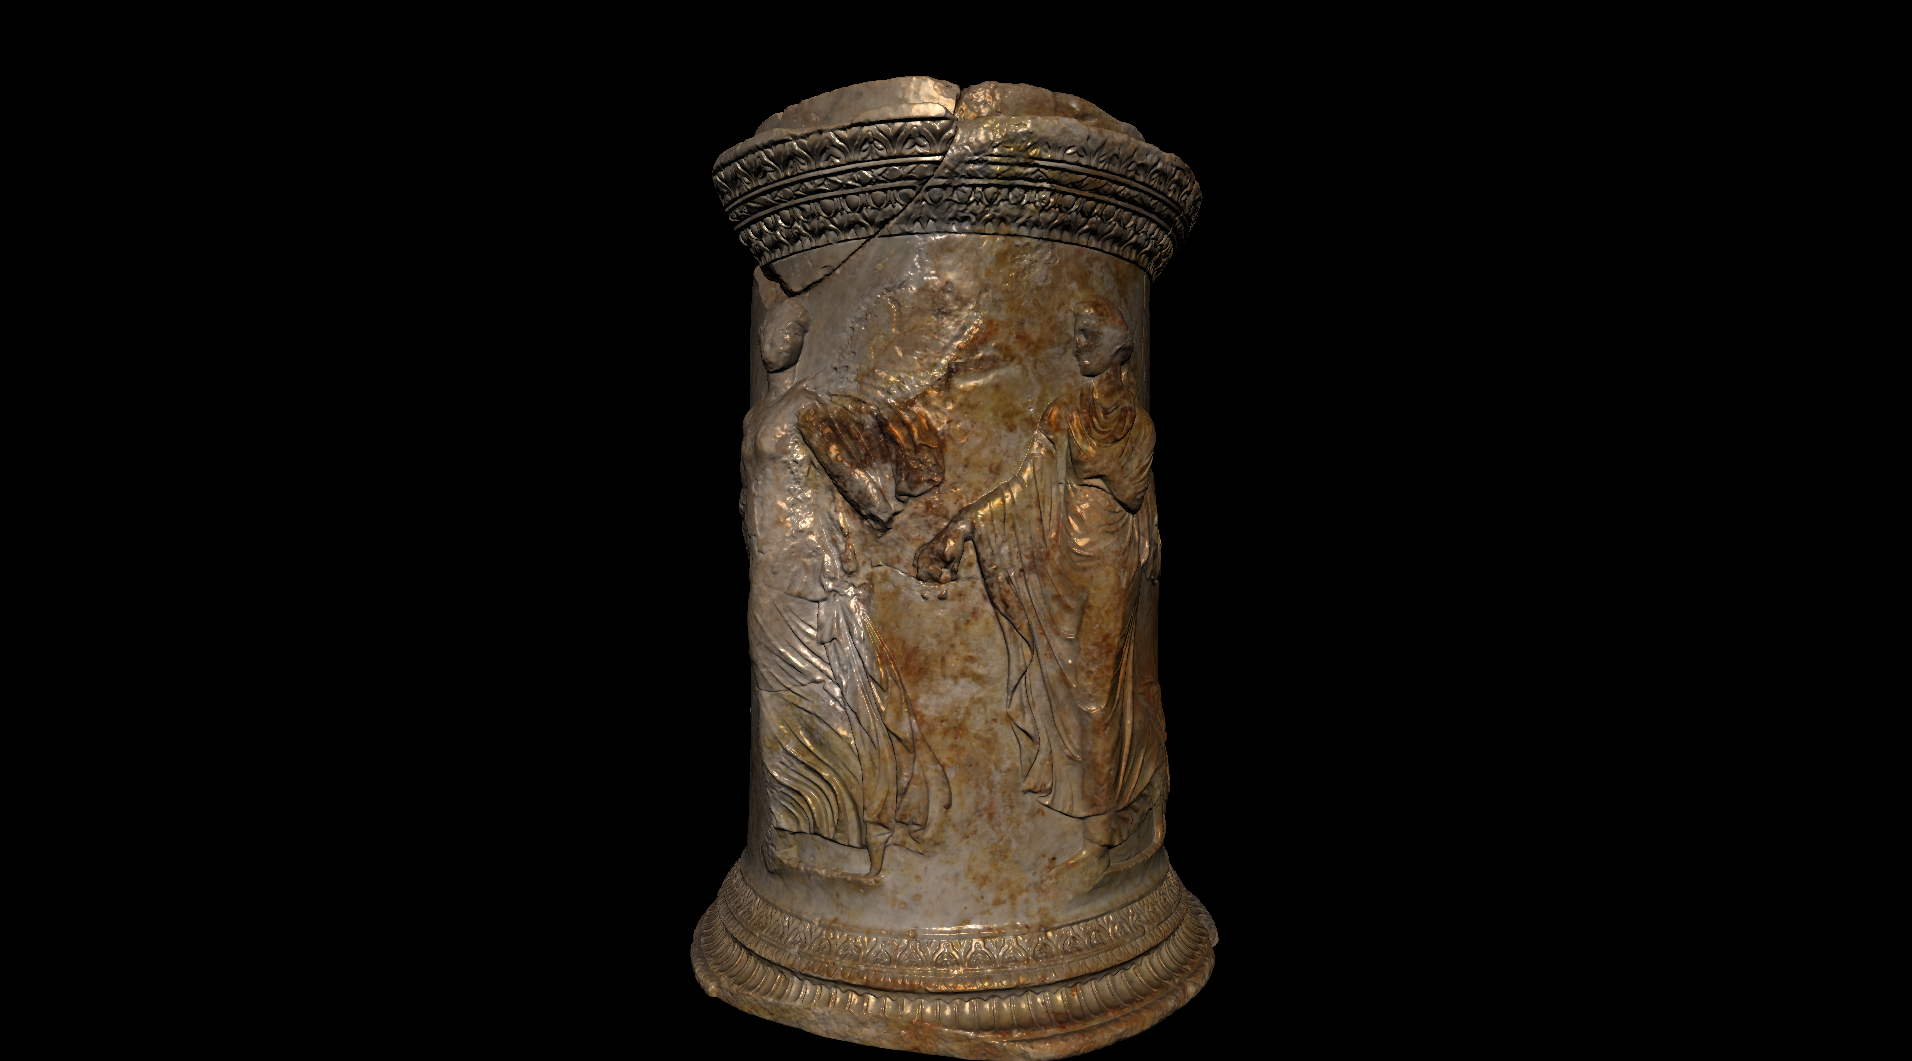
\includegraphics[width=\textwidth]{images/demo_highPoly.png}
		\caption{Wersja uproszczona.}
	\end{subfigure}
	\begin{subfigure}{.5\textwidth}
		\centering
		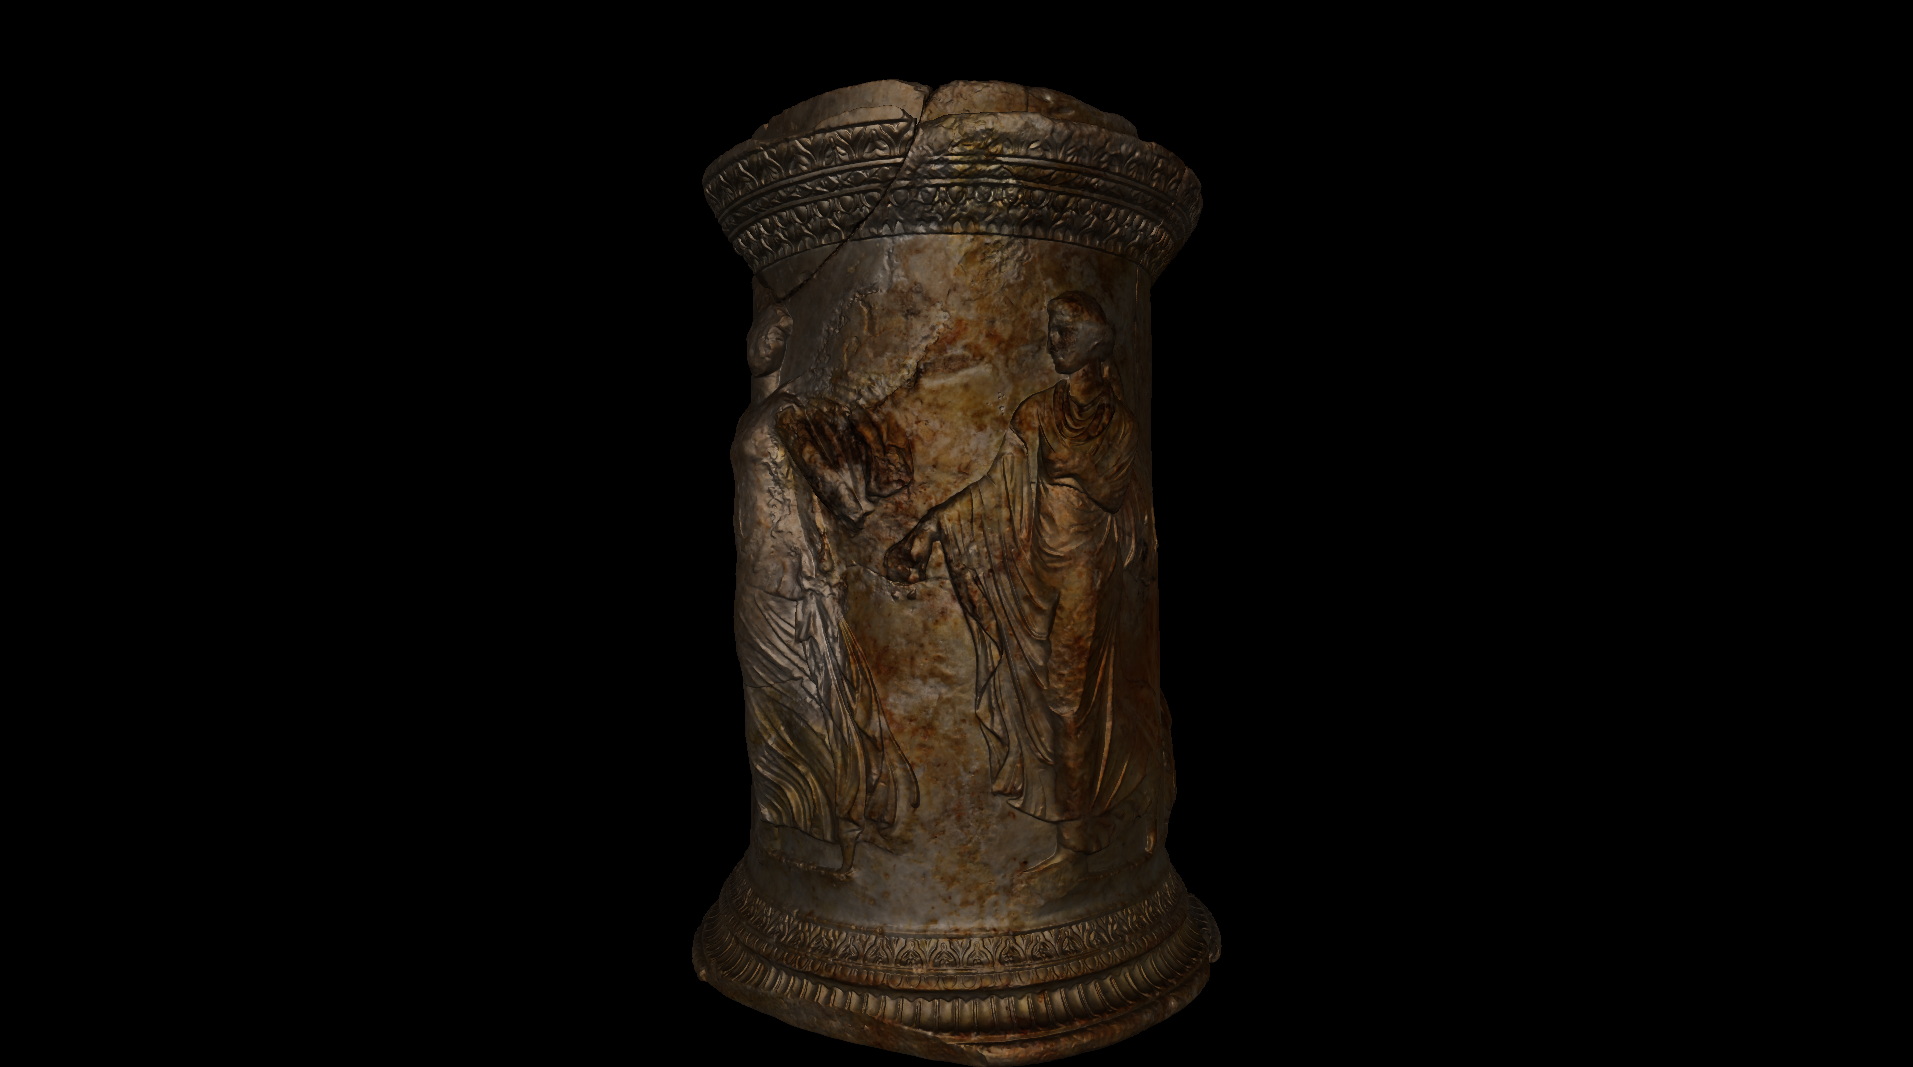
\includegraphics[width=\textwidth]{images/demo_highPoly_PBR.png}
		\caption{Tryb PBR.}
	\end{subfigure}
	\caption{Model cokołu w dwóch trybach działania modułu.}
	\label{test_highpoly}
\end{figure}

\section{Materiały}
Ostatnim demo przedstawiającym główne funkcjonalności modułu jest pokazanie możliwości zaimplementowanego systemu materiałów. Scena testu, pokazana na rys. \ref{demo_materials} składa się z 3 głównych części.
 
Głównym, środkowym elementem jest zbiór modeli kul o różnych parametrach materiałów. Elementy czerwone mają przypisany materiał typu PBR, a ich umieszczenie pokazuje różnice między jego parametrami. W osi pionowej od góry do dołu rośnie wartość chropowatości powierzchni - \textit{roughness}, a w poziomej od lewej do prawej parametr metaliczności. Kule zielone rysowane są przy pomocy uproszczonego materiału, a kolejne instancje zwiększają konfigurację chropowatości od lewej do prawej. 

Pozostałe segmenty przyjmują postać wydłużonych w pionie sześcianów, pokazujących bezproblemową możliwość doimplementowania dodatkowych materiałów. Wykorzystują one nowy materiał i przypisany do niego shader, niebędący częścią oryginalnego modułu, zwracający kolor odpowiadający pozycji na ekranie. Jego dwie instancje różnią się włączeniem i wyłączeniem kalkulacji oświetlenia, odpowiednio dla lewej i prawej wersji. 

Wygenerowana scena przedstawiona została na rys. \ref{demo_materials}.

\begin{figure}[h!]
	\centering
	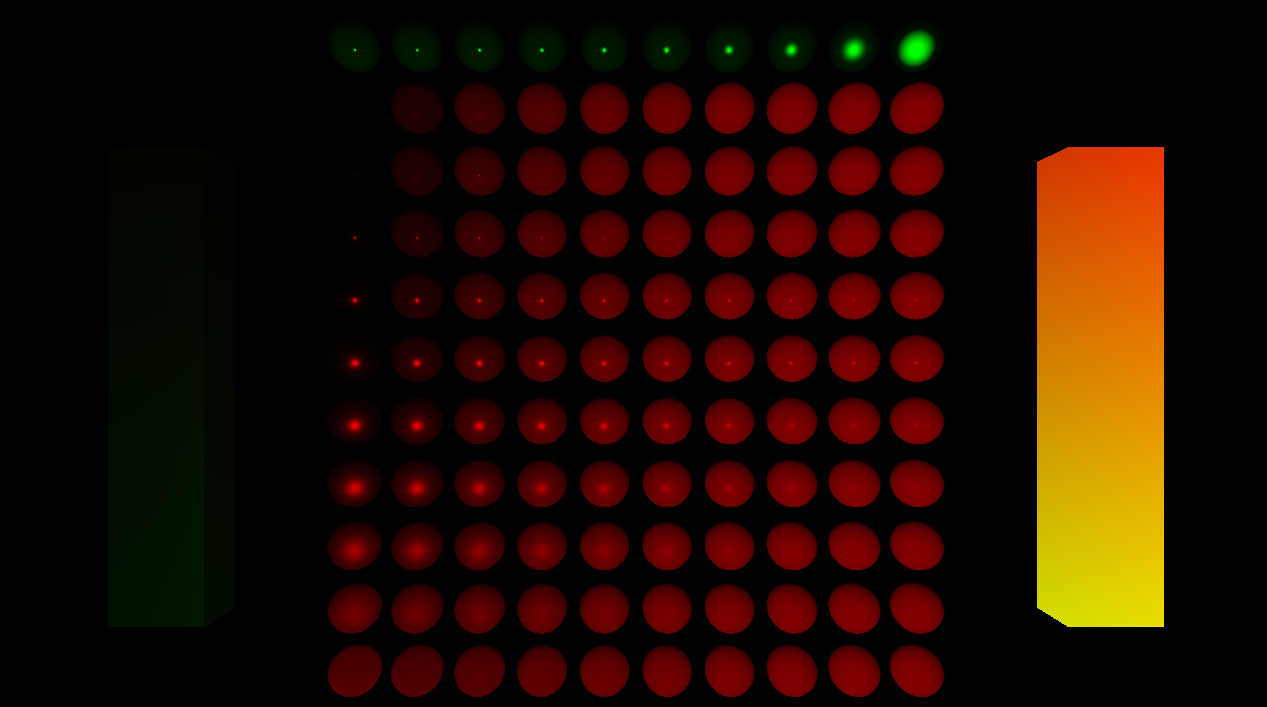
\includegraphics[width=\textwidth]{images/demo_materials.png}
	\caption{Zrzut ekranu przedstawiający obiekty o różnych materiałach i programach cieniujących.}
	\label{demo_materials}
\end{figure}

    % \include{rozdzial2}
    % \include{rozdzial3}



% itd.
% \appendix
% \include{dodatekA}
% \include{dodatekB}
% itd.

\printbibliography

\end{document}
